\documentclass[11pt,a4paper]{book}
\usepackage[english]{babel}
\usepackage{amsmath}
\usepackage{amsthm}
\usepackage{amsfonts}
\usepackage{amssymb}
\usepackage{graphicx}
\usepackage{geometry}
\usepackage[percent]{overpic}
\usepackage{tikz}
\usepackage[titletoc]{appendix}
\usepackage[round]{natbib}
\usepackage{glossaries}
\usepackage{longtable}
\usepackage{soul}

%\usepackage[usenames,dvipsnames,svgnames,table]{xcolor}
\definecolor{kuleuven}{RGB}{29,141,176}
\definecolor{kuleuven1}{RGB}{82,189,236}

\newcommand{\nocontentsline}[3]{}
\newcommand{\tocless}[2]{\bgroup\let\addcontentsline=\nocontentsline#1{#2}\egroup}

\newcommand\numberthis{\addtocounter{equation}{1}\tag{\theequation}}

\allowdisplaybreaks

\makeglossaries

\newglossaryentry{nps}
{
    name={Net Promotor Score (NPS)},
    description={Net promoter score is a widely used market research metric that typically takes the form of a single survey question asking respondents to rate the likelihood that they would recommend a company, product, or a service to a friend or colleague.}
}

\newacronym{ai}{AI}{Artificial Intelligence}
\newacronym{ml}{ML}{Machine Learning}
\newacronym{nlp}{NLP}{Natural Language Processing}
\newacronym{nlg}{NLG}{Natural Language Generation}
\newacronym{nlu}{NLU}{Natural Language Understanding}
\newacronym{hci}{HCI}{Human-Computer Interaction}
\newacronym{ahp}{AHP}{Analytical Hierarchy Process}
\newacronym{gdpr}{GDPR}{General Data Protection Regulation}
\newacronym{bipt}{BIPT}{Belgian Institute for Postal Services and Telecommunication}

\makeindex

\begin{document}
	%Start
	\frontmatter
\newgeometry{textwidth=540pt,textheight=780pt,top=20pt,left=20pt,right=20pt}
\begin{titlepage}
	
	\begin{figure}[t]{%
			\begin{overpic}[width=1\textwidth]{../LaTeX/Layout/Picture1.png}
				\put(46,4){\color{white}\large{\textbf{FACULTY OF ECONOMICS AND BUSINESS}}}
			\end{overpic}
		}
	\end{figure}
	
	\vspace*{4.5cm}
	{\color{kuleuven1}{\Huge  A study on the impact of customer service chatbots on the telecom industry}}
	
	\vspace*{0.5cm}
	{\Large The impact of a customer service chatbot on both business and customer side within the telecom industry.}
	
	\begin{figure}[b]
		%\centering
		\begin{minipage}[c]{0.4\textwidth}  {%
				\begin{overpic}[width=0.9\textwidth]{../LaTeX/Layout/Picture2.png}
					\put(70,45){\begin{minipage}[c]{1.80\textwidth}
							\begin{flushright}
								
								{\Large Rob De Putter, Mout Pessemier} \linebreak
								{r0836627, r0837708} \linebreak
								
								\textbf{{\large Thesis submitted to obtain \linebreak
										the degree of  master in Information Management}} \linebreak
								
								%!!!IMPORTANT!!!:
								%indicate the appropriate title of your master and major. Check the website https://feb.kuleuven.be/studentenportaal/contact/masterproef-leuven
								{\large Information Management}\linebreak
								\linebreak
								\textbf{{\large Promoter:}}   Prof.\ Dr.\ Jan Vanthienen \linebreak
								\textbf{{\large Supervisor:}} Vedavyas Etikala \linebreak
								
								%\linebreak
								
								\textbf{{\large Academic year:}} {\large 2021-2022}
								\linebreak
							\end{flushright}
					\end{minipage}}
				\end{overpic}
			}
		\end{minipage}
		
		
		\begin{picture}(540,0.2)
			\put(0,0){\colorbox{kuleuven1}{\makebox(540,0.2){}}}
		\end{picture}
	\end{figure}
	
\end{titlepage}
%%%%%%%%%%%%%%%%%%%%%%%%%%%%%%%%%%%%%%%%%%%%%%%%%%%%%%%%%%%%%%%%%%%%%%%%%%%%%%%%%%%%%%%%%%%%%%%%%%%% 

	\restoregeometry
\setcounter{equation}{1}

\pagestyle{empty}
\tableofcontents
	
	%Abstract & Thankword
	\chapter*{Abstract\hfill} \addcontentsline{toc}{chapter}{Abstract}
\label{ch:abstract}
\begin{flushright}
	Leuven, May, 2022.
\end{flushright}
%%%%%%%%%%%%%%%%%%%%%%%%%%%%%%%%%%%%%%%%%%%%%%%%%%%%%%%%%%%%%%%%%%%%%%%%%%%%%%%%%%%%%%%%%%%%%%%%%%%%%%%%%
\acrfull{ai} has grown ingrained in the \acrshort{it} sector, and technology is increasingly incorporated into our daily lives. Businesses are aware of this switch and are trying to use \acrshort{ai} to automate repetitive and ordinary work, which results in a more efficient and productive way of working. Customer service chatbots are an example of this. These "robots" are ideally capable of largely taking over the customer service from human agents. It is critical that these chatbots continue to produce high-quality work in order to improve customer experience and satisfaction, as this has a significant impact on customer trust and brand reputation.\\
\break
The goal of this research is to determine the impact of chatbots on companies' current and future strategies, as well as what customers expect from such a chatbot. The research is applied within the scope of the Belgian and Dutch telecom industries. Interviews with telecom companies such as Proximus, Telenet, T-Mobile, and KPN were done as part of this research, as well as a survey to get customer insights/expectations on these chatbots and what is important to them.\\
\break
The results show that in the future, telecom providers want to optimise their chatbots through data analysis, with sentiment analysis as the most common approach. From the importance study, it can be concluded that the chatbot should be easy to use and available 24/7.
	\chapter*{Thankword\hfill} \addcontentsline{toc}{chapter}{Thankword}
\label{ch:thankword}
First and foremost, we would like to thank our supervisor Vedavyas Etikala for guiding us through the entire process of this thesis. During difficult moments and hopeless situations he knew how to put us on the right track so that we could finish the thesis successfully. Besides our supervisor, we would also like to thank Prof. Dr. Vanthienen for his feedback and insights on the research. We would also like to thank Chatlayer for making their resources available to us so that we could experiment with chatbots in order to carry out the survey in a creative way, which was subsequently not elaborated on due to negative feedback. Furthermore, we would like to thank Sandrine d'Oreye, Nike Van Heeswijk, Laura Overwijk, Wisse Smet, Chiara Portolani and Justin Wesseling for taking part in the business interviews, through their enthusiasm and knowledge we were able to make interesting insights that have undoubtedly made a positive contribution to this research. We would also like to thank all 60 respondents for taking the time to fill in our survey carefully and qualitatively, without them there would be no research. A special thanks to Ella Raets for proof reading the thesis. To conclude, we would like to thank our parents, friends and fellow students who gave us moral support and motivation, and who made sure that studying was interspersed with entertainment.










	
	%Actual Text
	\mainmatter
\pagestyle{headings}

\chapter{Introduction}
Example citation: \cite{von2007theory}


\begin{figure}
	
\includegraphics[width=0.2\textwidth]{../LaTeX/Figures/Picture2.png}
	\caption{Example figure}
\end{figure}


	\mainmatter
\pagestyle{headings}

\chapter{Literature Study}
\label{ch:literature-study}

\section{What is a chatbot?}
A chatbot is a computer software program which combines \acrfull{nlp}, \acrfull{nlu} , \acrfull{nlg} \citep{Adamopoulou2020}, \acrfull{ai} and \acrfull{ml} algorithms to simulate a human-like behaviour. It can respond to questions and hold a conversation. This type of technology is what is called \acrfull{hci} \citep{Adamopoulou2020}.  \acrshort{hci} is most likely to become the most widely researched topic in the \acrshort{ai} community \citep{Bansal2018}. Chatbots are used in a variety of sectors such as education, health and of course e-commerce.\\
\break
The definition given by the dictionary goes as follows: “A computer program designed to simulate conversation with human users, especially over the Internet”\citep{Lexico2022}. Some more technical definitions are:
\begin{enumerate}
	\item A chatbot is an artificial intelligence program and a \acrfull{hci} model \citep{Bansal2018}.
	\item A chatbot is a software which act as tool that able to interact with human using human’s natural language with aim to assist human daily task \citep{Muizzah2021}.
	\item A chatbot  is  a  computer  program  which  responds  like  an  intelligent  entity when  conversed  with \citep{Khanna2015}.
\end{enumerate}\\
\break
Multiple types of chatbots exist, going from text-based to voice-based to a combination of both \citep{Radziwil2021}. Below is a more detailed taxonomy of chatbots.\\

\subsection{Taxonomy of a chatbot}
There are many variants of chatbots such as digital assistants, artificial conversation entities, interactive agents and smart bots \citep{Adamopoulou2020}. In this research, the focus will be on the interactive agents. Since these are made to support customer service, this research will mostly be focusing on interactive agents.\\
\break
These variants can be further divided into different categories. Chatbots can be categorise based on multiple factors such as:\\

\subsubsection{Architecture}
This categorisation is based on the way the chatbots are constructed, their internal architecture. Two types emerge: \textbf{rule-based} chatbots and \textbf{ai-based}. Rule-based chatbots use already developed or newly handcrafted algorithms as a decision maker to identify both knowledge and response. This model is fixed and can’t handle new inputs. On the other hand, \acrshort{ai}-based chatbots are chatbots that use \acrlong{ml} algorithms to generate a response based on the data provided. They keep on learning and improving based on the previous learning models. This way they are better equipped to handle new inputs \citep{Maroengsit2019}.\\

\subsubsection{Domain}
The domain category is based on how broad the domain is in which they are used. \textbf{Domain specific} chatbots focus on \textbf{specific industries}. They have knowledge of the industry they are deployed in. On the other hand, \textbf{general domain} chatbots are created to support conversations in \textbf{open topics}. They don’t support a specific domain. Instead, they are versatile and may be applied to any discipline \citep{Maroengsit2019}.\\

\subsubsection{Platform}
Chatbots can be divided up based on the platform on which they are active. \textbf{Social media} chatbots use platforms such as Facebook Messenger, Facebook WhatsApp or Telegram Messenger for their communication with the user. \textbf{Web based} chatbots are most common on websites of companies. There, they get their own chat box to serve clients that way. \textbf{Standalone program} chatbots are installed as a separate program on the device of the user \citep*{Maroengsit2019, Xu2017, CICBA2018}.\\

\subsubsection{Type of service provided}
\textbf{Goal-based} chatbots have a \textbf{set goal} they want to reach. For example, a set goal could be to sell a specific product to the customer. Once the product is sold, the chatbot has successfully reached its goal and thus fulfilled its purpose. \textbf{Knowledge-based} chatbots are classified on \textbf{the knowledge they possess}. \textbf{Service-based} chatbots are divided on \textbf{the services they provide} to the customer. Response-generated based chatbots are classified based on what action it performs in response generation \citep{Nuruzzaman2018}. It is possible that e.g., a goal-based chatbot can be a service-based or knowledge-based chatbot and vice versa.\\

\subsubsection{Task}
This categorisation results in \textbf{task-oriented} and \textbf{non-task-oriented} chatbots. The latter is more \textbf{question oriented} and the first one is \textbf{more conversational} \citep{Nuruzzaman2018}. Task-oriented chatbots aim to assist the customer to complete a certain task and have a short conversation. Examples are Siri, Google Now and Alexa. Non-task-orientd chatbots focus on conversing with the customers to answer questions and for entertainment purposes. \citep{Nuruzzaman2018}\\

\subsection{Some examples of e-commerce chatbots}
\begin{enumerate}
	\item Billie by Bol.com
	\item Stylebot by Nike
	\item The Proximus in-app chatbot
	\item Domino's AnyWare by Domino's Pizza
	\item Zalando chatbot
\end{enumerate}

\section{Customer service chatbots in the telecom industry: a deeper insight}
The telecom sector is an industry where customer satisfaction is an important factor. The different companies within this sector provide the same kind of services and products which makes switching operators easy. According to the research by \citep{Quintino2019}, the use of chatbots has a significant effect on customer satisfaction by ensuring better customer service. The findings from the research of \citeauthor{Quintino1019} were applied to Portuguese telecom companies, with this paper the line is further drawn into the Belgian telecom sector.\\
\subsection{The Belgian telecom industry: market overview}
The Belgian telecom sector is known as one of the most expensive in Europe, in the Eurostat survey conducted in 2019 it is even known as the most expensive in Europe \citep{Eurostat2020}. The services offered by the telecom operators can be divided into 2 categories: fixed internet and mobile.\\
\break
According to the 2020 annual report published by the \acrfull{bipt}, Proximus is the market leader in both fixed internet (45.3\%) and mobile (39\%). Telenet is in second place in both categories; for fixed Internet they have a market share of 35.6\%, for mobile this is 26\%. There is also a 3rd player that has been growing in recent years, Orange has a market share of 7.2\% in the fixed internet and +/- 26\% in the mobile market. \citep*{BIPT2021,VanLeemputten2021}.\\

\subsection{Challenges in the telecom industry}
Telecom operators in general face several challenges that can cause such companies to go bust. According to research by \citeauthor{Quintino2019} \citep*{Quintino2019, Malviya2012}, the most important challenges in this sector are: determining the revenue stream, rapidly changing consumer demands. The various challenges have an overall effect on customer retention. The findings from Quintino's research are also confirmed in Joshi's research \citep{Joshi2014}, in this paper, the parameters that affect the customer experience of cellular mobile services within the telecom industry of India are investigated \citep*{Joshi2014, Quintino2019, Malviya2012}.\\
\break
As in Quintino's study, this study will look at how the customer experience can be further optimised. It will be investigated how the chatbot can respond to the different challenges within the telecom sector. The results from this study can be used by telecom providers to further adjust their services to the needs of their (potential) customers.

\section{Key Attributes and components of a successful customer service chatbot}
Previous research \citep*{Muizzah2021, Verkeyn2018} has pointed out which characteristics are the most important. These characteristics can be grouped into some key dimensions provided by this previous research.\\

\subsubsection{Functionality}
The most important attributes are the interpretation of requests, execution of the request, flexible interpretation, ability to maintain a discussion, activation and the number of services available \citep*{Muizzah2021, Verkeyn2018}.\\

\subsubsection{Trustworthiness}
Trustworthiness handles about the chatbot containing dependable information, containing a wide range of knowledge, the possibility of rating the chatbot, robustness to unexpected input and transparency \citep*{Muizzah2021, Verkeyn2018}.

\subsubsection{Safety / Intrusion}
This category is all about protection and the respect of privacy and making sure the user is safe from intrusion \citep*{Muizzah2021, Verkeyn2018}.\\

\subsubsection{Efficiency}
The efficiency dimension specifies the ease of use, quick replies versus free text usage, availability, accessibility and the need for an account \citep*{Muizzah2021, Verkeyn2018}.\\

\subsubsection{Graphical Appearance}
Graphical Appearance is all about the design and feel of the user interface and the use of emojis and GIFs in conversations \citep*{Muizzah2021, Verkeyn2018}.\\

\subsubsection{Humanity}
The humanity dimension shows how human-like the chatbot is. The attributes are about how real the chatbot feels, if it creates and an enjoyable interaction, if it can convey a personality and if it can read and respond to certain moods of the customer \citep*{Muizzah2021, Verkeyn2018}.\\

\subsubsection{Empathy}
Empathy is about personalised options and suggestions \citep*{Muizzah2021, Verkeyn2018}.\\

\subsubsection{Responsiveness}
Responsiveness specifies the productivity and how fast the chatbot responds \citep*{Muizzah2021, Verkeyn2018}.\\
\break
By putting these 8 dimensions through \acrfull{ahp}, 7 main \acrshort{ahp} categories are found. \acrshort{ahp} is a structured approach for navigating complex decision-making processes that involve both qualitative and quantitative considerations \citep{Radziwil2021}. Table 1 lists the plausible attributes that give the highest user satisfaction score \citep{Muizzah2021}.\\

\begin{longtable}{|l|l|}
	\hline
	\textbf{Categories} &
	\textbf{Attributes} \\ \hline
	\endfirsthead
	\endhead
	\begin{tabular}[c]{@{}l@{}}Technical\\ Functionalities\end{tabular} &
	\begin{tabular}[c]{@{}l@{}}- Sentiment analytics: Intelligent (Using \acrshort{ai}, \acrshort{nlp}, \acrshort{ml}, \\ Semantic technology\\ - User friendly\\ - Automated\\ - Simple interface\\ - Interactive (using video, audio) to cater needs from different groups\\ - Multi-lingual\\ - General ease of use\end{tabular} \\ \hline
	Efficiency &
	\begin{tabular}[c]{@{}l@{}}- Robust to manipulation of data input by user\\ - Provide proper escalation channels\\ - Quick to answer\\ - Can perform damage control easily\end{tabular} \\ \hline
	Effectiveness &
	\begin{tabular}[c]{@{}l@{}}- Interpret statements and instructions accurately\\ - Linguistic accuracy\\ - Execute desired tasks correctly\\ - Contains wide array of knowledge\\ - Able to perform simple problem solving\end{tabular} \\ \hline
	Humanistic &
	\begin{tabular}[c]{@{}l@{}}- Human-like personality\\ - Transparent and disclose the chatbot identity\\ - Able to respond correctly to user's questions\\ - Can maintain the pattern of conversation within theme\end{tabular} \\ \hline
	Ethics &
	\begin{tabular}[c]{@{}l@{}}- Trained with knowledge of culture and ethics of users\\ - Protect and respect user's privacy\\ - Sensitive to user's concern (i.e., security, social concerns)\\ - Constancy\end{tabular} \\ \hline
	Technical Satisfaction &
	\begin{tabular}[c]{@{}l@{}}- Able to convey greetings\\ - Entertaining, fun and users enjoy the conversation\\ - Able to respond to the user's mood\\ - Provide emotional information using tones and expressions\end{tabular} \\ \hline
	Accessibility &
	\begin{tabular}[c]{@{}l@{}}- Ability to detect the user's intent\\ - Meeting a vast range of needs (i.e., time of buffer,\\ text interface)\\ - Available 24/7\end{tabular} \\ \hline
	\caption{Plausible quality attributes of Chatbot \citep{Muizzah2021}.}
	\label{tab:ChatbotAttributes}
\end{longtable}

These attributes can be brought under six quality assessment categories provided by the ISO 9126-1 quality model\footnote{https://www.iso.org/standard/22749.html} as seen in \ref{tab:ChatbotAttributes}.  By doing so, the quality of any piece of software, including a chatbot, can be measured \citep{Muizzah2021}.\\
\break
Depending on the goal you want to reach, the focus on the most important characteristics will shift \citep{Radziwil2021}. Overall, accessibility and efficiency come out to be the most important dimensions of a chatbot \citep{Radziwil2021}. Both \citep{Muizzah2021} and \citep{Radziwil2021} confirm these results.\\

\begin{longtable}{|c|c|}
	\hline
	\multicolumn{1}{|l|}{\textbf{Characteristics}} & \multicolumn{1}{l|}{\textbf{Sub Characteristics}}                                                            \\ \hline
	\endfirsthead
	\endhead
	Functionality   & \begin{tabular}[c]{@{}c@{}}Suitability\\ Accuracy\\ Interoperability\\ Security\\ Functional compliance\end{tabular}           \\ \hline
	Reliability                                    & \begin{tabular}[c]{@{}c@{}}Maturity\\ Fault tolerance\\ Recoverability\\ Reliability compliance\end{tabular} \\ \hline
	Usability       & \begin{tabular}[c]{@{}c@{}}Understandability\\ Learnability\\ Operability\\ Attractiveness\\ Usability compliance\end{tabular} \\ \hline
	Efficiency                                     & \begin{tabular}[c]{@{}c@{}}Time behaviour\\ Resource utilisation\\ Efficiency compliance\end{tabular}        \\ \hline
	Maintainability & \begin{tabular}[c]{@{}c@{}}Analysability\\ Changeability\\ Stability\\ Testability\\ Maintainability compliance\end{tabular}   \\ \hline
	Portability     & \begin{tabular}[c]{@{}c@{}}Adaptability\\ Installability\\ Co-existence\\ Replaceability\\ Portability compliance\end{tabular} \\ \hline
	\caption{the ISO/IEC 9126-1 internal/external quality model \citep{ISO9126}.}
	\label{tab:ISO9126}
\end{longtable}

\section{User experiences with customer service chatbots}
\subsection{How to interpret user experiences?}
In the past, customers could only make complaints and queries through mail or through a form. From 2016, this changed with the rise of \acrshort{ai} and the transition from online social networks to mobile messaging applications such as Messenger, WhatsApp, etc. Service providers tried to respond to this change by introducing chatbots for customer service \citep{Brandtzaeg2018}.\\
\break
Customer service chatbots offer the possibility to provide support to customers in real-time and around the clock. First of all, the chatbot will interpret the problem/question of the customer. Next, it will search in its model in which way it can best help the customer. Subsequently, the chatbot will execute the chosen approach until the customer's goal is reached.\\
\break
A chatbot for customer service must be tailor-made for the consumer. In the research performed by Brandtzaeg \& Følstad \citep{Brandtzaeg2018} it is mentioned that some companies push to introduce chatbots into their customer service, this then leads to a technological push. This push causes chatbots to become less qualitative and potentially lead to great frustrations for customers, therefore it is important that it contains the right features so that the consumer has a pleasant experience when coming into contact with the company. A pleasant experience in itself is difficult to measure, which is why this research will examine the various aspects of the user experience in this literature study.\\

\subsection{User’s perceptions of a chatbot}
\ul{Talking with a technology-based system}\\
According to the study "\acrshort{ai}-based chatbots in customer service and their effects on user compliance" \citep{Adam2021}, the interaction between the consumer/user and the system is fundamentally social. The consumer will still consider the chatbot as a social actor, even though it is already known that it cannot show emotions \citep{Adam2021}. In this research it can thus be considered that the consumer will interact with a chatbot in the same way as a human \citep*{Cheng2021,Ischen2020}.\\
\break
The study "Humanizing chatbots: The effects of visual, identity and conversational cues on humanness perceptions" proves otherwise. If an agent is known in advance as a chatbot, the user will biasedly evaluate whether the chatbot is of sufficient quality to meet their general expectations of machines. If the agent is marked as human, the user will evaluate the quality of the agent based on previous human interactions \citep*{Go2019,Shyam2008}.\\
\break
\ul{Efficiency and effectiveness}\\
The efficiency and effectiveness in performing a productive task is considered an important and crucial factor by consumers who are using a chatbot. The purpose of the chatbot is to make the user's life easier and more productive \citep{Brandtzaeg2018}.\\
\break
The study by \citeauthor{Skjuve2019} cites that the efficiency of the chatbot was one of the main motivators for the customers to use the chatbot, confirming once again that this quality attribute is crucial.\citep{Skjuve2019}\\
\break
\ul{Empathy}\\
The study “Exploring consumers' response to text-based chatbots in e-commerce: the moderating role of task complexity and chatbot disclosure” \citep{Cheng2021} concludes that empathetic factor of the chatbot is important for successful interactions. The empathetic factor of a chatbot makes the user's perspective more appreciated, it also makes it more responsive to the specific needs of the consumer.\\
\break
The study of \citeauthor{Agarwal2021} reaffirms that empathy has a positive influence on the interaction with the chatbot. Chatbots trained by data models that took more empathy/emotional into account responded in a similar way to human agents, in turn had a better impact on customer interaction. \citep{Agarwal2021}\\
\break
\ul{Task complexity}\\
The difficulty of a task given to the chatbot has a negative effect on consumer confidence. If the task is complex, the customer will have less confidence that the task will be completed successfully \citep{Cheng2021}.
This finding is confirmed by the research of \citeauthor{XU2020}, from the results of their experiment it was concluded that users expect humans to solve complex tasks better than an \acrshort{ai} device, such as a customer service chatbot. However, for tasks with low complexity, users expect that an \acrshort{ai} device could solve it better than humans. \citep{XU2020}\\
\break
\ul{Anthropomorphic visual cues}\\
Does a chatbot with visibly human characteristics affect user satisfaction? It is a question that plays a crucial role when researching the right user models. Anthropomorphic visual cues or visibly human features can provide a certain "humanity factor" \citep{Shyam2008}, which will make the consumer consider the chatbot more human and subsequently interact more socially \citep*{Go2019,Gong2007,Kim2012, Nowak2004}.
In addition \citeauthor{Go2019,Koda1996,Wexelblat1998} found that if a user interacts with an agent who has the same characteristics as him/herself (homogeneity), then the user will view the agent as positive. Studies have found that an agent with human characteristics is considered "better" than an agent with less human characteristics \citep*{Go2019,Koda1996,Wexelblat1998}.  
\\
\break
The study of \citeauthor{Go2019} shows that message interactivity contributes to compensating for low anthropomorphic visual cue, meaning that the interactivity of a chatbot is more important to users than the visual human characteristics \citep{Go2019}. Message interactivity in a conversation can be understood as the level of contingency in message exchange. In a conversation between two people, message interactivity means understanding another's message, as well as awareness of previous conversations, if these conditions are met, we can speak of an interactive and responsive conversation \citep*{Go2019,Sudweeks1998}.\\
\break
\citeauthor{Sheehan2020} stated that chatbots with more human characteristics are more readily adopted and can therefore be considered easier to use. \citep{Sheehan2020}
\section{What makes users trust a customer service chatbot?}
Customer trust is a crucial factor in customer service, and it is important that the customer accepts the agent's feedback as qualitative information. If the customer were to question the communication with the company, this could potentially lead to the loss of potential purchases. Measuring customer trust in a chatbot has already been investigated by \citeauthor{Folstad2018}. The research provides insight into different aspects of consumer trust within customer service.
\subsection{Interpretation of question}
The fact that the chatbot may not be able to interpret the questions correctly is a possible threat to the qualitative handling of a problem/question. If the questions are misinterpreted, it is possible that the chatbot shares wrong information. According to past research, consumers are more skeptical about the feedback from a chatbot when asked a complex question \citep*{Folstad2018,Nordheim2019}.\\

\subsection{Self-presentation}
A chatbot that reveals its weaknesses and limits are considered more trustworthy by consumers. The consumer gets a better idea of what may be asked and how confidential the information may be \citep{Folstad2018}.

\subsection{Security and privacy}
The consumer expects the chatbot to meet certain security levels, especially when the chatbot handles transactions that may contain personal data. The user assumes that the service provider is responsible when the chatbot fails to support transactions \citep*{Folstad2018, Nordheim2019}.\\
\break
Since the existence of \acrfull{gdpr}, users' views on giving up personal data to machines have changed, this transition is also noticeable in chatbots. Users of chatbots want to know what happens to their data and how it is stored, they expect as little personal data as possible to be stored \citep*{Folstad2018, Nordheim2019}. 

\section{Issues and errors in the current generation of customer service chatbots}
Even though the usage of chatbots can bring forth significant advantages, they are not free of drawbacks and threats. Below are highlighted some critical issues every company should take into account.

\subsection{Privacy and data security}
Many users who interact with a chatbot are scared that their data is being captured and (mis)used. Providers should take the right precautionary measures to ensure the safety of data and to inform for what the personal data will be used. Otherwise, the usage of a chatbot will be negatively impacted \citep*{Adamopoulou2020, Duka2021, Rese2020}.

\subsection{Shortcomings of customer expectations}
One of the biggest categories of mistakes are the shortcomings of customer expectations. This varies from failing to understand their request or intent, giving wrong answers, providing a poor quality of content as well as miscommunication errors. These issues leave a bad taste in the mouth of the customer and makes them not return to the company \citep*{Adamopoulou2020, Duka2021, Nichifor2021, Sheehan2020, Margot}.

\subsection{Bias}
Bias can be shown towards multiple facets such as race, gender and religion. When taking a closer look at gender, it is interesting to see that the bias comes from both directions. Chatbots can make biased remarks towards it's customers. At the same time study shows that the customer applies gender bias towards gender identified chatbots in the field of gender-stereotypical subject domains such as mechanics for male chatbots. It is important to reduce the bias as much as possible for a smoother interaction between both parties \citep*{Adamopoulou2020, McDonnell2019}. Gender neutral bots seem to receive high satisfaction ratings in comparison to male and female chatbots, even though they are generally perceived with more negative personality traits such as colder and less friendly \citep{McDonnell2019}.

\subsection{Toxic content and social harm}
Toxic content is a severe drawback for customers. Getting insulted and getting racial slurs thrown at your head is the last thing a customer wants when interacting with a chatbot. This issue is mostly present with chatbots that use each conversation as a learning ground. Malicious users such as internet trolls can fully impact and transform the vocabulary used by the chatbot in a matter of hours \citep{Adamopoulou2020}.\\
\break
Toxic content can be taken even a step further when applied to social network bots. An example might be a chatbot that tweets about racist things, claiming that someone has committed rape or abuse, murder etc. All of this is done with the intent to hurt someone or a group of people. This is all possible because these chatbots pass the Turing Test easily \citep{Radziwil2021}.

\subsection{Lack of knowledge about good and bad attribute types}
It is difficult to tailor a chatbot to the exact need of the customers. This is due to the fact that there isn't a clear understanding about what the user deems important or critical as a success factor. The absence of knowledge on this front makes for a poor chatbot user experience \citep{brandtzaeg2020}.

\subsection{Not understanding the capabilities of the chatbot}
When customers don't fully understand the capabilities of a chatbot, he can't optimally use the service provided. This may result in frustrations or unnecessary limitations due to the absence of knowledge. It is in a company's best intrest to clearly specify what capabilities their chatbot has \citep{brandtzaeg2020}.

	\mainmatter
\pagestyle{headings}

\chapter{Methodology}
\label{ch:methodology}
\section{Research Questions \& Hypotheses}
To determine the influence of chatbots on the telecom industry, various questions must be asked of the industry's participants. These inquiries are predicated on a hypothesis from which we begin our investigation.\\
\break
Even if reality suggests otherwise, the hypotheses are developed with a favourable expectation in mind.\\
\break
\textbf{Main Question: Do current customer service chatbots know what they are supposed to do?}\\
\break 
Five research questions were formulated to answer this main research question:

\subsubsection{RQ1: Are current customer service chatbots effective in helping people and solving their problems?}
It is illogical to think that there will be people who will keep a good impression of a customer service chatbot after it was unable to help with or solve their existing problem. Multiple studies suggest that it is essential that the execution done by a chatbot is effective \citep*{Muizzah2021, Brandtzaeg2018}.\
In a task- oriented chatbot, under which a customer service chatbot can be placed, usefulness is key \citep{brandtzaeg2020}. Solving problems and providing help in an effective and efficient manner is the key to providing a good user experience. It is also crucial that the user's intentions are correctly interpreted and answered adequately.\\
\break
\citep{Verkeyn2018} categorized 28 quality attributes and divided them up in 5 dimensions. Based on these quality attributes, the evaluation of a chatbot is possible (see literature study). Relevant quality attributes that can be linked to the research question serve as the foundation for the hypotheses. In this way, the research question can be reliably tested against reality.\\
\break
\break
Related hypotheses:
\begin{enumerate}
	\item H1: Current customer service chatbots execute requested tasks correctly. Based on \citep{Verkeyn2018} quality attribute “Execute requested tasks” from the dimension “Functionality”
	\item H2: Current customer service chatbots can deliver the same services as a human agent. Based on \citep{Verkeyn2018} quality attribute “Number of services available in the chatbot” from the dimension “Functionality” (reference: \citep{Eeuwen2017})
	\item H3: Current customer service chatbots contain enough knowledge to provide good assistance. Based on \citep{Verkeyn2018} quality attribute “Contains breadth of knowledge” from the dimension “Trustworthiness” (reference: \citep*{Cohen2016, Kuligowska2015})
\end{enumerate}

\subsubsection{RQ2: Are current customer service chatbots easy to use and accessible?}
When a customer service chatbot is effective in helping people, but is so complex or unusable that nobody uses it again, it is rational to assume that this chatbot has not made a good impression. In addition, a chatbot should be easily accessible, so that a high level of service is always present.\\
Here, too, the quality attributes of \citep{Verkeyn2018} serve as the basis for evaluation. Relevant quality attributes that can be linked to the research question serve as the foundation for the hypotheses. In this way, the research question can be reliably tested against reality.\\
\break
\break
Related hypotheses:
\begin{enumerate}
	\item H4: Current customer service chatbots are easy to use. Based on \citep{Verkeyn2018} quality attribute “Ease of use” from the dimension “Efficiency” (reference:\citep*{Candela2018, Duijst2017})
	\item H5: Current customer service chatbots are available at all times (24/7). Based on \citep{Verkeyn2018} quality attribute “Available at all times” from the dimension “Efficiency” (reference: \citep{Wang2019})
\end{enumerate}

\subsubsection{RQ3: Do current customer service chatbots create a pleasant customer experience?}
When a customer uses a service or buys a product from a company, it is important that the customer has a good feeling about how this interaction went. When using a chatbot, a company wants to invoke a good feeling in the user as well. \\
\break
A “pleasant” customer experience can be seen as an experience where the customer is helped in a friendly and smooth way.\\
\break
\break
Related hypotheses:
\begin{enumerate}
	\item H6: Current customer service chatbots create an enjoyable interaction Based on \citep{Verkeyn2018} quality attribute “Create an enjoyable interaction” from the dimension “Humanity” (reference: \citep{Morrissey2013})
\end{enumerate}

\section{Methodology - Business Interviews}
To gain more insight into what the customer service chatbot means for telecom businesses, an exploratory research was conducted through interviews. The interviews were conducted with conversational designers, product owners, developers and AI trainers from Proximus, Telenet, T-Mobile and KPN. Each interview was conducted online through Teams-meetings. The write-outs of these interviews can be found in the \ref{ch:appendices}ppendices\\
\break
The interview consists of four main parts:
\begin{enumerate}
	\item The current state of the customer service chatbot;
	\item The benefits that the company derives from the presence of the chatbot;
	\item The business value (revenue, reduced costs) realised by the chatbot;
	\item The company's future vision of the chatbot.
\end{enumerate}

\subsection{The current state of the customer service chatbot}
The chatbot's general specifications were questioned in the first phase. This can be explained in terms of the chatbot's capabilities (FAQs, complaint handling, sales, etc. ), the platforms on which the bot can be found, the languages in which the bot can be addressed, the age group of the relevant users, and the types of questions the bot can answer (yes/no questions, open/vague questions).\\

\subsection{The benefits that the company derives from the presence of the chatbot}
The second section focuses on the specific benefits that the firm receives from using the chatbot. For example, the chatbot is asked what services it can provide. This primarily pertains to renewing or forming a new membership, purchasing products/services, obtaining specific invoice details, and so on. The question also asks to what extent the chatbot can reduce customer support workload, and then goes into further depth about how many questions or tasks a chatbot cannot perform on its own. Furthermore, the focus is on how eager clients of the providers are to use a chatbot. Finally, the negative aspects of the story are discussed. One questions asks, for example, if there is more frustration among customers and whether customers trust the chatbot.\\

\subsection{The business value (revenue, reduced costs) realised by the chatbot}
The third part is about the business value that is created. First, it looks at how much extra direct turnover is created by the chatbot. Then it looks at how this value is generated, it asks about the availability of the chatbot, and how it handles conversations when no physical agents are present. Next, it looks at what the initial strategic goal of the chatbot was, was it just added to improve customer service, or was it more of a marketing stunt?  It also asks how much the chatbot costs and which cost items were the most expensive. Finally, it looks at how many fewer people are employed in customer service because of the chatbot.\\

\subsection{The company's future vision of the chatbot}
The fourth and final part focuses on the company's future vision of the chatbot. They look at the extra features they want to add and how they want to improve the chatbot in terms of technology. The latter could include sentiment analysis, fully AI driven, and so on. Finally, they are asked how they determine what scenarios/dialogs they want to put in the bot and how they will apply this in the future.\\

\section{Methodology - Survey}
The research questions and hypotheses will be investigated by means of a joint survey.\\
\break
These two strategies will be used to generate the most amount of business value possible. For the business, the value is created by comparing the competition and gathering insight into what the customers consider important. For the customer is the value found in better chatbots as a result of the study.\\

\subsection{Are these attributes present for the specific chatbot?}
To find out if the selected attributes are present, several questions will be used to check with the clients using the chatbots. The used questions per research question are listed below.

\subsubsection{RQ1: Are current customer service chatbots effective in helping people and solving their problems?}
\begin{itemize}
	\item H1: Current customer service chatbots execute requested tasks correctly.
	\begin{itemize}
		\item Did the chatbot fulfil your task correctly?
	\end{itemize}
	\item H2: Current customer service chatbots can deliver the same services as a human agent.
	\begin{itemize}
		\item Does the chatbot deliver the same services as a human?
	\end{itemize}
	\item H3: Current customer service chatbots contain enough knowledge to provide good assistance.
	\begin{itemize}
		\item Did the chatbot contain enough knowledge to help with your problem?
	\end{itemize}
\end{itemize}

\subsubsection{RQ2: Are current customer service chatbots easy to use and accessible?}
\begin{itemize}
	\item H4: Current customer service chatbots are easy to use.
	\begin{itemize}
		\item Was the chatbot easy to use?
	\end{itemize}
	\item H5: Current customer service chatbots are available at all times (24/7).
	\begin{itemize}
		\item Is the chatbot available at all times?
	\end{itemize}
\end{itemize}

\subsubsection{RQ3: Do current customer service chatbots create a pleasant customer experience?}
\begin{itemize}
	\item H6: Current customer service chatbots create an enjoyable interaction.
	\begin{itemize}
		\item Did you enjoy interacting with the chatbot?
	\end{itemize}
\end{itemize}
\ul{Rating scale}\\
For answering the statements, yes/no questions will be used to check the presence of these attributes.\\

\subsubsection{Data Evaluation Method - Comparative Study}
Both providers’ chatbots will be compared to one another to see which attributes are present in which chatbot.\\

\subsection{How important are these attributes for the clients?}
The research questions and hypotheses will be investigated/evaluated by means of the proven KANO method. The method of application is inspired by the study of \citep{Verkeyn2018}.\\
\break
To find out which of the chose 6 attributes types are seen as important, the following questions per category will be used.

\subsubsection{Under ``Effective in helping people and solving their problems"}
\begin{enumerate}
	\item Execute requested tasks
	\begin{itemize}
		\item The chatbot (DOES NOT) execute(s) every/any requested task that can reasonably be expected to be executed successfully.
	\end{itemize}
	\item Number of services available in the chatbot
	\begin{itemize}
		\item The chatbot can (NOT) perform the same services as a human agent.
	\end{itemize}
	\item Contains breadth of knowledge
	\begin{itemize}
		\item The chatbot knows at least as much as an expert in the same industry/service./ The chatbot knows less than an expert in the same industry/service.
	\end{itemize}
\end{enumerate}

\subsubsection{Under "Ease of use and accessibility"}
\begin{enumerate}
	\item Ease of use
	\begin{itemize}
		\item The chatbot is (NOT) self-explanatory in its use.
	\end{itemize}
	\item Available at all times
	\begin{itemize}
		\item The chatbot is (NOT) available at all times.
	\end{itemize}
\end{enumerate}

\subsubsection{Under "Pleasant customer experience"}
\begin{enumerate}
	\item Create an enjoyable interaction
	\begin{itemize}
		\item The chatbot (DOES NOT) communicate(s) in a robotic, non-empathic way./ The chatbot interacts in an enjoyable way.
	\end{itemize}
\end{enumerate}
\ul{Rating scale}\\
For answering the statements, a five-level rating scale in the spirit of the one drawn up by \citep{KANO1984}, will be used.\\
\break
The levels are as follows:\\
\begin{enumerate}
	\item I dislike it
	\item I can live with it
	\item I am neutral
	\item I expect it
	\item I like it
\end{enumerate}
This scale allows users to express how much they agree with a given statement.\\

\subsubsection{Data Evaluation Method - Comparative Study}
To be able to answer the second main question, there is a need for an evaluation method that will list the general user importance for each quality attribute. Kano is a tool that can satisfy these desires. The Kano Model gives more insight into the fact that the performance of the quality attributes is not in a linear relationship with the corresponding customer satisfaction \citep{KANO1984}. Kano offers the possibility to divide the quality attributes into five categories that each have different effects on customer satisfaction (Attractive, Performance, Must-Be, Indifferent, Reverse). This division is done on the basis of the answers obtained from the survey (questions with five-level rating scale).\\

\begin{figure}[ht]
	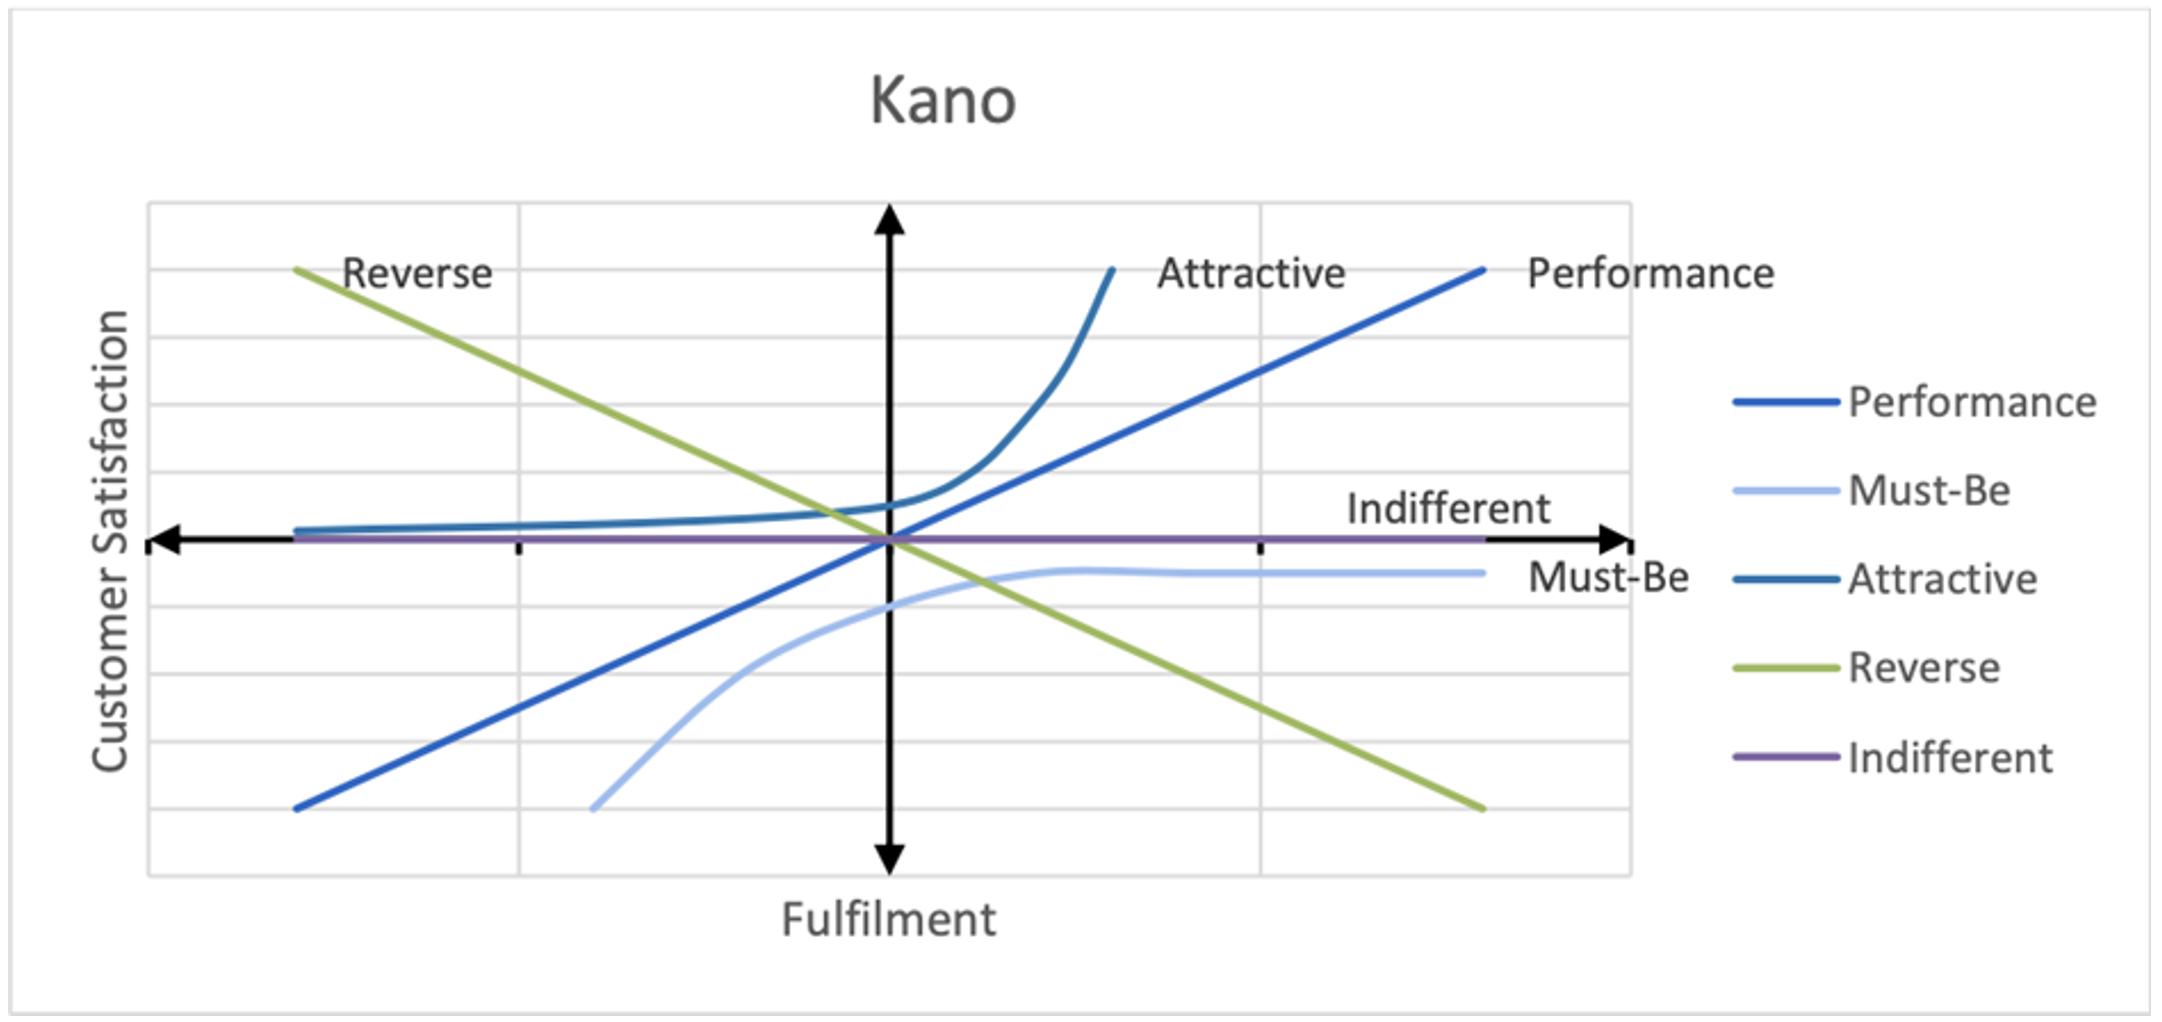
\includegraphics[scale=0.35]{../LaTeX/Figures/KANO.png}
	\caption{Five categories of quality attributes \citep{KANO1984}.}
	\label{fig:kano}
\end{figure}
\break
The five categories can be represented visually as in Figure \ref{fig:kano}, each category showing a different relationship.\\
\break
Attractive: if a quality attribute from this category is more present, the customer satisfaction will increase more than linearly. When the quality attribute is not present, the customer will have neither a positive nor negative customer satisfaction.\\
\break
Performance: When a quality attribute from this category is present, the customer satisfaction will increase linearly. If the quality attribute is not present, then this will result in a negative customer satisfaction.\\
\break
Indifferent: If a quality attribute from this category is present, then this has no effect on customer satisfaction.\\
\break
Must-Be: The customer considers this kind of quality attribute as necessary, when it is not present, the customer satisfaction will be drastically low and the product basically has failed at this point.\\
\break
Reverse: The more these quality attributes are present, the worse the customer satisfaction. The customer satisfaction increases when they are less present.\\

\subsection{Survey arrangement}
The survey is divided up into 3 parts:\\
\break
\ul{Part 1 - general information about the participant and information on the interaction with the chatbot}\\
\break
In the first part, general information about the participant is requested so that we can get a better idea of the person. The postal code, age, highest obtained degree, and gender are requested, these variables can be added as control variables in the static models to process the results.\\
\break
Next, they are asked from which company they used the chatbot, what task they performed, in what language they addressed the chatbot and on what platform they addressed the chatbot.\\
\break
\ul{Part 2 - questions about the interaction with the chatbot}\\
\break
The second part focuses on the interaction with the chatbot, the questions that were drawn up for the hypotheses in section \textbf{3.3.1 of the Methodology} are asked here. The results of this study are used to evaluate each company's chatbot, then a comparative study is conducted to determine which chatbot performs best.\\
\break
\ul{Part 3 - questions about the customer expectations of a telecom customer service chatbot}\\
\break
The third and final part of the survey asks what the customer expects from customer service chatbot in various scenarios. In order to put the participant in a certain context, three different scenarios were created in which a customer might find himself with the corresponding telecom services. The three scenarios are as follows:
\begin{enumerate}
	\item You haven't switched off your phone in a while and it suddenly ran out of battery. You have a problem because you don't remember your PIN code. You ask the chatbot if he can retrieve your PIN code given your client details. 
	\item You're not happy with your subscription because it doesn't match your needs, from a friend you've heard there is a better deal and so you want the chatbot to stop your subscription.
	\item At least once each month, you lose internet connectivity. You're sick and tired of these problems and you want to file a formal complaint. You turn to the chatbot of your telecom provider with your complaint.
\end{enumerate}
After a participant is introduced to each scenario, he/she is asked each time to give his/her opinion on the statements drawn up in \textbf{3.3.2 of the Methodology}. As already mentioned, the statements are questioned using a 5 rating scale, this terminology will then be used in the result processing through the KANO model.

\subsection{Target group}
The target group of our survey will not be filtered on age or other human characteristics, but it will be screened on whether the person has already had an experience with a telecom chatbot of a provider located in Belgium or in the Netherlands. The fact that the person already has experience with a telecom chatbot is crucial, otherwise the input for the comparative study is invalid.

	\mainmatter
\pagestyle{headings}
\chapter{Research}
\label{ch:research}

\section{Analysis}
The whole data set and data analysis script can be found on the GitHub repository\footnote{https://github.com/MoutPessemier/A-Survey-On-The-Impact-of-Customer-Chatbots-on-E-commerce}.\\
\break
The data has been anonymised in Excel. A new column was created called 'taskCategory'. The tasks performed are categorised in one of the following 4 categories:
\begin{itemize}
	\setlength\itemsep{-0.1em}
	\item FAQ
	\item Personalised question
	\item Complaint
	\item Sales
\end{itemize}
From the 65 entries, 5 had to be thrown away:
\begin{itemize}
	\setlength\itemsep{-0.1em}
	\item 3 because of the used chatbot: they were not telecom chatbots.
	\item 1 entry was a duplicate.
	\item 1 entry responded with one answer only (only yes and only neutral in part 2)
\end{itemize}

\subsection{Environment Variables}
\subsubsection{Age}
The mean and standard deviation values for each provider respectively are:
\begin{itemize}
	\setlength\itemsep{-0.1em}
	\item \textbf{Overall: 26.28 \& 7.49}
	\item Telenet: 26.96 \& 9.73
	\item Proximus: 27.26 \& 6.07
	\item Orange: 22.5 \& 2.12
	\item T-Mobile: 22.44 \& 2.01
	\item KPN: 27.75 \& 3.59
\end{itemize}
Next to the plot, there is a frequency table that shows the different values for age appearing in this survey, ordered from most common to least common.

\begin{figure}[!htb]
	\minipage{0.75\textwidth}
	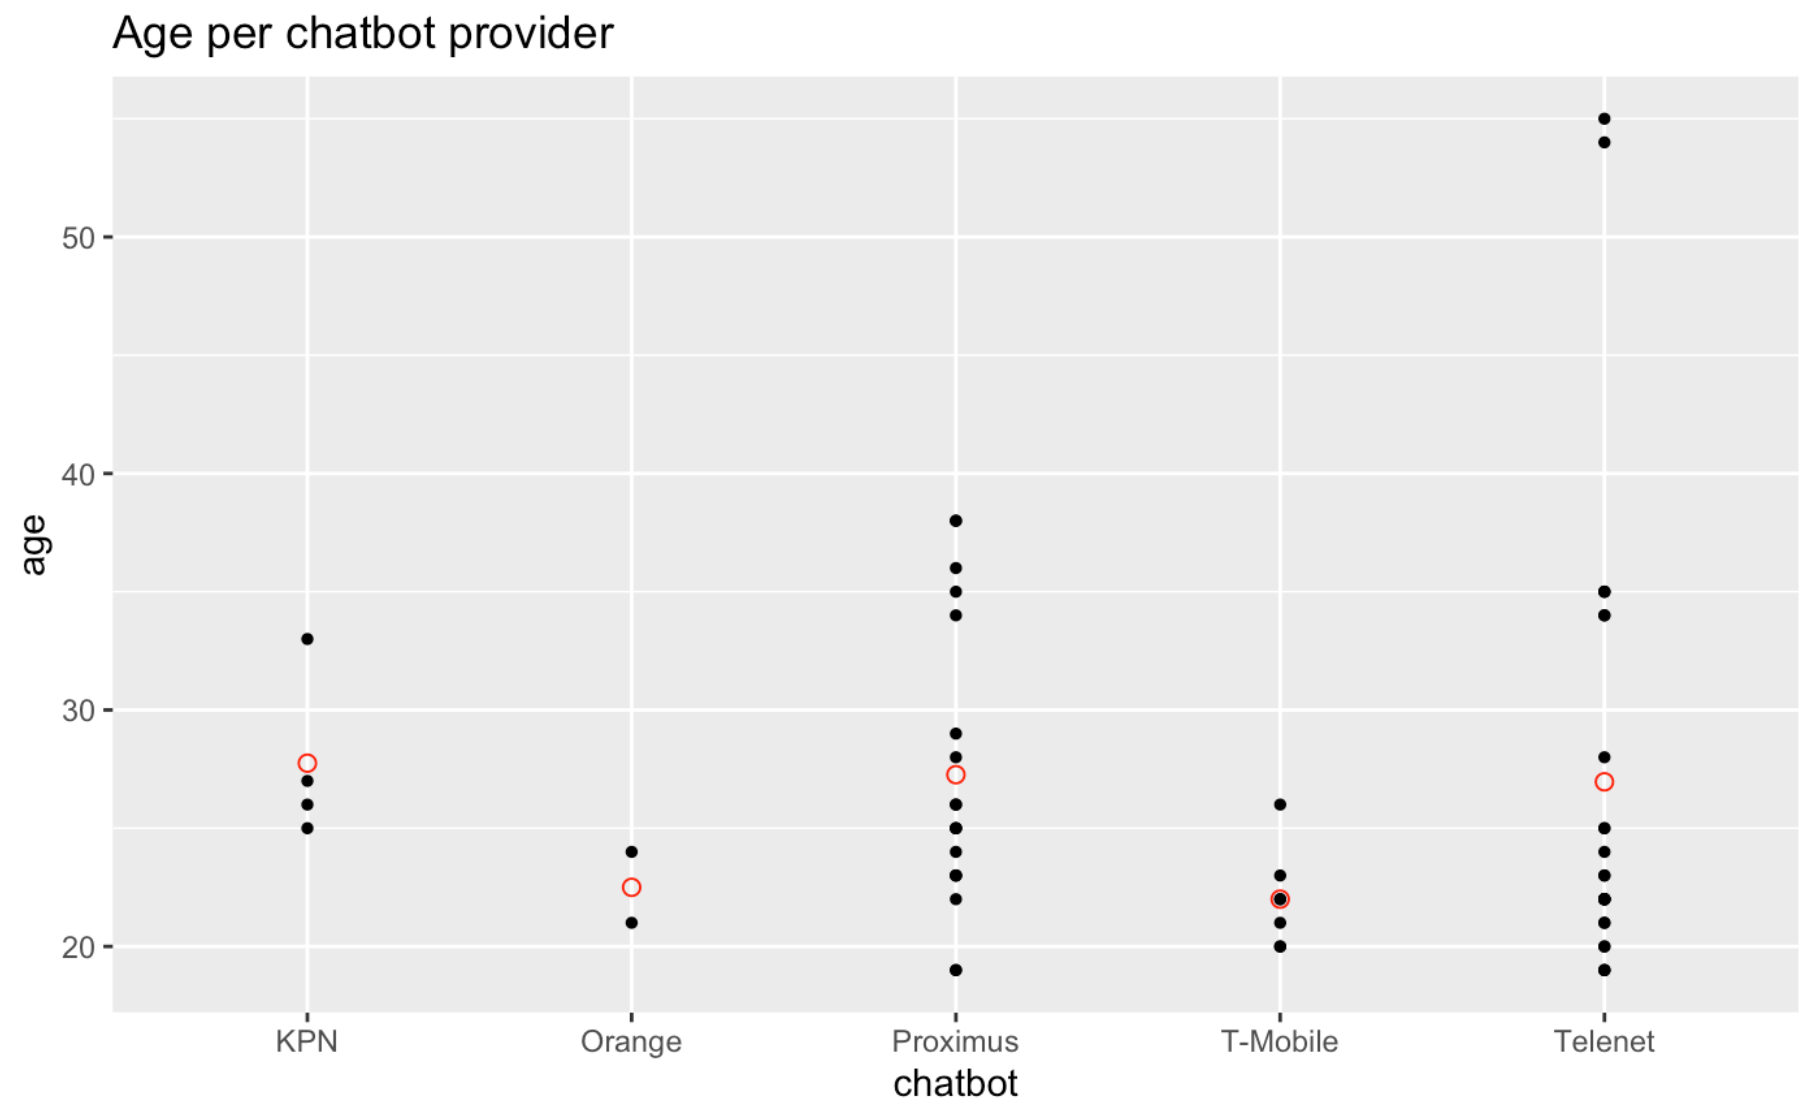
\includegraphics[width=\linewidth]{../LaTeX/Figures/Environments/AgePlot.png}
	\caption{The distribution of the age variable per chatbot provider.}\label{fig:agePlot}
	\endminipage\hfill
	\minipage{0.24\textwidth}
	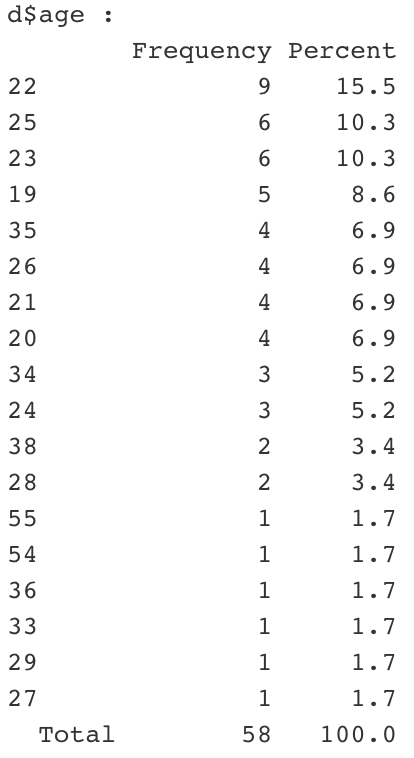
\includegraphics[width=\linewidth]{../LaTeX/Figures/Environments/AgeFreq.png}
	\caption{A frequency table of all the entries' ages.}\label{fig:ageFreq}
	\endminipage\hfill
\end{figure}


\subsubsection{Highest degree}
Looking at the acquired degrees of the respondents, the most common category is a master degree with 19 respondents, followed by an academic bachelor with 17 answers. Third comes high school with 12 (see Figure \ref{fig:degreePlot} and \ref{fig:degreeFreq}).
\begin{figure}[htb!]
	\minipage{0.55\textwidth}
	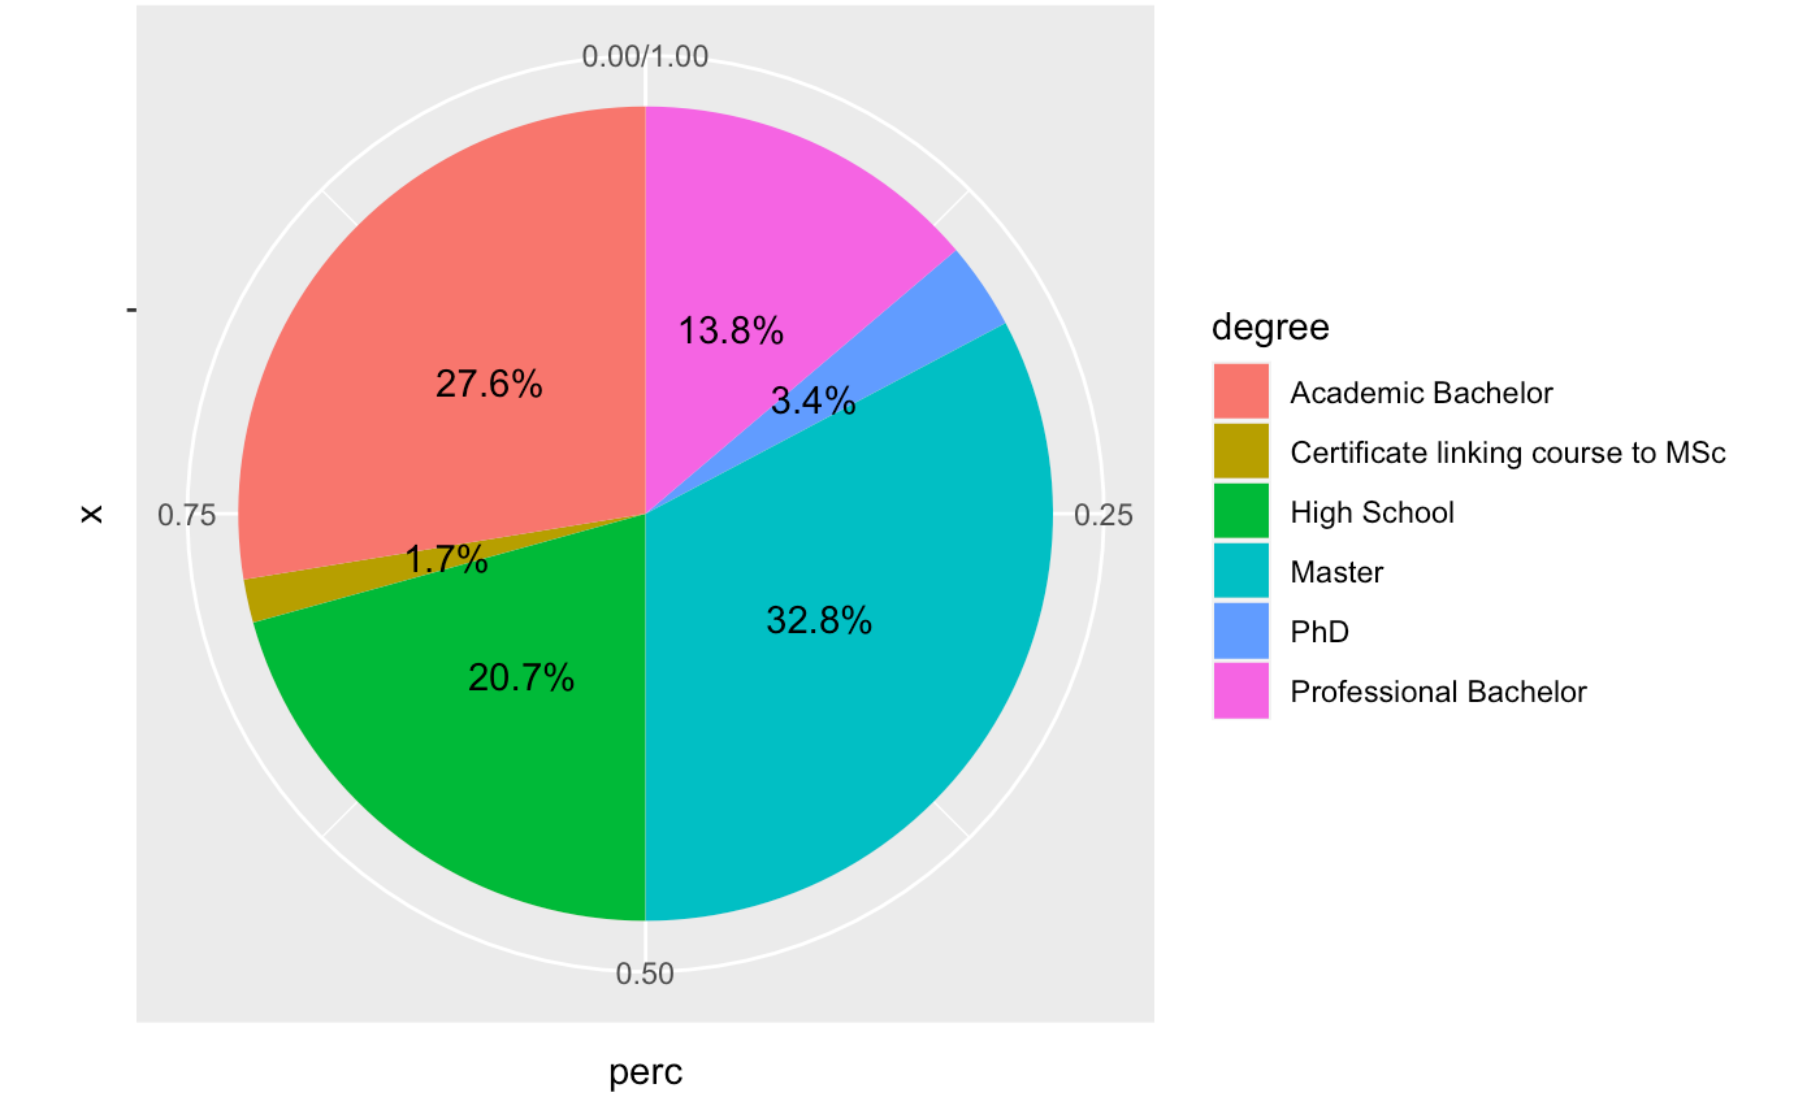
\includegraphics[width=\linewidth]{../LaTeX/Figures/Environments/DegreePlot.png}
	\caption{The distribution of the degree variable.}\label{fig:degreePlot}
	\endminipage\hfill
	\minipage{0.44\textwidth}
	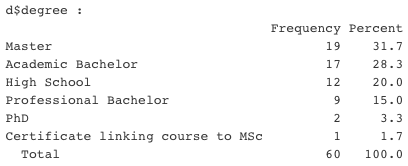
\includegraphics[width=\linewidth]{../LaTeX/Figures/Environments/DegreeFreq.png}
	\caption{A frequency table of all the entries' degrees.}\label{fig:degreeFreq}
	\endminipage\hfill
\end{figure}

\subsubsection{Gender}
There were 34 males who filled in the survey and 25 females. One person identified as non-binary (see Figure \ref{fig:genderPlot} and \ref{fig:genderFreq}).
\begin{figure}[!htb]
	\minipage{0.69\textwidth}
	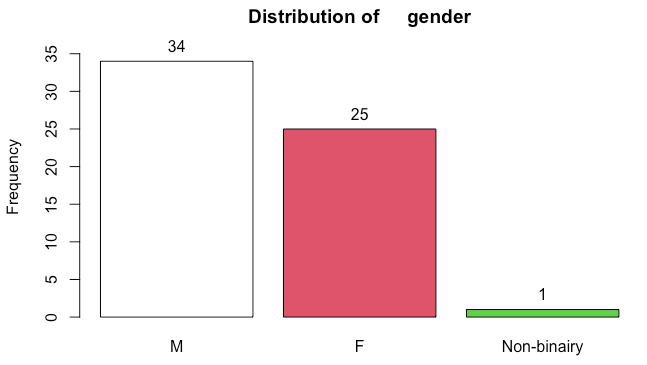
\includegraphics[width=\linewidth]{../LaTeX/Figures/Environments/GenderPlot.png}
	\caption{The distribution of the gender variable.}\label{fig:genderPlot}
	\endminipage\hfill
	\minipage{0.30\textwidth}
	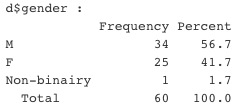
\includegraphics[width=\linewidth]{../LaTeX/Figures/Environments/GenderFreq.png}
	\caption{A frequency table of all the entries' genders.}\label{fig:genderFreq}
	\endminipage\hfill
\end{figure}

\subsubsection{Company of chatbot}
Telenet has the most respondents, followed by Proximus. The other chatbot providers are less represented (see Figure \ref{fig:chatbotPlot} and \ref{fig:chatbotFreq}).
\begin{figure}[!htb]
	\minipage{0.69\textwidth}
	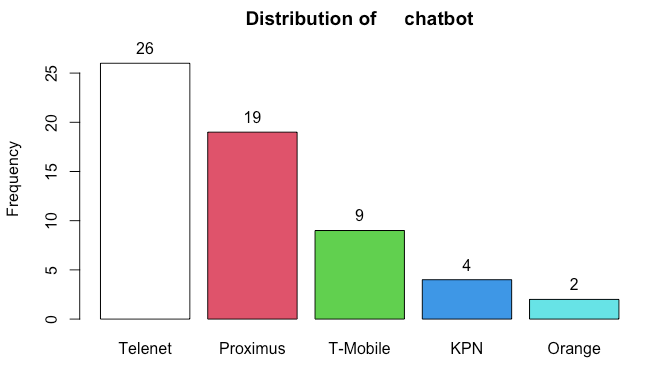
\includegraphics[width=\linewidth]{../LaTeX/Figures/Environments/ChatbotPlot.png}
	\caption{The distribution of the different chatbot providers and the amount of respondents for each provider.}\label{fig:chatbotPlot}
	\endminipage\hfill
	\minipage{0.30\textwidth}
	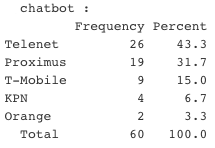
\includegraphics[width=\linewidth]{../LaTeX/Figures/Environments/ChatbotFreq.png}
	\caption{A frequency table of all the entries' used chatbots.}\label{fig:chatbotFreq}
	\endminipage\hfill
\end{figure}

\subsubsection{Used language}
Most users used Dutch as their preferred language of interaction which doesn't come as a surprise since this thesis focuses on the Flemish part of Belgium along with the Netherlands. Afterwards, English was the second most used language and French came last (see Figure \ref{fig:languagePlot} and \ref{fig:languageFreq}).

\begin{figure}[!htb]
	\minipage{0.69\textwidth}
	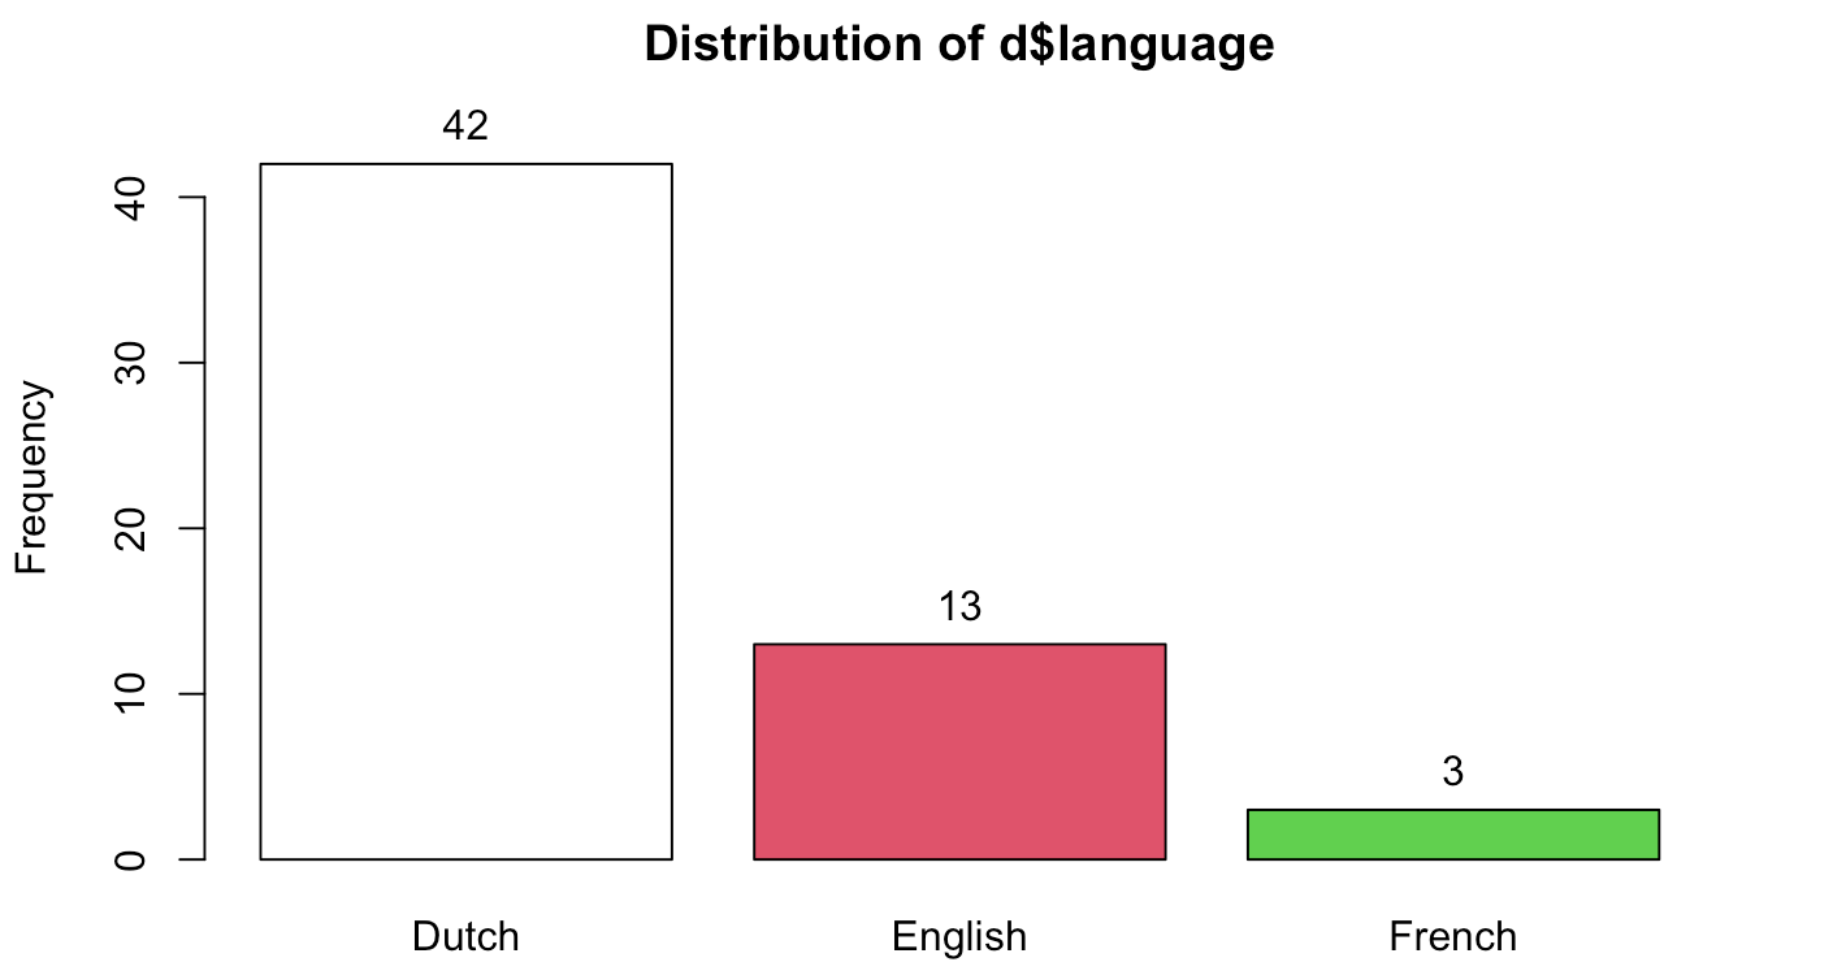
\includegraphics[width=\linewidth]{../LaTeX/Figures/Environments/LanguagePlot.png}
	\caption{The distribution of the language variable.}\label{fig:languagePlot}
	\endminipage\hfill
	\minipage{0.30\textwidth}
	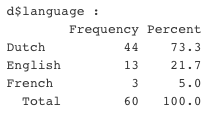
\includegraphics[width=\linewidth]{../LaTeX/Figures/Environments/LanguageFreq.png}
	\caption{A frequency table of all the entries' used languages.}\label{fig:languageFreq}
	\endminipage\hfill
\end{figure}

\subsubsection{Platform}
Most chatbots were used on the website of the provider themselves. Only a small percentage were used in app or via Facebook Messenger (see Figure \ref{fig:platformPlot} and \ref{fig:platformFreq}).

\begin{figure}[!htb]
	\minipage{0.69\textwidth}
	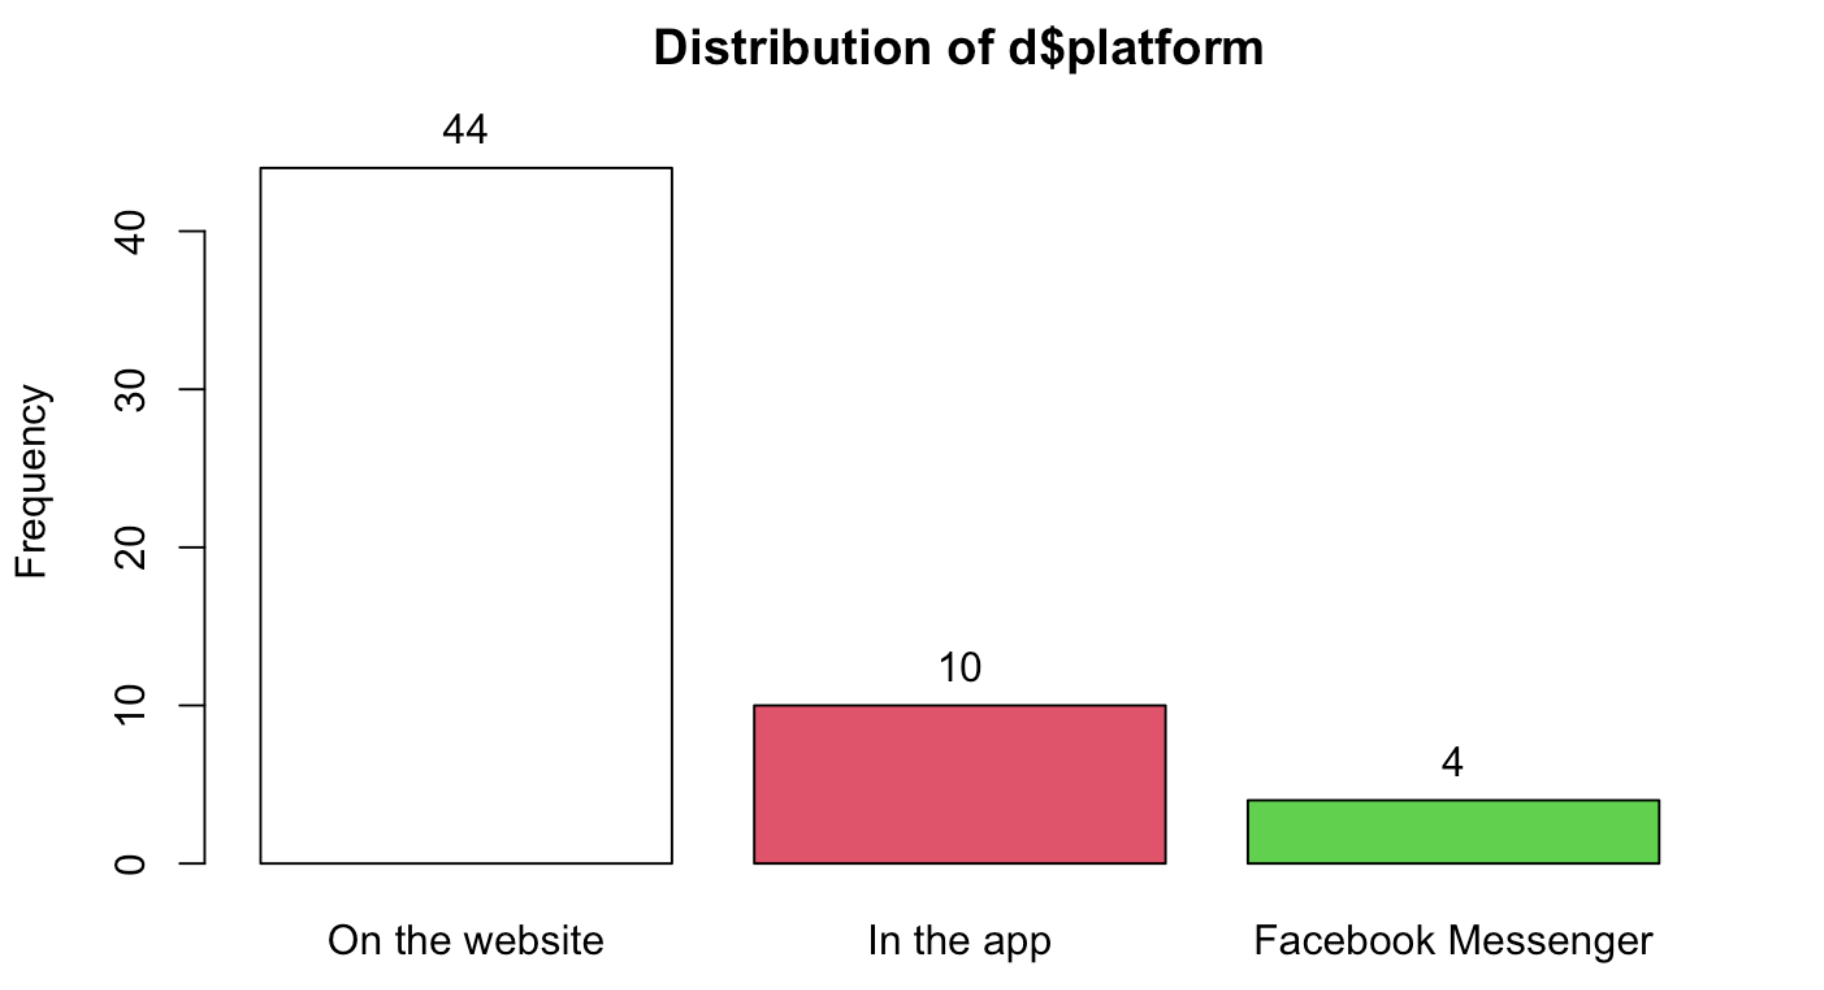
\includegraphics[width=\linewidth]{../LaTeX/Figures/Environments/PlatformPlot.png}
	\caption{The distribution of the platform variable.}\label{fig:platformPlot}
	\endminipage\hfill
	\minipage{0.30\textwidth}
	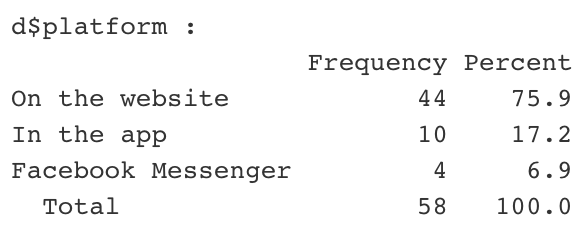
\includegraphics[width=\linewidth]{../LaTeX/Figures/Environments/PlatformFreq.png}
	\caption{A frequency table of all the entries' used platform to interact with the chatbot.}\label{fig:platformFreq}
	\endminipage\hfill
\end{figure}

\FloatBarrier
\subsection{Comparative Study}
\subsubsection{Business view (interviews)}
\begin{table}[htbp!]
	\centering
	\resizebox{\textwidth}{!}{%
		\begin{tabular}{|lllll|}
			\hline
			\multicolumn{5}{|c|}{\textbf{The current state of the customer service chatbot}} \\ \hline
			\multicolumn{1}{|l|}{} &
			\multicolumn{1}{l|}{Proximus} &
			\multicolumn{1}{l|}{Telenet} &
			\multicolumn{1}{l|}{T-Mobile} &
			KPN \\ \hline
			\multicolumn{1}{|l|}{\begin{tabular}[c]{@{}l@{}}Supported task \\ categories\end{tabular}} &
			\multicolumn{1}{l|}{FAQ} &
			\multicolumn{1}{l|}{FAQ} &
			\multicolumn{1}{l|}{\begin{tabular}[c]{@{}l@{}}FAQ, Sales (add-ons\\ like Deezer and \\ other video services)\end{tabular}} &
			FAQ \\ \hline
			\multicolumn{1}{|l|}{\begin{tabular}[c]{@{}l@{}}Supported \\ platforms\end{tabular}} &
			\multicolumn{1}{l|}{\begin{tabular}[c]{@{}l@{}}Website,\\ Messenger,\\ Proximus-app\end{tabular}} &
			\multicolumn{1}{l|}{Messenger} &
			\multicolumn{1}{l|}{Website and app} &
			Website and app\\ \hline
			\multicolumn{1}{|l|}{\begin{tabular}[c]{@{}l@{}}Supported \\ languages\end{tabular}} &
			\multicolumn{1}{l|}{\begin{tabular}[c]{@{}l@{}}Dutch, French,\\  English\end{tabular}} &
			\multicolumn{1}{l|}{\begin{tabular}[c]{@{}l@{}}Dutch, French,\\  English\end{tabular}} &
			\multicolumn{1}{l|}{Dutch} &
			Dutch \& English \\ \hline
			\multicolumn{1}{|l|}{\begin{tabular}[c]{@{}l@{}}Most common \\ user group\end{tabular}} &
			\multicolumn{1}{l|}{No information} &
			\multicolumn{1}{l|}{\begin{tabular}[c]{@{}l@{}}Younger people \\ and adults\\ (\textless{}= 40 years)\end{tabular}} &
			\multicolumn{1}{l|}{\begin{tabular}[c]{@{}l@{}}T-Mobile = younger \\ people\\ Tele2 = adults\end{tabular}} &
			Adults \\ \hline
			\multicolumn{1}{|l|}{\begin{tabular}[c]{@{}l@{}}Supported\\ questions\end{tabular}} &
			\multicolumn{1}{l|}{\begin{tabular}[c]{@{}l@{}}Yes/no, direct \\ \& vague \\ questions\end{tabular}} &
			\multicolumn{1}{l|}{\begin{tabular}[c]{@{}l@{}}Yes/no, direct \& \\ vague questions\end{tabular}} &
			\multicolumn{1}{l|}{\begin{tabular}[c]{@{}l@{}}Yes/no, direct \& \\ vague questions\end{tabular}} &
			\begin{tabular}[c]{@{}l@{}}Yes/no, direct \& \\ vague questions\end{tabular} \\ \hline
		\end{tabular}%
	}
	\caption{Overview of the current state of the customer service chatbots}
	\label{tab:currentState}
\end{table}
\ul{Supported task categories}\\
Later on, Proximus wants to develop their chatbot further into a proactive salesman with the aim of offering the best action or promotion. Complaints are forwarded by the bot directly to a live agent.\\
\break
Telenet used to have two chatbots, which were AskHugo and AskPlay. AskHugo was a bot that tried to convince customers to buy a Hugo subscription, AskPlay gave recommendations on which movies/series to watch. However, both chatbots were shut down because the \acrshort{roi} was too low.\\
\break
T-Mobile's\footnote{T-Mobile has merged with Tele2 since January 2019. The Tele2 brand has continued to exist and is now a part of T-Mobile. The management of Tele2's chatbot is also done by T-Mobile, these chatbots both use the same underlying system so both chatbots have the same operations.} chatbot can also guide the customer in choosing the right subscription or device. In this way, T-Mobile tries to keep as much "trivial" work away from the physical agents, because the explicit purchase of a specific subscription/device is only done through them. Complaints are partly handled by the bot, it will ask if the customer has already spoken to an employee about this, if this has happened, then the chatbot will give the procedure to file a complaint.\\
\break
At the chatbot of KPN, in case of complaints, the customer is redirected to a live chat; the bot's only function here is to gather customer information. Selling products and services is not offered in the bot because that is not yet technically possible, the bot only serves as a proactive assistant, if the customer has been in the shop for a while, the bot will ask the customer if he/she needs help.\\
\break
\ul{Supported platforms}\\
Telenet only offers its chatbot through Facebook Messenger, but this is integrated into their website and app. Communication through WhatsApp is also possible, but this only an auto-reply system. In the bot of T-Mobile, there is a difference between the platforms, on the website all services are offered, but in the application the chatbot is mainly focused on questions about mobile services. The bot recognises if the customer asks a question about another service, he will then be redirected. KPN basically only offers their chatbot on their website, but in the app it is also available through a web page built into the application. If the customer then consults the chatbot in the app, this is actually the chatbot on the website.\\
\break
\ul{Supported languages}\\
If the Proximus bot is addressed in a different language, the underlying \acrshort{ai} system will recognise that this language is not supported, and the bot will then choose to continue the conversation in English. When the bot of T-Mobile is used in another language, the customer is redirected to an agent. The English variant of KPN's bot has far fewer functions; it will redirect the customer to the right page on the website or continue the conversation with an agent. According to KPN, there is no need in the Netherlands to offer the chatbot in other languages (see Appendix A.4.1). \\
\break
\ul{Most common user group}\\
Proximus' broad customer base explains the big spread of its users, as they offer services that are used by young people, adults and the elderly. Telenet's most common user group can be explained because their bot can only be accessed via social media. T-Mobile only has insight into the bot users that have been identified (users who are logged in to their account). T-Mobile also anticipates on the age group by adjusting the chat style; in the Tele2 bot, more hashtags and emojis are used, in the T-Mobile bot this is more formal. KPN uses a neutral chat style in their bot, they don't want to address a specific age group.\\
\break
\ul{Supported type of questions}\\
For every bot except Telenet, the yes/no questions are supported. The treatment of the direct and vague is also in the same line in the different bots. Whenever a question is too vague, the bot will continue to ask until the various missing values have been filled in. In the T-Mobile bot, it was mentioned that there is a limit to the number of times that a certain missing value can be queried. If the bot needs to re-ask a certain number of times before it can provide an answer, the chat will be redirected to a live agent to avoid user frustration. To address the same issue, KPN is using a button where the user can indicate whether they mean something different or have a different question. Telenet's chatbot can't interpret anything, you have to work with the buttons provided by the chatbot.\\
\begin{table}[htbp!]
	\centering
	\resizebox{\textwidth}{!}{%
		\begin{tabular}{|lllll|}
			\hline
			\multicolumn{5}{|c|}{\textbf{The benefits that the company derives from the presence of the chatbot}} \\ \hline
			\multicolumn{1}{|l|}{} &
			\multicolumn{1}{l|}{Proximus} &
			\multicolumn{1}{l|}{Telenet} &
			\multicolumn{1}{l|}{T-Mobile} &
			KPN \\ \hline
			\multicolumn{1}{|l|}{\begin{tabular}[c]{@{}l@{}}Supported\\ services\end{tabular}} &
			\multicolumn{1}{l|}{\begin{tabular}[c]{@{}l@{}}- Retrieve pincode\\ - Outstanding\\ invoice amount\\ - Retrieve status\\ of your subscription\\ and services\end{tabular}} &
			\multicolumn{1}{l|}{- Only support} &
			\multicolumn{1}{l|}{\begin{tabular}[c]{@{}l@{}}- Retrieve customer\\ information (client\\ number, puk code\\ , etc.)\\ -Adjust personal\\ settings (e.g.\\ deactivate extra\\ costs if a service \\ number calls)\\ - Buy add-ons (e.g.\\ mobile data bundle)\\  - Manages \\ workforce of agents\end{tabular}} &
			\begin{tabular}[c]{@{}l@{}}- Preparer for\\ agents (making\\ their conversation\\ shorter)\\ - Guide to lead\\ customer to right\\ place on website\end{tabular} \\ \hline
			\multicolumn{1}{|l|}{\begin{tabular}[c]{@{}l@{}}Reduction of\\ employee\\ workload\end{tabular}} &
			\multicolumn{1}{l|}{\begin{tabular}[c]{@{}l@{}}No data because of\\ confidential \\ information\end{tabular}} &
			\multicolumn{1}{l|}{\begin{tabular}[c]{@{}l@{}}No data because\\ of confidential\\ information\end{tabular}} &
			\multicolumn{1}{l|}{\begin{tabular}[c]{@{}l@{}}25\% of the question\\ can not be answered\\ in the chatbot\end{tabular}} &
			\begin{tabular}[c]{@{}l@{}}The chatbot takes\\ over 25\% of the\\ work\end{tabular} \\ \hline
			\multicolumn{1}{|l|}{\begin{tabular}[c]{@{}l@{}}Customer's\\ willingness to\\ use chatbot\end{tabular}} &
			\multicolumn{1}{l|}{\begin{tabular}[c]{@{}l@{}}No data because of \\ confidential \\ information\end{tabular}} &
			\multicolumn{1}{l|}{\begin{tabular}[c]{@{}l@{}}65\% of the users\\ are willing to go\\ through the\\ whole flow\end{tabular}} &
			\multicolumn{1}{l|}{No data available} &
			\begin{tabular}[c]{@{}l@{}}20\% of the users\\ are willing to\\ directly speak to\\ an agent\end{tabular} \\ \hline
			\multicolumn{1}{|l|}{\begin{tabular}[c]{@{}l@{}}Negative\\ influences\end{tabular}} &
			\multicolumn{1}{l|}{\begin{tabular}[c]{@{}l@{}}- Frustration\\ because of bad \\ experience and\\ prejudice\end{tabular}} &
			\multicolumn{1}{l|}{\begin{tabular}[c]{@{}l@{}}- Frustration\\ because of the\\ change to a new\\ platform\end{tabular}} &
			\multicolumn{1}{l|}{\begin{tabular}[c]{@{}l@{}}- Frustration because\\ of bad experience\\ and prejudice\end{tabular}} &
			\begin{tabular}[c]{@{}l@{}}No data available\\ because of \\ confidential\\ information\end{tabular} \\ \hline
		\end{tabular}%
	}
	\caption{Overview of the benefits that companies derive from the presence of the chatbot}
	\label{tab:benefits}
\end{table}
\break
\ul{Supported services}\\
The purpose of Proximus' chatbot is to offer solutions, not instructions such as "for that task, you can go to this web page". At T-Mobile, the sales contracts are not handled in the chatbot because the sales department does not want it to deal with their sales strategies.\\
\break
\ul{Reduction of employee workload}\\
Proximus said that not everything in customer service was covered, so for some issues customers are redirected to an employee. The chatbot of Telenet reduces the workload, but the impact is still limited. T-Mobile's numbers can be explained by poor language use by the customer or the complexity and specificity of the question. The results of KPN's chatbot can be explained as the bot does not have enough knowledge to answer the question; for some services, such as cancelling subscriptions or complaints, the customer is always referred to a member of staff. It is estimated that about a quarter (25\%) of the agents' work is taken over by the chatbot.\\
\break
\ul{Customer's willingness to use chatbot}\\
The willingness to use the chatbot is examined by each company on the basis of feedback, with feedback one must also take into account voluntary response bias, customers who are not satisfied with certain services will give feedback more quickly than others.\\
\break
At Proximus the satisfaction lies in both camps, there are customers who are very satisfied with the chatbot, but there are also customers who think it is very bad.\\ 
\break
In the bot of Telenet, the reason why the remaining 30-35\% drop out is explained by a bad previous experience with a similar chatbot.\\ 
\break
T-Mobile asks their customers for feedback after a conversation with a chatbot. Analyses showed that the majority of responses ultimately had to call an agent to solve their problem. What T-Mobile also does to gain more insight into their customers is to work with personas. These are linked to possible customer profiles where they map out the corresponding requirements of the customer.\\ 
\break
At KPN, the number of direct calls (telephone) to a physical agent would be up higher, to an order of about 10, than with the chatbot. This means that there are 10 times more calls than chats.\\
\break
\ul{Negative influences}\\
Proximus sees mainly negative influences in the form of customers who are frustrated. The frustration arises when the chatbot does not understand the customer properly and goes the wrong way, this demotivates the customer to reuse the bot. Customers who are already frustrated by services that don't work properly should be taken into account, if these customers then come into contact with a chatbot it won't help their mood.\\
\break
Telenet experiences similar scenarios, it was further explained that it can be frustrating for customers to switch to a new platform, namely from 100\% helpdesk to a chatbot. According to Ms Portolani, some customers expect that a chatbot can interpret in the same way as an agent.\\
\break
T-Mobile has the same negative aspects as Proximus, they try to solve this by applying a limited form of sentiment analysis. If they measure that a customer is communicating in a frustrated way, they will forward this customer to an agent.\\
\break
At KPN, different metrics are used. For instance, the \gls{nps} measures the extent to which customers would recommend the company to acquaintances. The \acrshort{ces} measures how much effort it took to find the answer to the question. The final metric measured is the \acrshort{gcr}, which tells more about how well the customer was helped. The results of these metrics were not shared due to confidential information.\\
\break
\begin{longtable}[c]{|lllll|}
	\hline
	\multicolumn{5}{|c|}{\textbf{The business value (revenue, reduced costs) realised by the chatbot}} \\ \hline
	\endhead
	%
	\multicolumn{1}{|l|}{} &
	\multicolumn{1}{l|}{Proximus} &
	\multicolumn{1}{l|}{Telenet} &
	\multicolumn{1}{l|}{T-Mobile} &
	KPN \\ \hline
	\multicolumn{1}{|l|}{\begin{tabular}[c]{@{}l@{}}Increased \\ revenue\end{tabular}} &
	\multicolumn{1}{l|}{\begin{tabular}[c]{@{}l@{}}- No direct \\ revenue because \\ ROI is not\\ yet determined\\ - Chatbot directly\\ ensures they have\\ to spend less on\\ human helpdesk\\ agents\end{tabular}} &
	\multicolumn{1}{l|}{\begin{tabular}[c]{@{}l@{}}- No picture of\\ how much extra\\ revenue\\ - They have\\ fewer costs to\\ spent on\\ physical agents\end{tabular}} &
	\multicolumn{1}{l|}{\begin{tabular}[c]{@{}l@{}}- No concrete\\ figures, because\\ it's not measured\\ - Extra business\\ value is created\\ because fewer \\ costs to spent \\ on physical agents\end{tabular}} &
	\begin{tabular}[c]{@{}l@{}}- No concrete\\ figures, because \\ it'snot measured\\ - Extra business\\  value is created\\ because fewer \\ costs to spent on \\ physical agents\end{tabular} \\ \hline
	\multicolumn{1}{|l|}{Availability} &
	\multicolumn{1}{l|}{\begin{tabular}[c]{@{}l@{}}- 24/7 available\\ - Follow-up on \\ social media is \\ always possible\\ - Follow-up on the\\ website and in the\\ app is only \\ possible if user is \\ authenticated\end{tabular}} &
	\multicolumn{1}{l|}{\begin{tabular}[c]{@{}l@{}}- 24/7 available\\ - Follow-up is\\ always possible\\ because they\\ only use social\\ media\end{tabular}} &
	\multicolumn{1}{l|}{\begin{tabular}[c]{@{}l@{}}- 24/7 available\\ - Conversation is \\ not tracked, so the \\ customer will have \\ to consult the \\ chatbot again \\ during opening \\ hours if the \\ question cannot\\  be answered by \\ the chatbot\end{tabular}} &
	\begin{tabular}[c]{@{}l@{}}- 24/7 available\\ - Conversation is \\ not tracked, so \\ the customer will \\ have to consult \\ the chatbot again \\ during opening \\ hours if the \\ question cannot \\ be answered by \\ the chatbot\end{tabular} \\ \hline
	\multicolumn{1}{|l|}{\begin{tabular}[c]{@{}l@{}}Costs \& \\ biggest \\ cost items\end{tabular}} &
	\multicolumn{1}{l|}{\begin{tabular}[c]{@{}l@{}}- Costs depend\\ mainly on the\\ platform and the\\ size (number of\\ questions / \\ scenarios the bot \\ can handle)\\  of the chatbot\\ Biggest cost \\ items:\\ - Per incoming\\ chat, the NLP is\\ triggered, this \\ costs around \\ 1cent/chat\\ - The team behind\\ the chatbot, this \\ consists of in-\\ house frontend \\ and backend \\ developers,\\ configuration / \\ conversation \\ designers(via \\ consultancy and \\ cost about €400/\\ day) and an \\ engineer that \\ trains and corrects \\ the NLP\end{tabular}} &
	\multicolumn{1}{l|}{\begin{tabular}[c]{@{}l@{}}- They use a\\ pay-as-you-go\\ service, specific\\ costs could not\\ be shared\\ because of\\ confidential\\ information\\ Biggest cost\\ items:\\ - Hosting of the\\ chatbot\\ - Team behind\\ the development,\\ it consists of a\\ data scientist,\\ developer,\\ functional analyst\\ and a product\\ owner. It was\\ reported that \\ most of the costs \\ goes\\ to the team.\end{tabular}} &
	\multicolumn{1}{l|}{\begin{tabular}[c]{@{}l@{}}Specific costs could\\ not be shared because\\ of confidential \\ information\\ Biggest cost items:\\ - They have a\\ significant amount of\\ running costs because\\ the run their chatbot\\ in the cloud\\ - They use \\ Dialogflow (Google),\\  this tool contains \\ a CMS and\\ you can apply AI in\\ it\\ - Running costs\\ consist of \\ classification API, \\ database operations\\ and running the \\ engines to keep \\ everything working\\ - Largest part of the \\ costs go to the team \\ behind the bot, it \\ consists of two \\ developers, \\ full-stack developers \\ from India (quantity \\ unknown),\\ two AI trainers and\\ two conversation\\ designers\end{tabular}} &
	\begin{tabular}[c]{@{}l@{}}- They buy the \\ chatbot services \\ from another \\ company\\ -No specific data \\ on the costs could \\ be shared because \\ of confidential\\ information\\ Biggest cost items:\\ - The price they \\ pay\\ to the company\\ that created \\ and hosts the \\ chatbot\\ - Two teams that \\ work on the bot (\\ conversational\\ designers, product\\ owners, ...)\end{tabular} \\ \hline
	\caption{Overview of the business value (revenue, reduced costs) that are realised by the chatbots}
	\label{tab:businessValue}\\
\end{longtable}
Every chatbot that was questioned is available 24/7, but there is a difference in the handling of questions that cannot be solved by the chatbot during non-opening hours.\\
\break
\begin{longtable}[c]{|lllll|}
	\hline
	\multicolumn{5}{|c|}{\textbf{The future vision of the chatbot}} \\ \hline
	\endhead
	%
	\multicolumn{1}{|l|}{} &
	\multicolumn{1}{l|}{Proximus} &
	\multicolumn{1}{l|}{Telenet} &
	\multicolumn{1}{l|}{T-Mobile} &
	KPN \\ \hline
	\multicolumn{1}{|l|}{\begin{tabular}[c]{@{}l@{}}Focal points\\ for the \\ future\end{tabular}} &
	\multicolumn{1}{l|}{\begin{tabular}[c]{@{}l@{}}- Future view was\\ mostly confidential\\ - In general, they\\ are looking to \\ automate their \\ services and be \\ stronger in terms \\ of conversation\\ - Are looking\\ further into voice\\ control (next\\ channel they will\\ capetilise on\\ - Reducing the\\ buttons in their \\ bot, goal is to be \\ as conversational \\ as possible\\ - Are looking into\\ computer vision*\\ - In the long term,\\ they want to\\ integrate the bot\\ with Alexa, \\ Google Home, \\ etc.\end{tabular}} &
	\multicolumn{1}{l|}{\begin{tabular}[c]{@{}l@{}}- Are currently\\ working on a \\ platform in \\ which the \\ chatbot can\\ take more tasks\\ and answer \\ questions\\ independently\\ - They want to\\ add sentiment\\ analysis\\ - Branding the\\ new chatbot to\\ make it known\\ to their future\\ users\\ - They want to\\ add text\\ prediction to the\\ tool of the \\ human agents*\end{tabular}} &
	\multicolumn{1}{l|}{\begin{tabular}[c]{@{}l@{}}- They want to offer\\ the chatbot more\\ proactively on the\\ website\\ - Making the chatbot\\ available in more \\ languages with a \\ translate API (both\\ parties can then use\\ the bot in their own\\ language)\\ - Add asynchronous\\ messaging*\end{tabular}} &
	\begin{tabular}[c]{@{}l@{}}- Making the bot\\ available in more\\ places (presence\\ on social media\\ as Facebook \\ Messenger and \\ WhatsApp)\\ - Harmonise the\\ entire \\ communication \\ with the customer\\ (if the customer \\ send them via \\ WhatsApp,\\ they want to be \\ aware of this \\ conversation\\ if the customer\\ contacts them via \\ another platform\end{tabular} \\ \hline
	\multicolumn{1}{|l|}{\begin{tabular}[c]{@{}l@{}}Additional\\ chatbot-\\ features\end{tabular}} &
	\multicolumn{1}{l|}{\begin{tabular}[c]{@{}l@{}}Uses AI to classify\\ the question or \\ statement, \\ once this \\ is classified a \\ rules-based \\ approach is used\end{tabular}} &
	\multicolumn{1}{l|}{\begin{tabular}[c]{@{}l@{}}Only uses a \\ rules-based \\ approach\end{tabular}} &
	\multicolumn{1}{l|}{\begin{tabular}[c]{@{}l@{}}Uses AI to classify\\ the question or \\ statement, once this\\ is classified a \\ rules-based approach\\ is used\end{tabular}} &
	\begin{tabular}[c]{@{}l@{}}Uses AI to classify\\ the question or \\ statement, once this\\ is classified a \\ rules-based \\ approach is used\end{tabular} \\ \hline
	\multicolumn{1}{|l|}{\begin{tabular}[c]{@{}l@{}}Source of\\ knowledge\\ to improve\\ chatbot\end{tabular}} &
	\multicolumn{1}{l|}{\begin{tabular}[c]{@{}l@{}}They use \\ benchmarking,\\ marketing studies,\\ check-ins with \\ other companies, \\ research in papers\\ and participation\\ in many \\ conferences \\ to gather extra \\ information on\\ relevant topics\end{tabular}} &
	\multicolumn{1}{l|}{\begin{tabular}[c]{@{}l@{}}- Are using data\\ analysis\\ - They look at\\ the experience \\ of their agents\end{tabular}} &
	\multicolumn{1}{l|}{\begin{tabular}[c]{@{}l@{}}- Uses data analysis,\\ each conversation is\\ logged and they can\\ query to gather \\ information on \\ specific topics\\ - Customer feedback\\ is taken into account,\\ in the conversations\\ that went well, they\\ take the common\\ features and use \\ them to standardize \\ this in the \\ conversation design,\\ for the bad\\ conversations, they\\ look for aspects that\\ they can further \\ improve\end{tabular}} &
	\begin{tabular}[c]{@{}l@{}}- Main focus on \\ data analysis to \\ continuously \\ review how they \\ can improve the \\ conversations\end{tabular} \\ \hline
	\caption{Overview of the future vision of the different chatbots}
	\label{tab:futureVision}\\
\end{longtable}
Proximus is looking into integrating computer vision, for example, if a picture of an invoice is sent in the bot, it can automatically recognise the different elements.\\
\break
Telenet is focusing on automating certain things the agents work with, they want to add text prediction so when the agent starts typing they will automatically prefill things so the agent does not have to type everything themselves.\\
\break
T-Mobile is working on adding asynchronous messaging, which means that if it is necessary to chat with an agent, no synchronous connection is needed, and the flow of the chat will continue exactly as it started with the chatbot. The latter will also ensure that customers do not need to send their question again if they have consulted the chatbot outside of helpdesk opening hours.

\subsubsection{Customer view (survey)}
In this part, a comparison will be drawn between the different companies in accordance to the business interview and gathered data in the survey. Because Orange, T-Mobile and KPN did not get enough responses to be viewed on their own, these three providers will be grouped together in the group 'others'.\\
\break
Next up, the task categories. Because the interview showed that chatbots are not yet equipped to deal with both complaints as well as sales questions, these two will not be included in the comparative study. For personal questions, there are not enough entries to view this as it is own category. The focus will therefor be on FAQ questions.\\
\break
All graphs will be presented as follows: Telenet on the left, Proximus in the middle and the 'others' on the right.\\
\break
\ul{Attribute 1: Execute the requested task}\\
\break
Looking at how the chatbots performed when solving a task, both Telenet and Proximus seem to have a split customer base where around 50\% is happy and 50\% is not. When looking at the others, there is a clear happiness about how the chatbot performed.\\
\begin{figure}[!htb]
	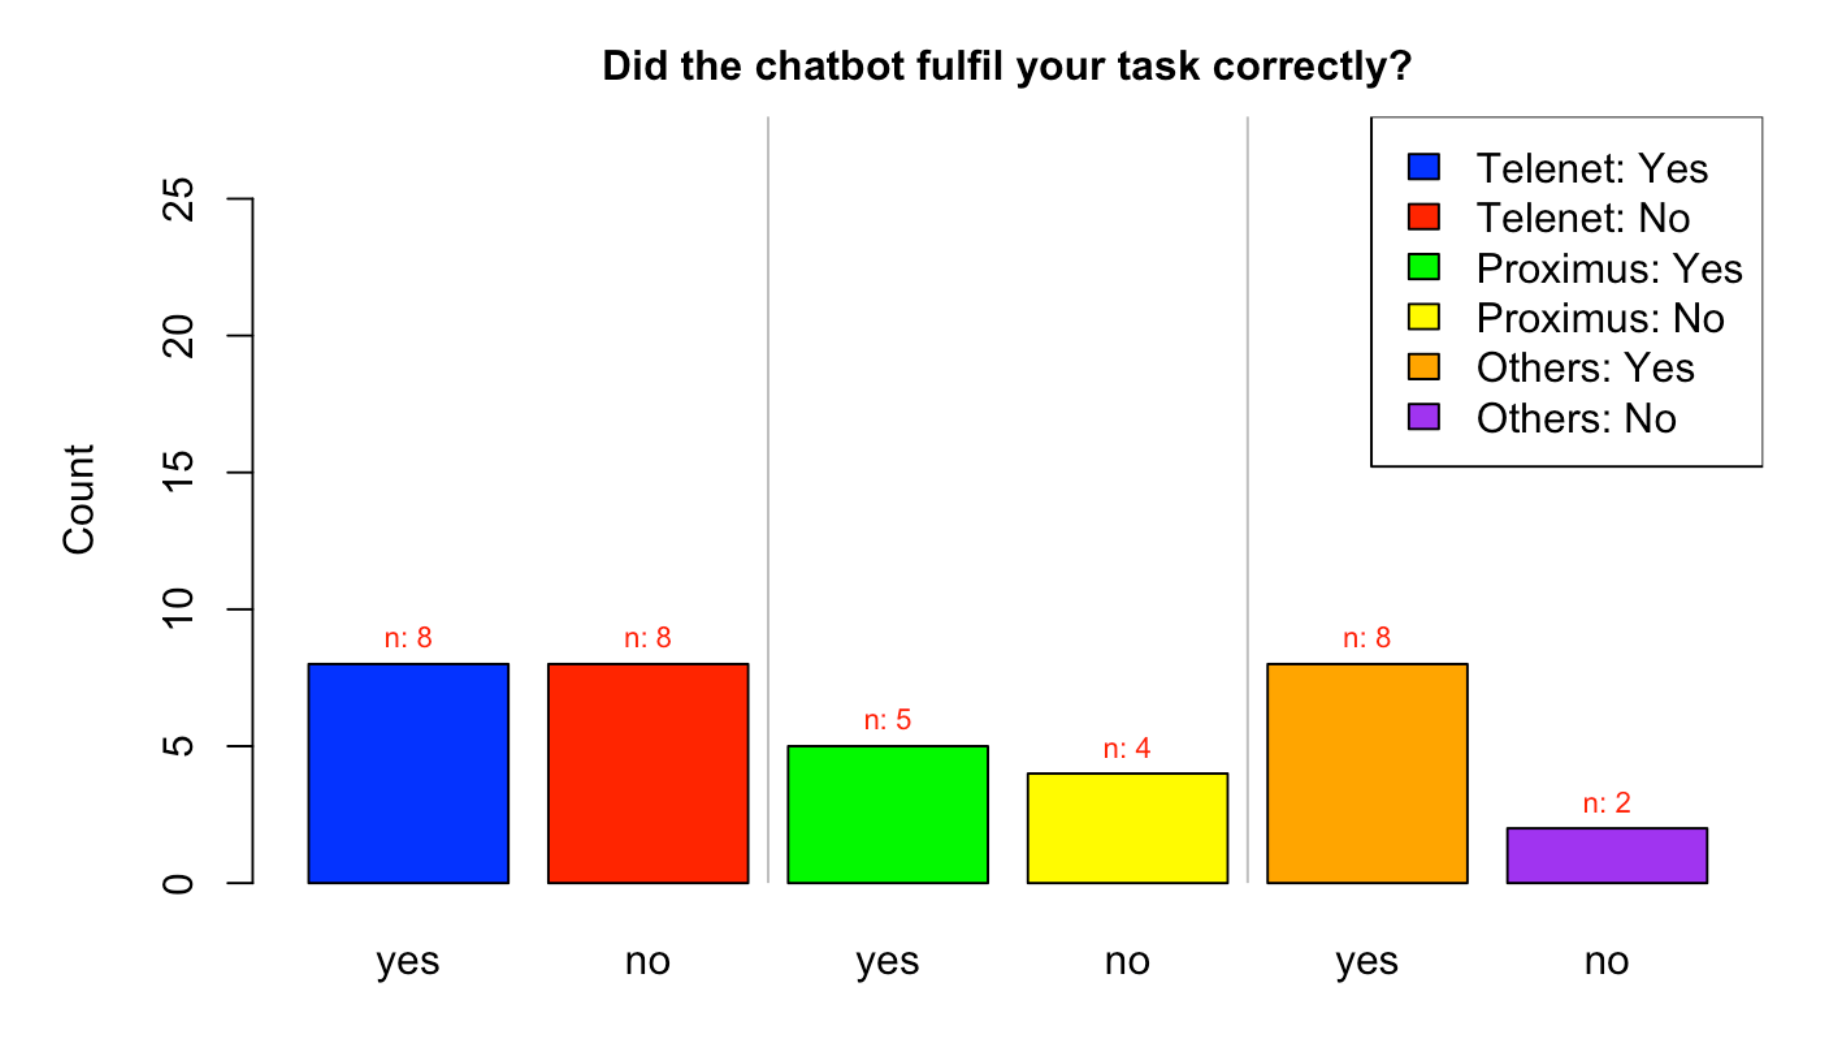
\includegraphics[width=\linewidth, scale=0.5]{../LaTeX/Figures/Comparative/Q1.png}
	\caption{Responses about the functional question for \acrshort{qa} 1, question 1.}\label{fig:Q1}
\end{figure}
Looking at the counter part of the previous question, there is even more discontent with Proximus. The results for Telenet and the others confirm the previous findings.
\begin{figure}[!htb]
	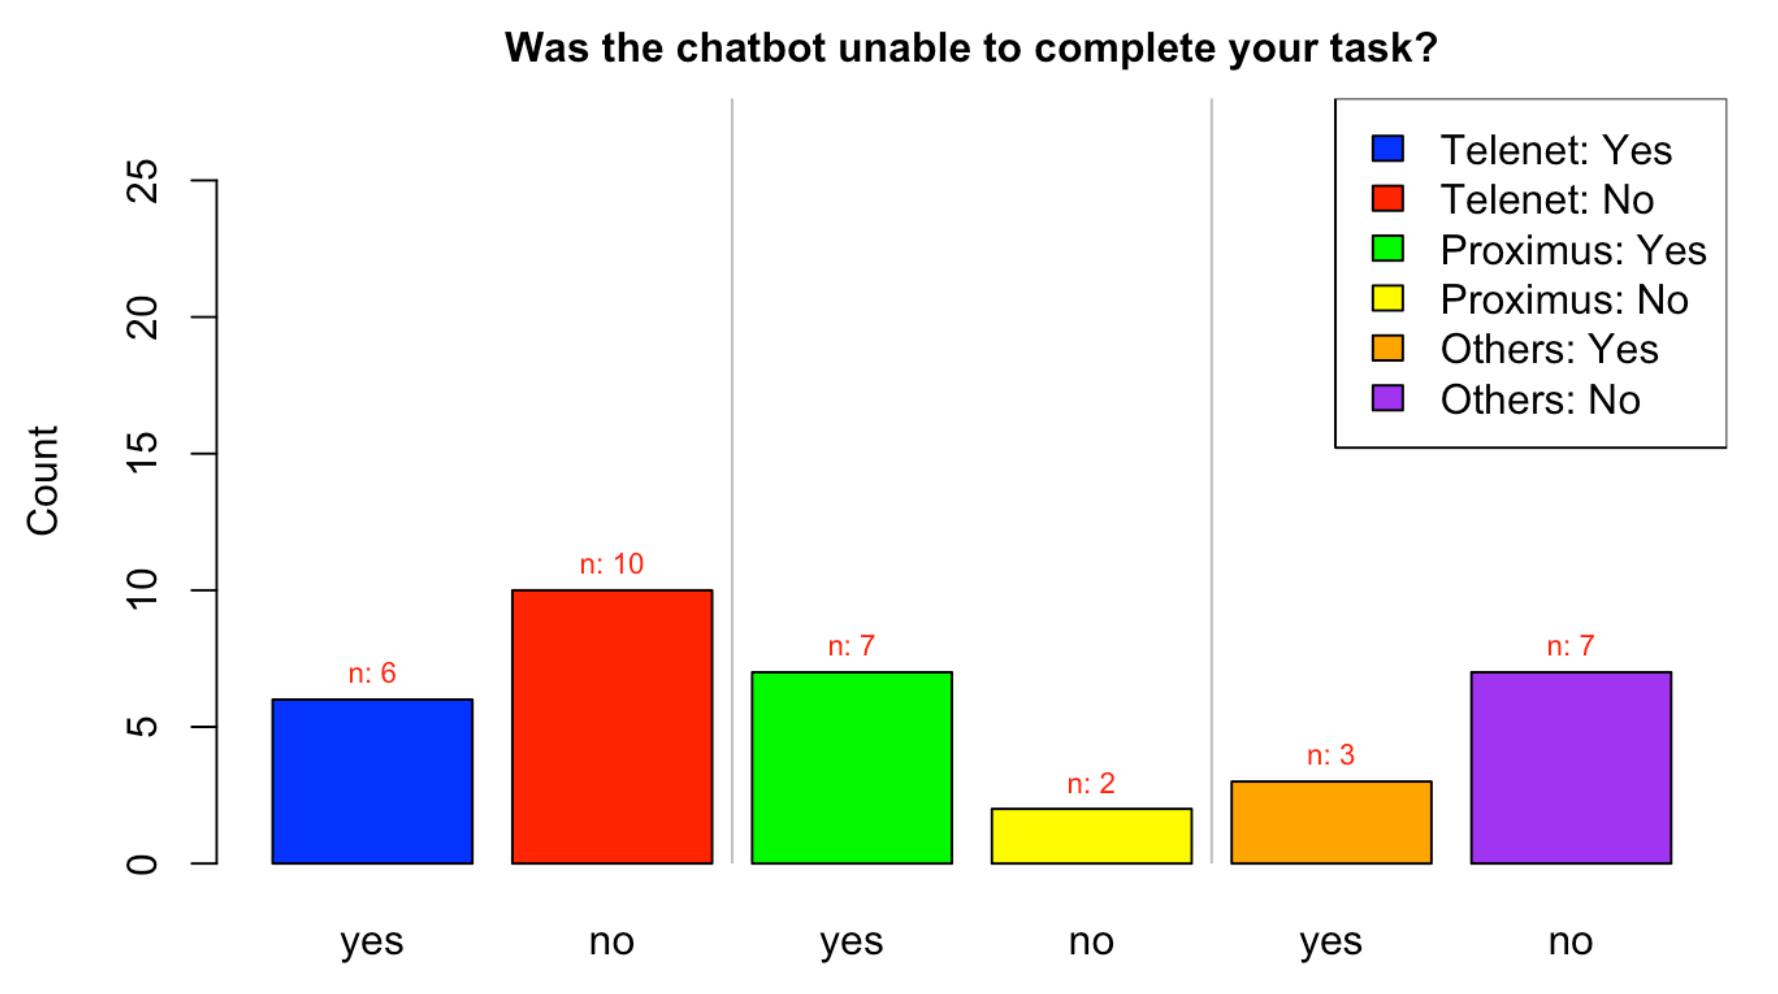
\includegraphics[width=\linewidth, scale=0.5]{../LaTeX/Figures/Comparative/DQ1.png}
	\caption{Responses about the dysfunctional question for \acrshort{qa} 1, question 1.}\label{fig:DQ1}
\end{figure}
\break
Looking at the results whether the chatbot needed help from an agent to complete it's task, there again is almost a 50-50 split for Telenet and Proximus whereas the others did better again.\\
\begin{figure}[!htb]
	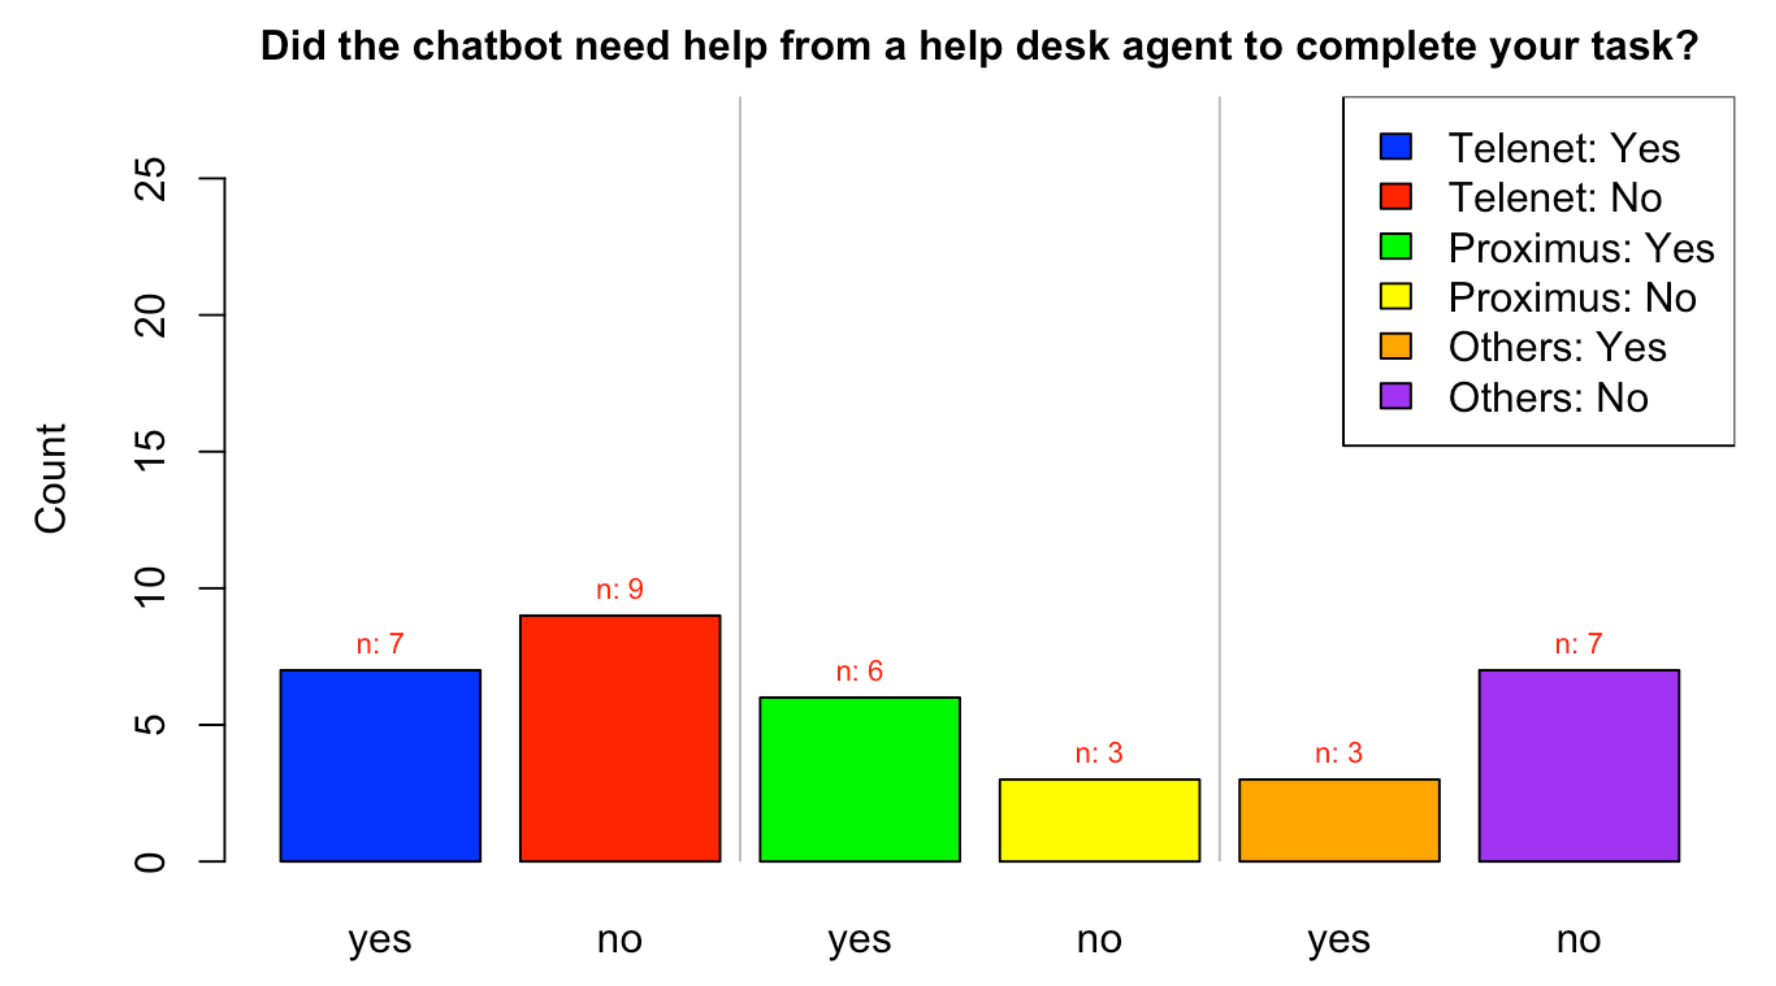
\includegraphics[width=\linewidth, scale=0.5]{../LaTeX/Figures/Comparative/Q1b.png}
	\caption{Responses about the functional question for \acrshort{qa} 1, question 2.}\label{fig:Q1b}
\end{figure}
The dysfunctional version of the previous question confirms these findings.\\
\begin{figure}[!htb]
	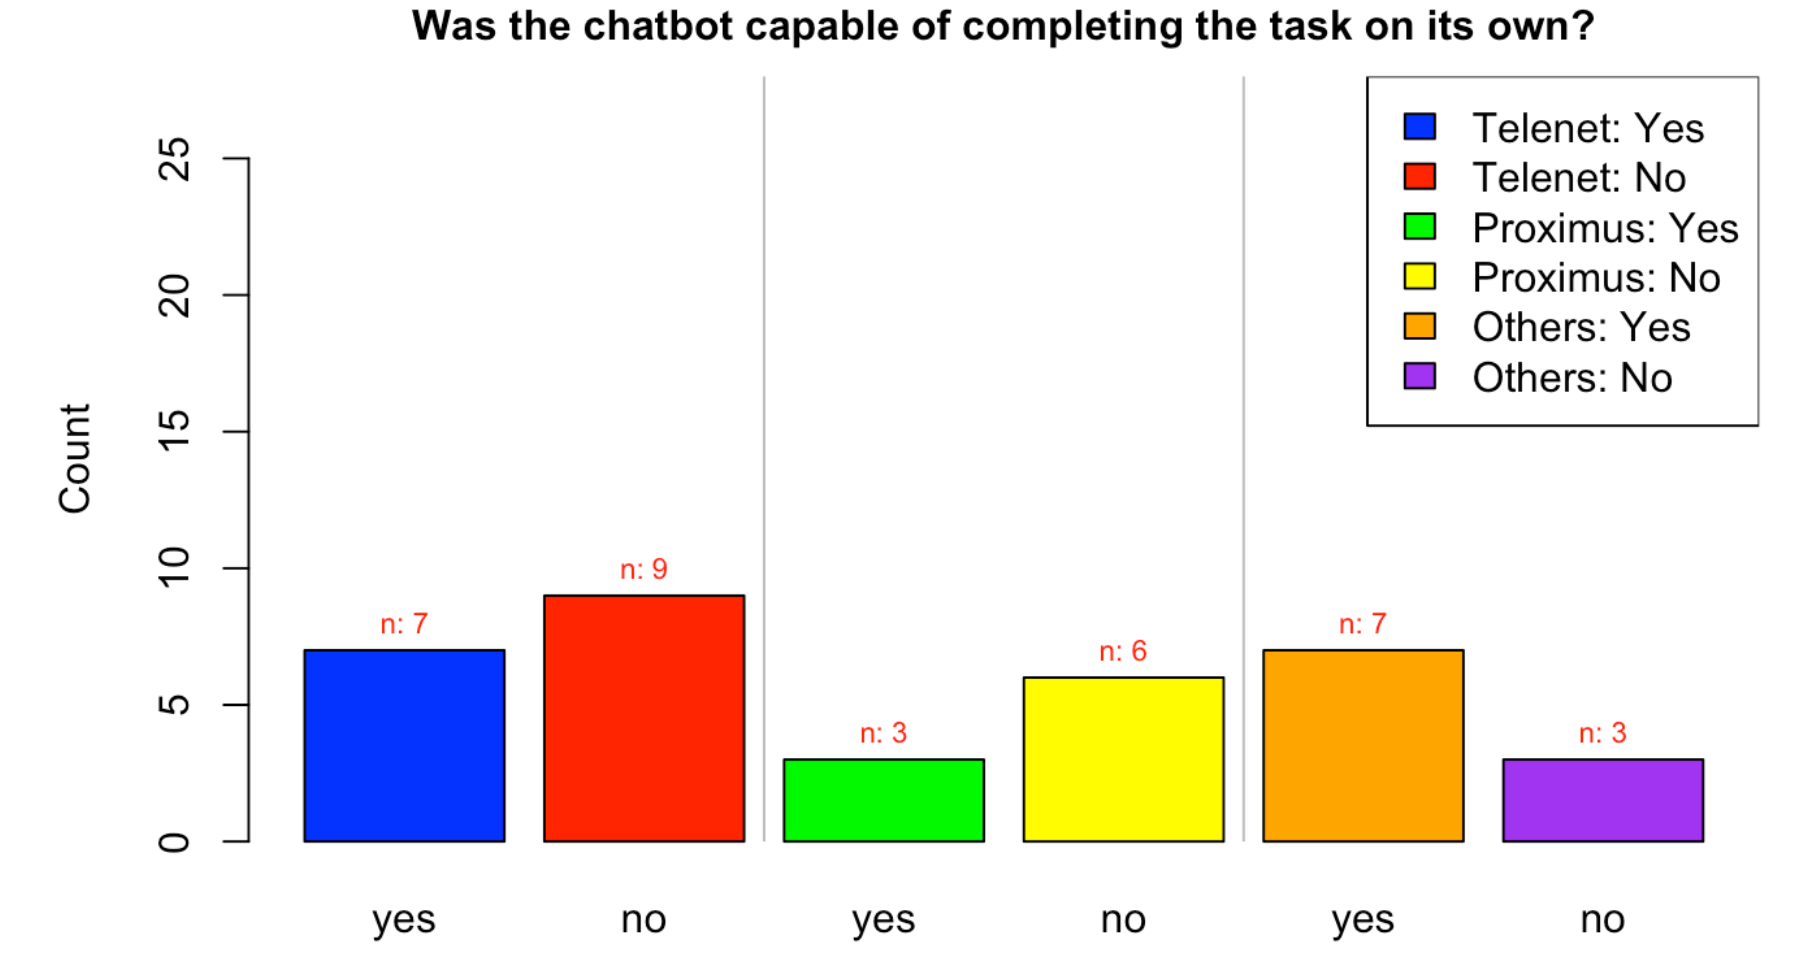
\includegraphics[width=\linewidth, scale=0.5]{../LaTeX/Figures/Comparative/DQ1b.png}s
	\caption{Responses about the dysfunctional question for \acrshort{qa} 1, question 2.}\label{fig:DQ1b}
\end{figure}
\break
A third question to gauge the capabilities of the chatbot to execute the requested task was about the expectations of the chatbot and if it lived up to them. The results show that the chatbot mostly lived up to expectations, even though it could not solve the task it was given.\\
\begin{figure}[!htb]
	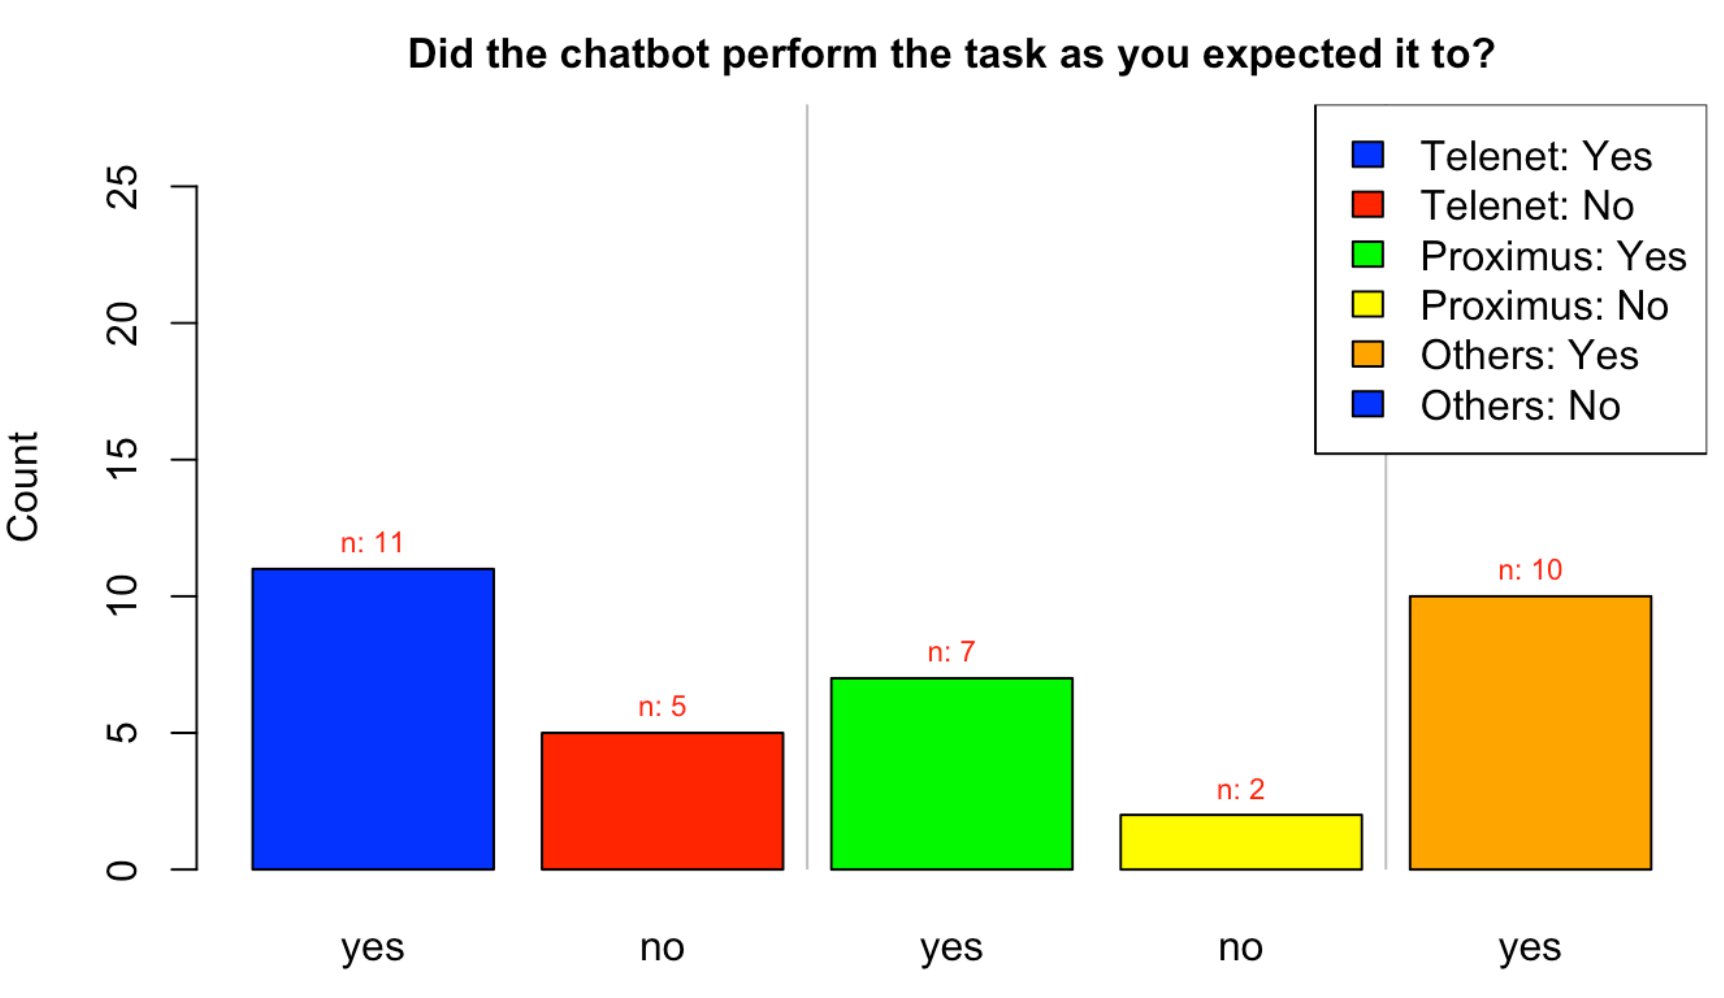
\includegraphics[width=\linewidth, scale=0.5]{../LaTeX/Figures/Comparative/Q1c.png}
	\caption{Responses about the functional question for \acrshort{qa} 1, question 3.}\label{fig:Q1c}
\end{figure}
A fourth and final question asked if the user could solve the problem after interacting with the chatbot. For Proximus, there was some pushback but for Telenet and the others, the majority voted yes.\\
\begin{figure}[!htb]
	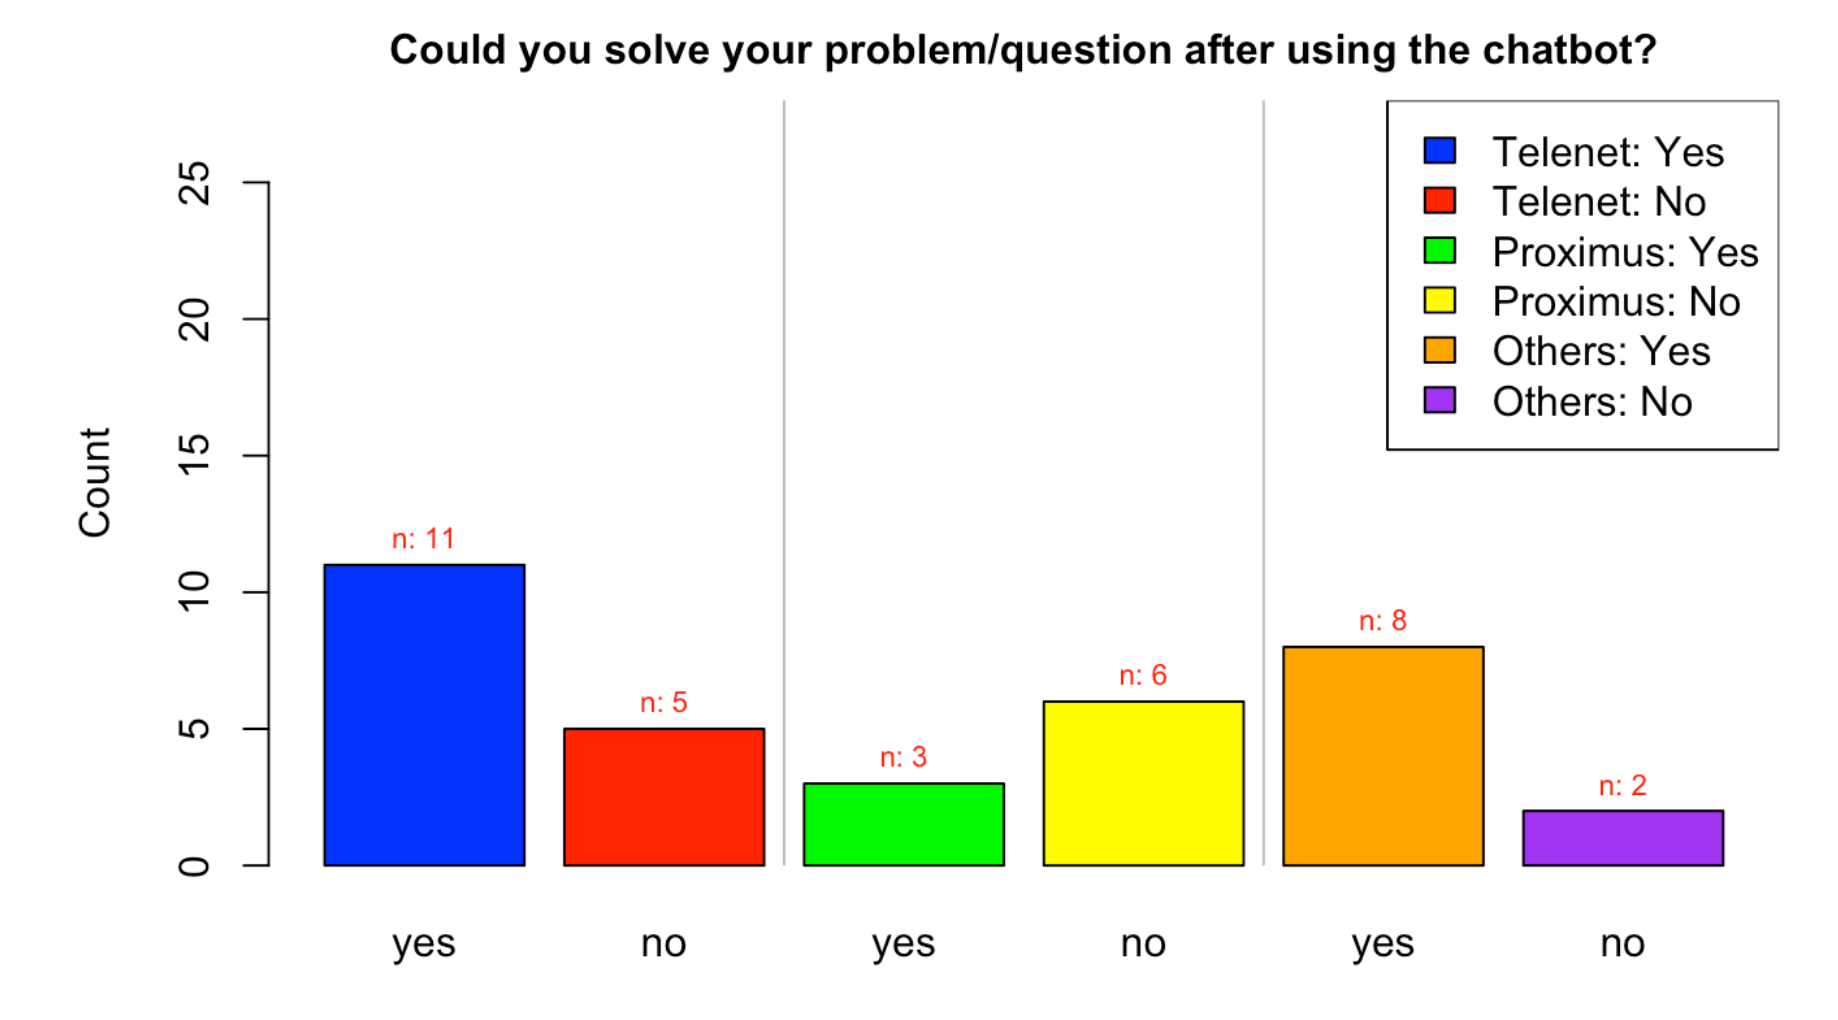
\includegraphics[width=\linewidth, scale=0.5]{../LaTeX/Figures/Comparative/DQ1c.png}
	\caption{Responses about the dysfunctional question for \acrshort{qa} 1, question 4.}\label{fig:DQ1c}
\end{figure}
\break
\ul{Attribute 2: Number of services}\\
\break
Attribute 2 looked at the services available and delivered by the chatbot in comparison to a human agent. The responses about whether a chatbot delivers a better service than a human agent were for both Telenet and the others an outstanding no whereas for Proximus, the votes were more divided, almost a 50-50 split.\\
\begin{figure}[!htb]
	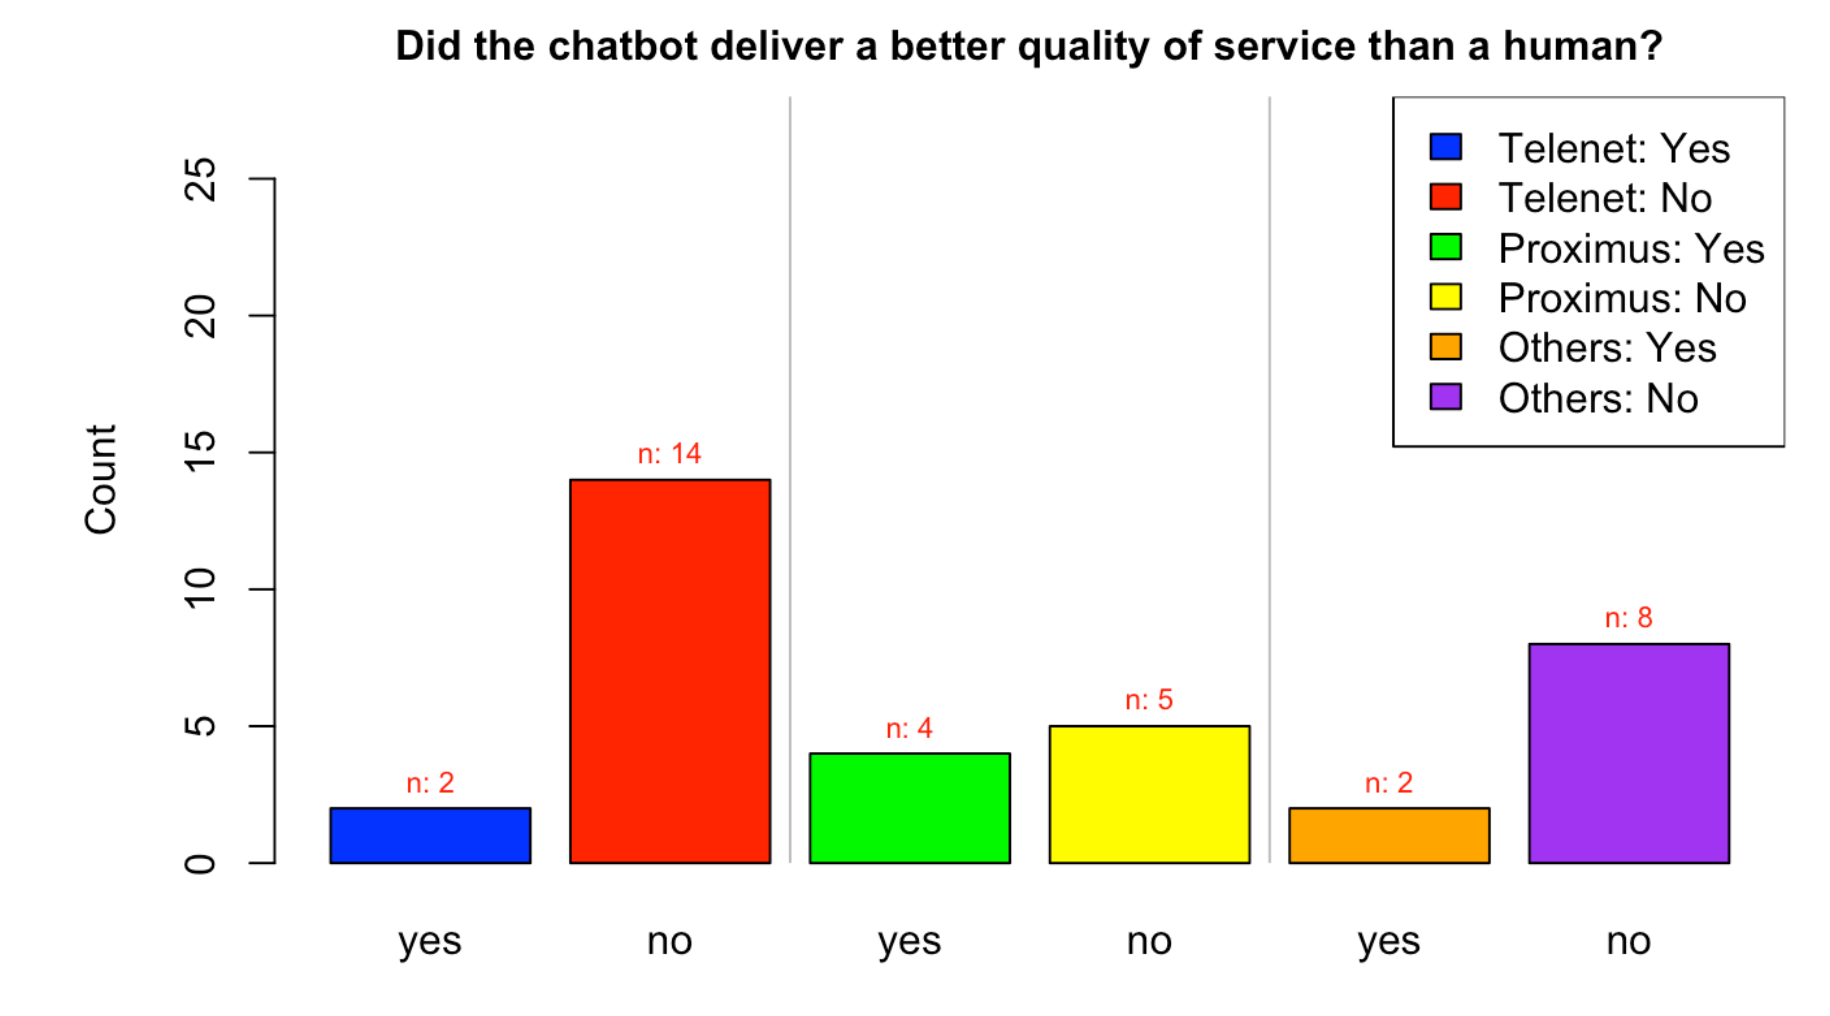
\includegraphics[width=\linewidth, scale=0.5]{../LaTeX/Figures/Comparative/Q2.png}
	\caption{Responses about the functional question for \acrshort{qa} 2.}\label{fig:Q2}
\end{figure}
When asked whether the service delivered by a human was of better quality, the responses for each group were almost always yes.\\
\begin{figure}[!htb]
	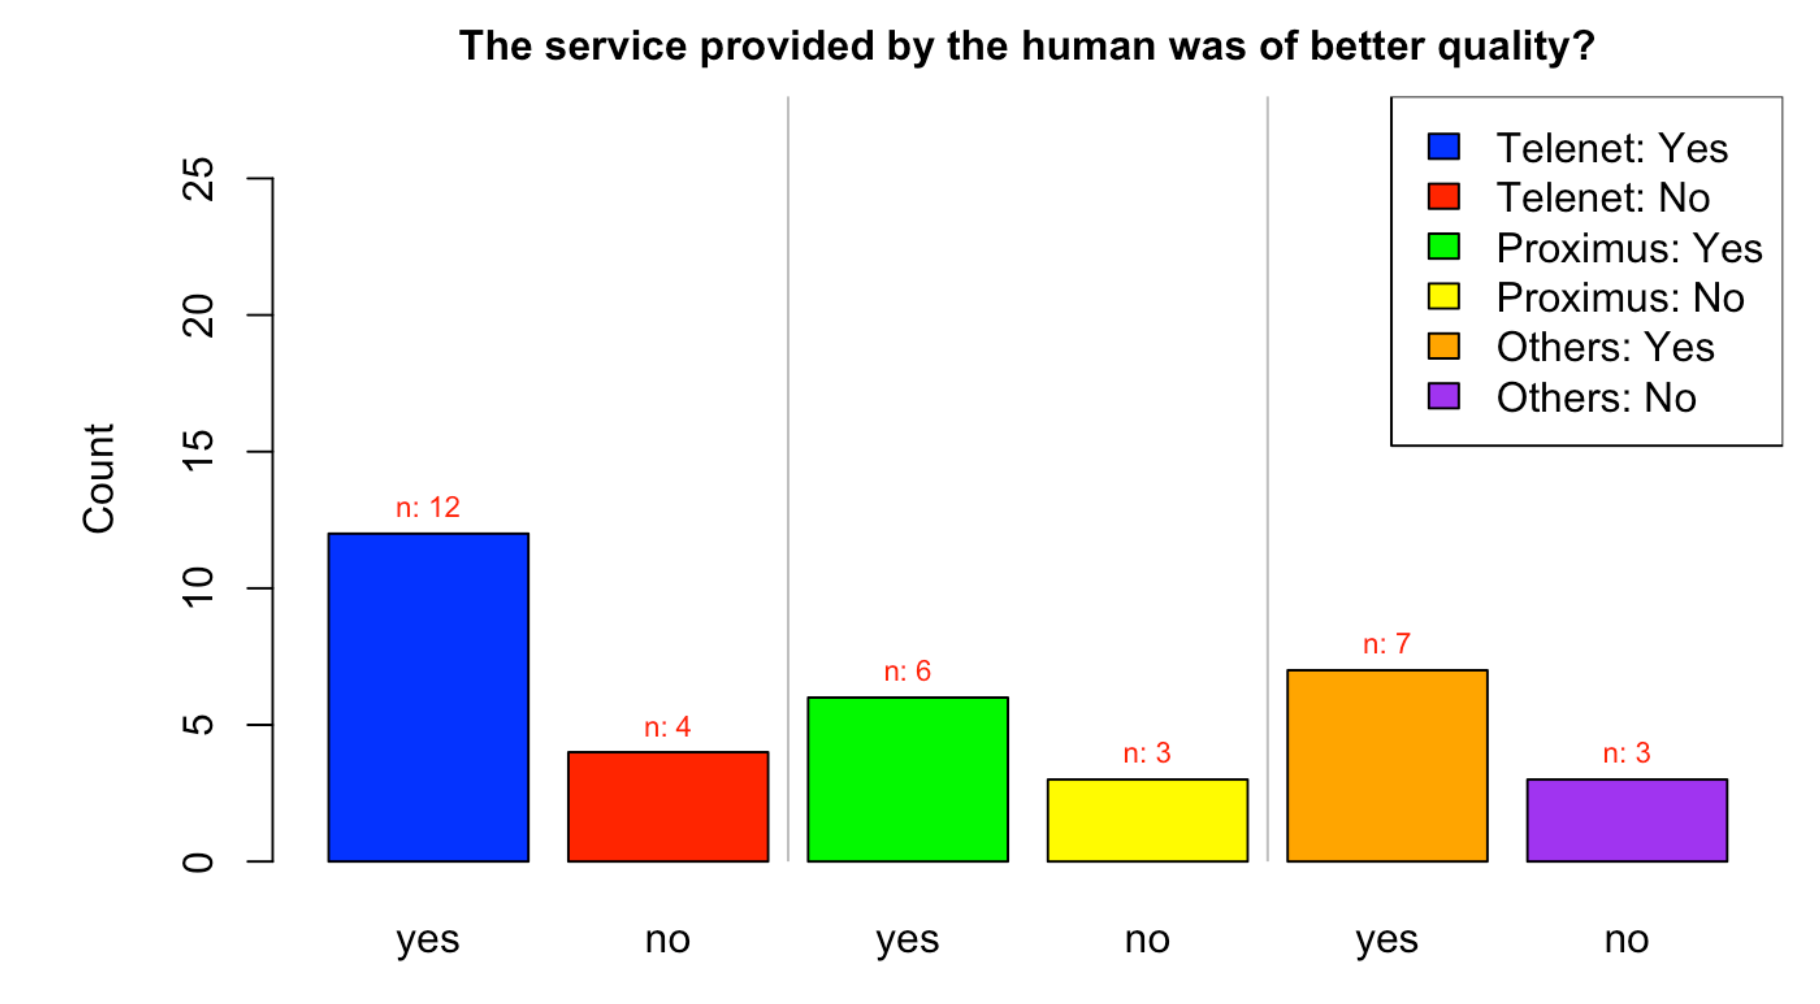
\includegraphics[width=\linewidth, scale=0.5]{../LaTeX/Figures/Comparative/DQ2.png}
	\caption{Responses about the dysfunctional question for \acrshort{qa} 2.}\label{fig:DQ2}
\end{figure}
\break
\ul{Attribute 3: Breadth of knowledge}\\
\break
When presented with the question "Did the chatbot contain enough knowledge to help with your problem", the responses for each group differ a lot. For Telenet, there is a 50-50 split. Proximus on the other hand is mostly negative. This contrasts the other group where the responses were mainly positive.\\
\begin{figure}[!htb]
	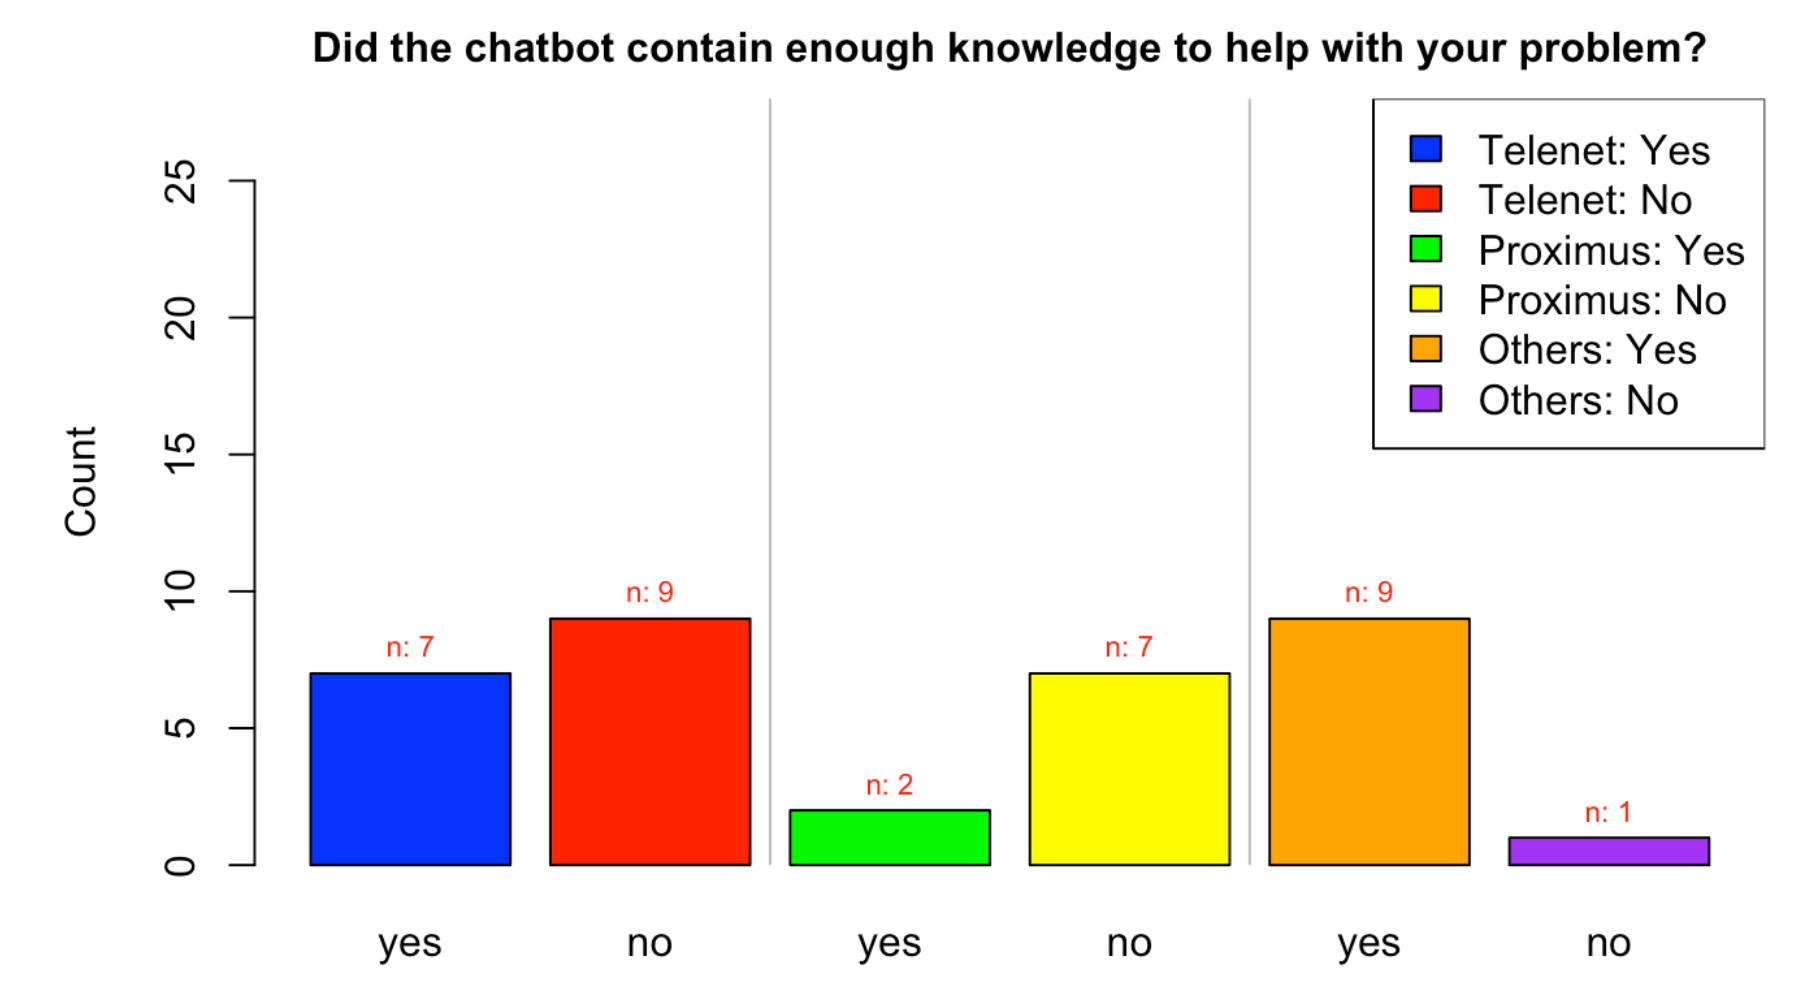
\includegraphics[width=\linewidth, scale=0.5]{../LaTeX/Figures/Comparative/Q3.png}
	\caption{Responses about the functional question for \acrshort{qa} 3, question 1.}\label{fig:Q3}
\end{figure}
When asking the inverse, the answers provided were more streamlined to be mostly negative. In other words, the chatbot knows what he is talking about.\\
\begin{figure}[!htb]
	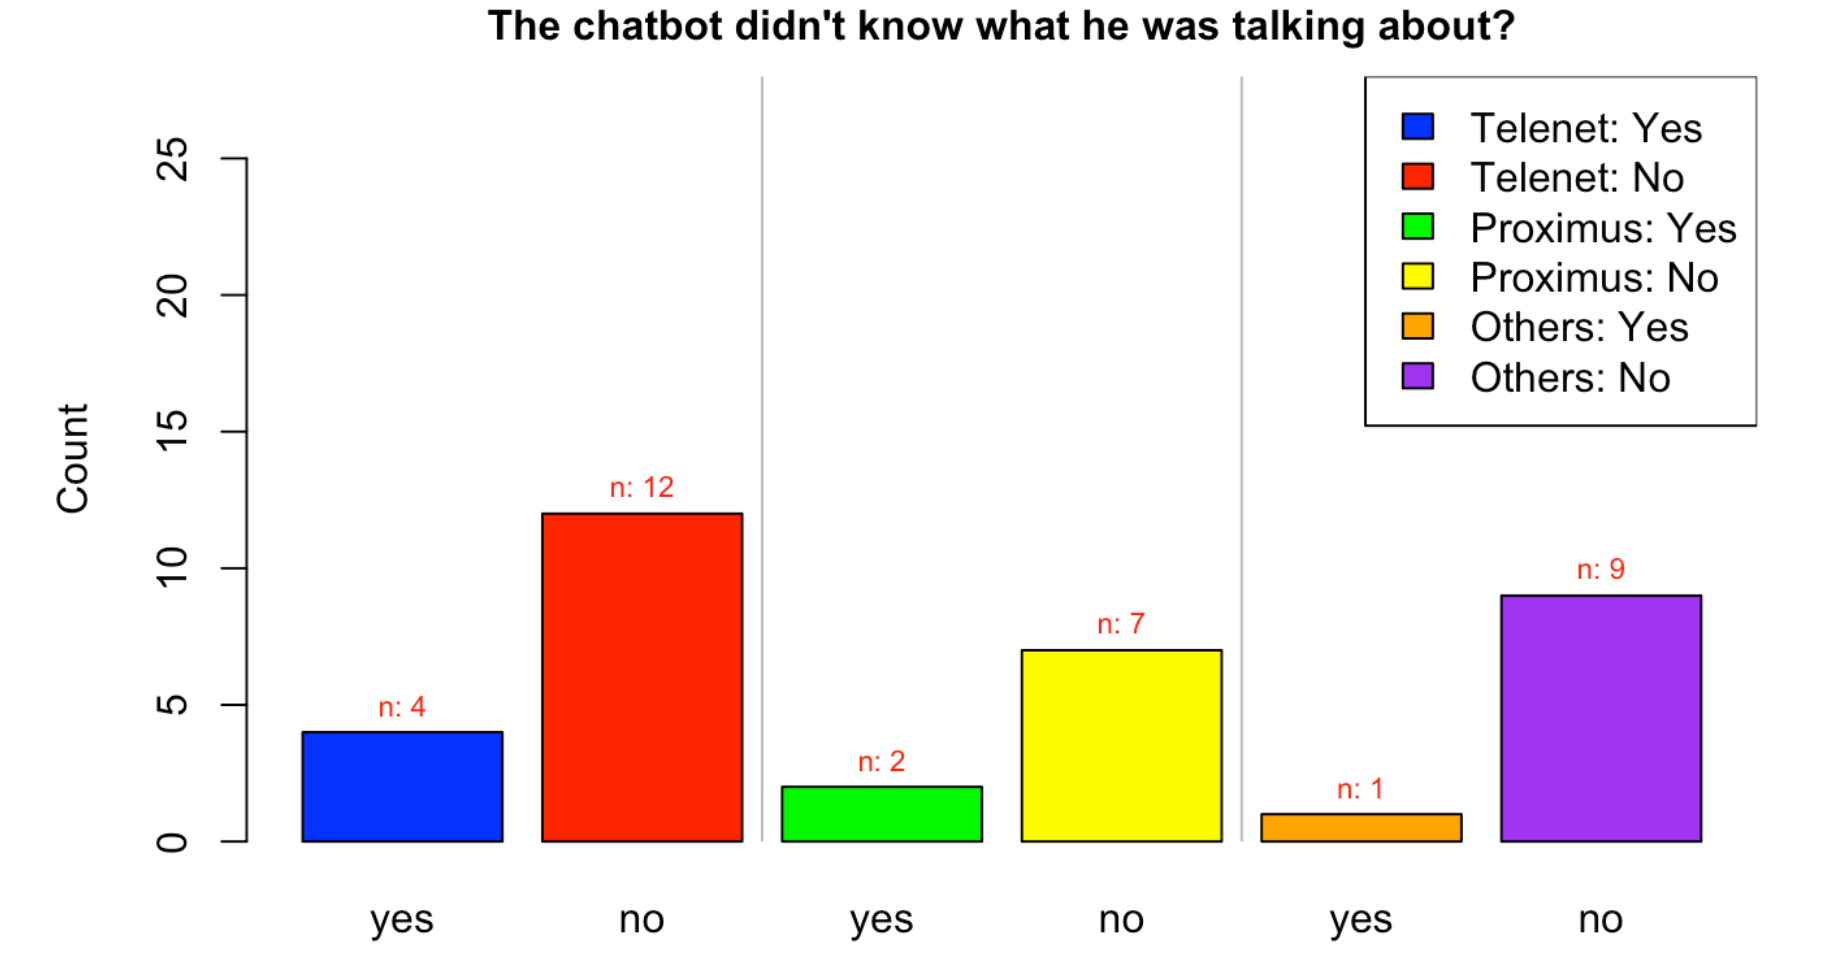
\includegraphics[width=\linewidth, scale=0.5]{../LaTeX/Figures/Comparative/DQ3.png}
	\caption{Responses about the dysfunctional question for \acrshort{qa} 3, question 1.}\label{fig:DQ3}
\end{figure}
\break
The second question checks if the chatbot asked relevant questions to gather extra information about the problem. It measures if the chatbot can gather more information if the given context isn't clear enough. Telenet and the others were mostly positive, Proximus has a 50-50 split.\\
\begin{figure}[!htb]
	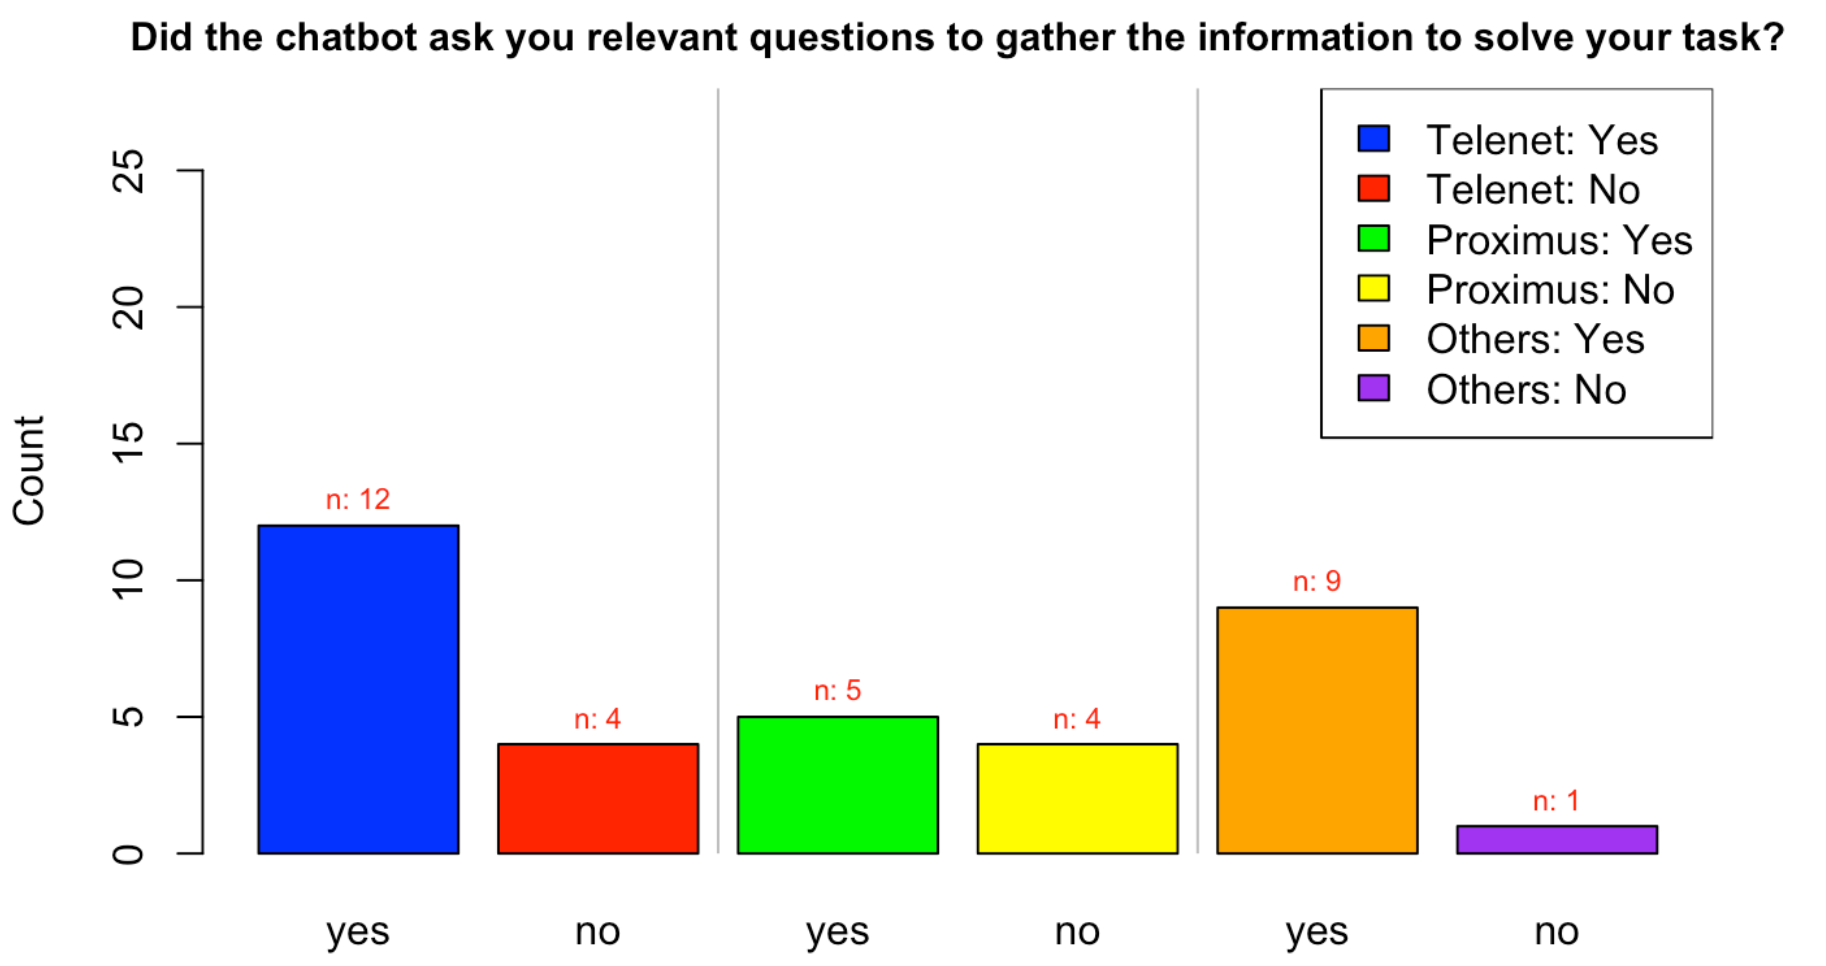
\includegraphics[width=\linewidth, scale=0.5]{../LaTeX/Figures/Comparative/Q3b.png}
	\caption{Responses about the functional question for \acrshort{qa} 3, question 2.}\label{fig:Q3b}
\end{figure}
When looking at the reverse, Telenet seemed to not ask the right questions whereas Proximus and the others were about evenly split.\\
\begin{figure}[!htb]
	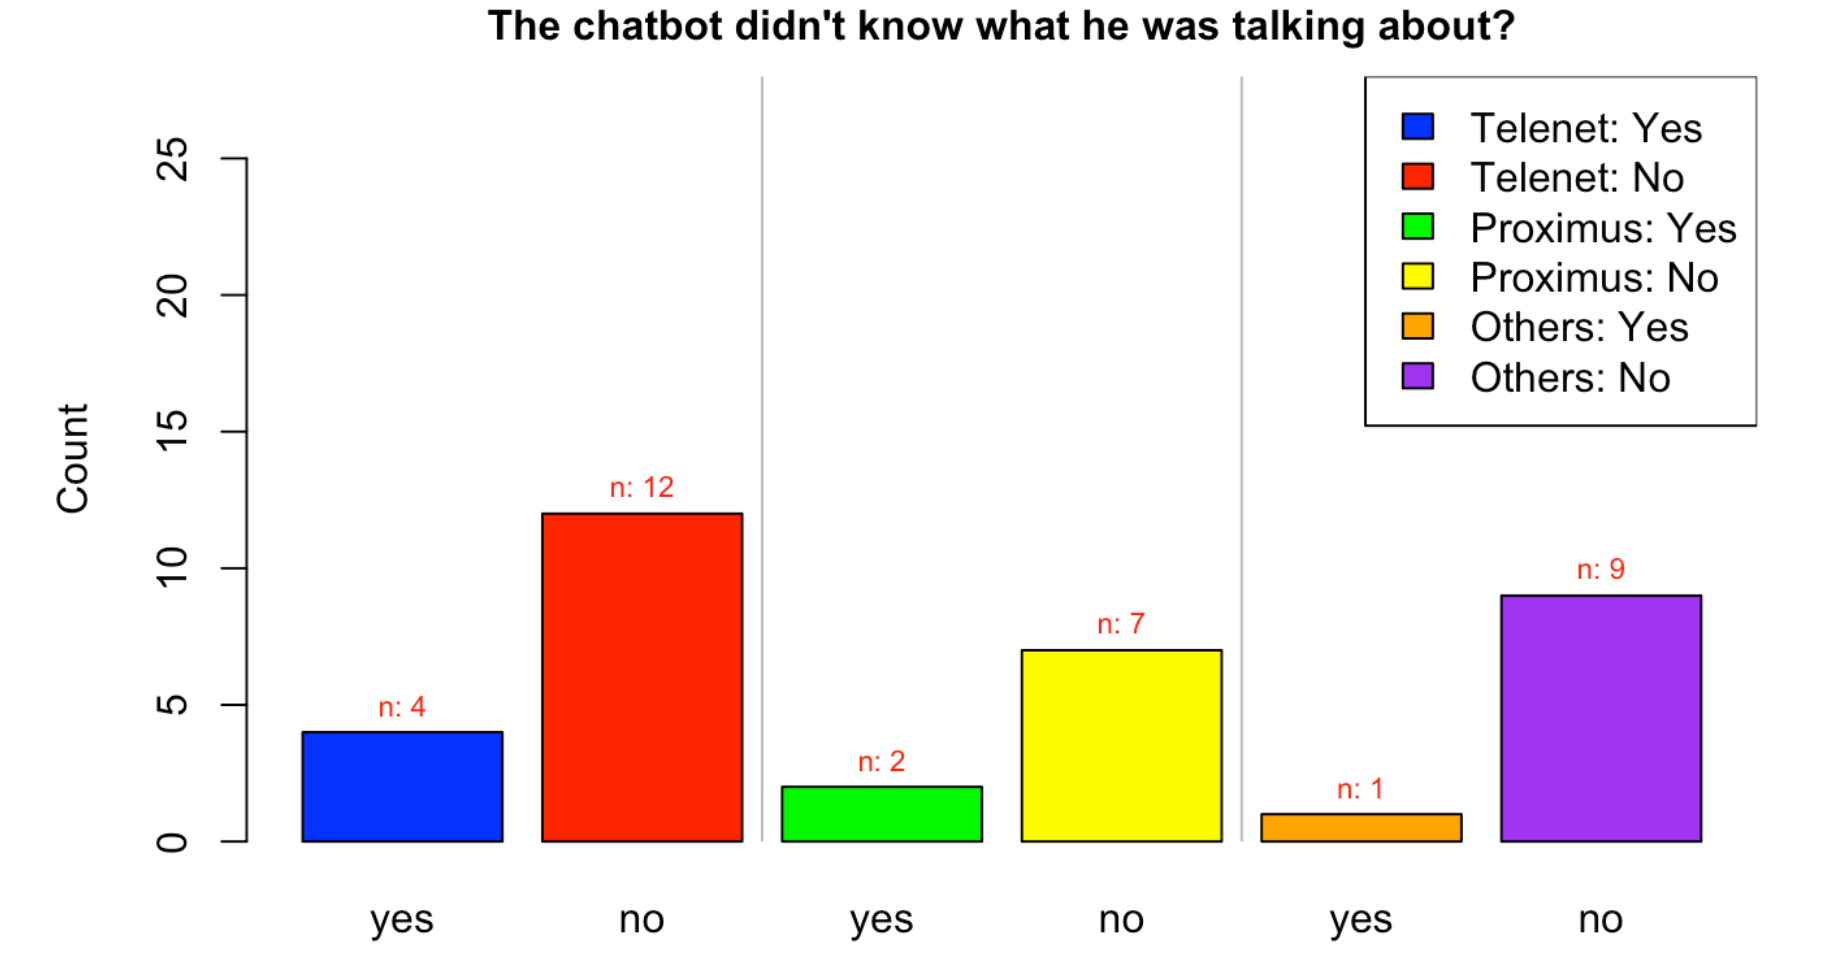
\includegraphics[width=\linewidth, scale=0.5]{../LaTeX/Figures/Comparative/DQ3.png}
	\caption{Responses about the dysfunctional question for \acrshort{qa} 3, question 2.}\label{fig:DQ3}
\end{figure}
\break 
\ul{Attribute 4: Ease of use}\\
\break
There weren't any complications when using any of the chatbots.
\begin{figure}[!htb]
	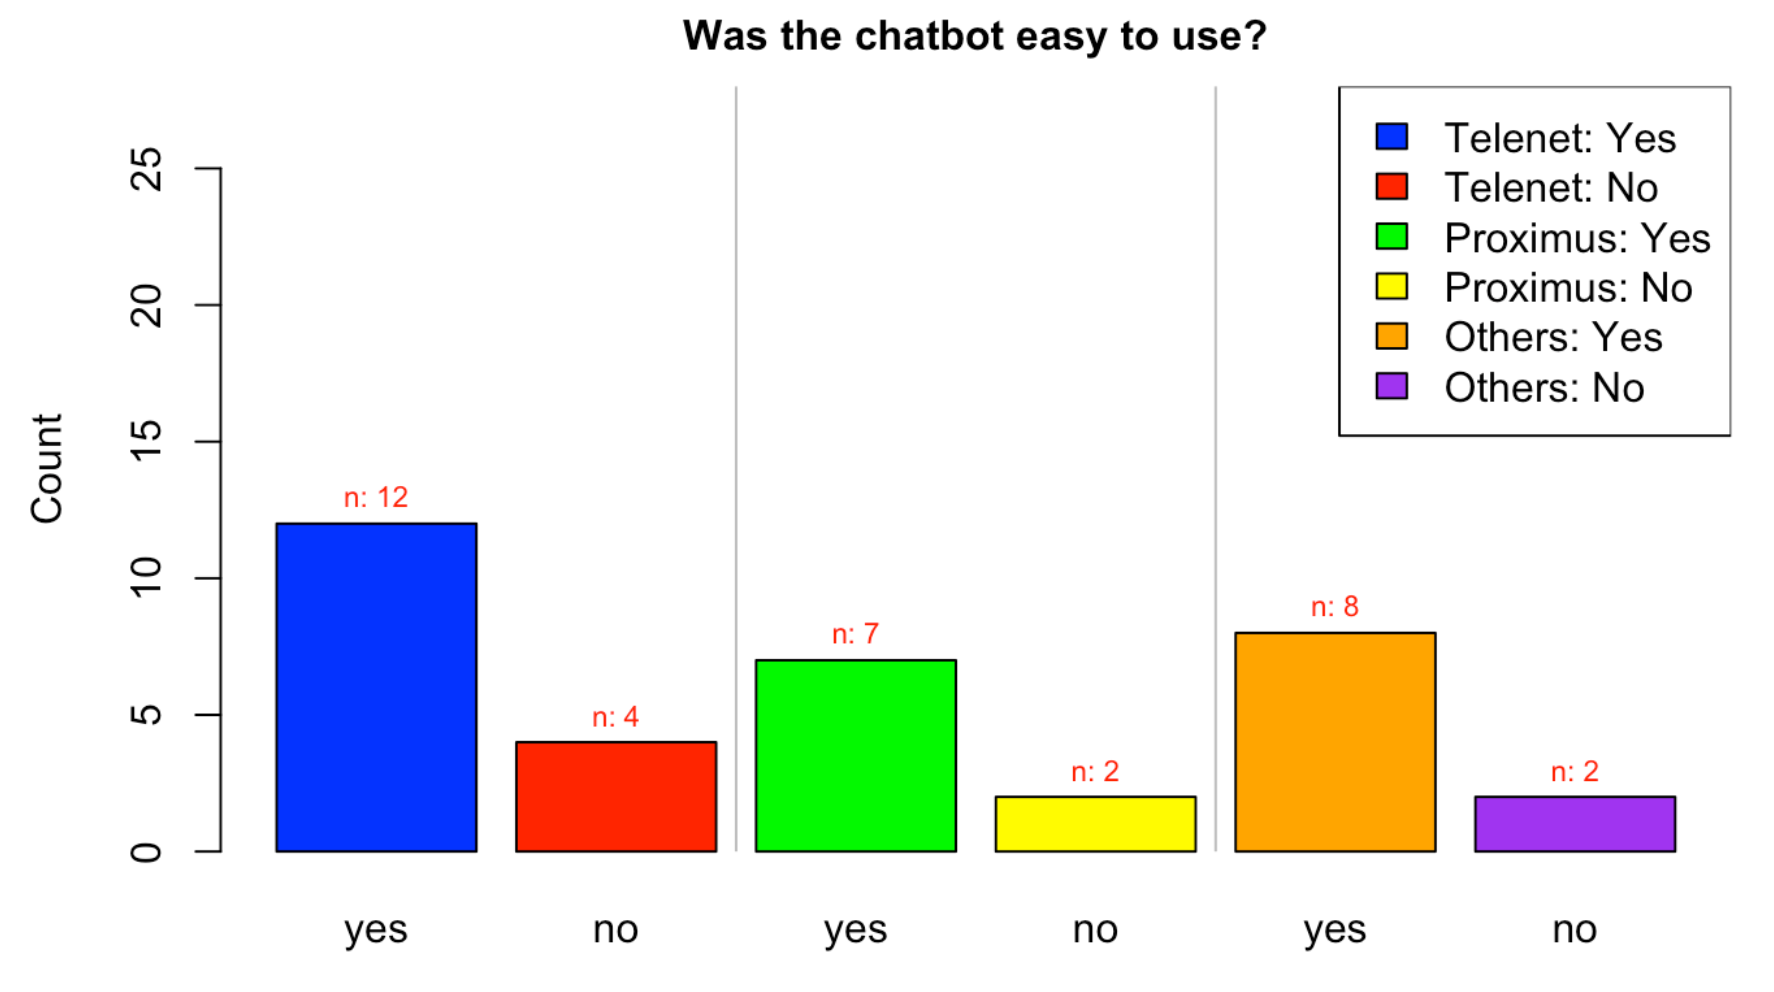
\includegraphics[width=\linewidth, scale=0.5]{../LaTeX/Figures/Comparative/Q4.png}
	\caption{Responses about the functional question for \acrshort{qa} 4.}\label{fig:Q4}
\end{figure}
Looking at the dysfunctional version of this question, the values confirm what has been seen for Telenet and the others but dispute the result for Proximus. There seem to be some problems when using the Proximus chatbot.\\
\begin{figure}[!htb]
	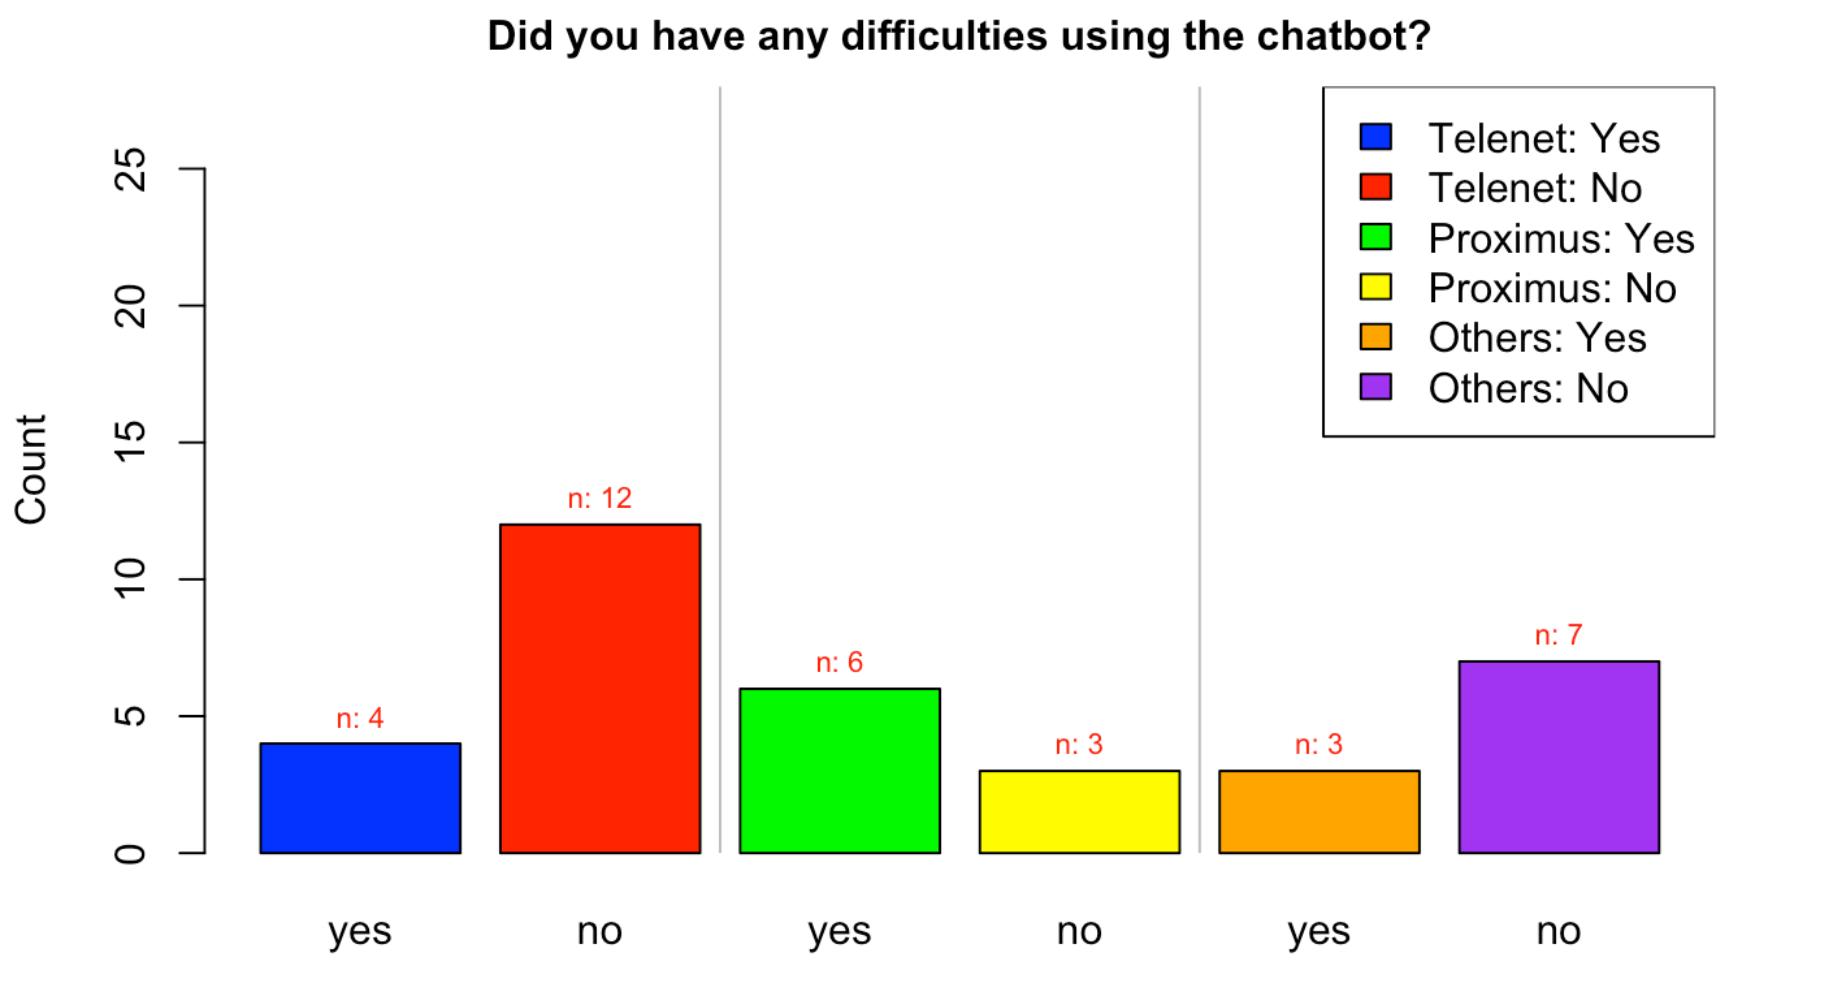
\includegraphics[width=\linewidth, scale=0.5]{../LaTeX/Figures/Comparative/DQ4.png}
	\caption{Responses about the dysfunctional question for \acrshort{qa} 4.}\label{fig:DQ4}
\end{figure}
\break
\ul{Attribute 5: Enjoyable interaction}\\
\break
The 5\textsuperscript{th} attribute takes into consideration the interaction a user has with the chatbot. The first question asked if the chatbot was polite. The data shows that every group generally has a polite chatbot.\\
\begin{figure}[!htb]
	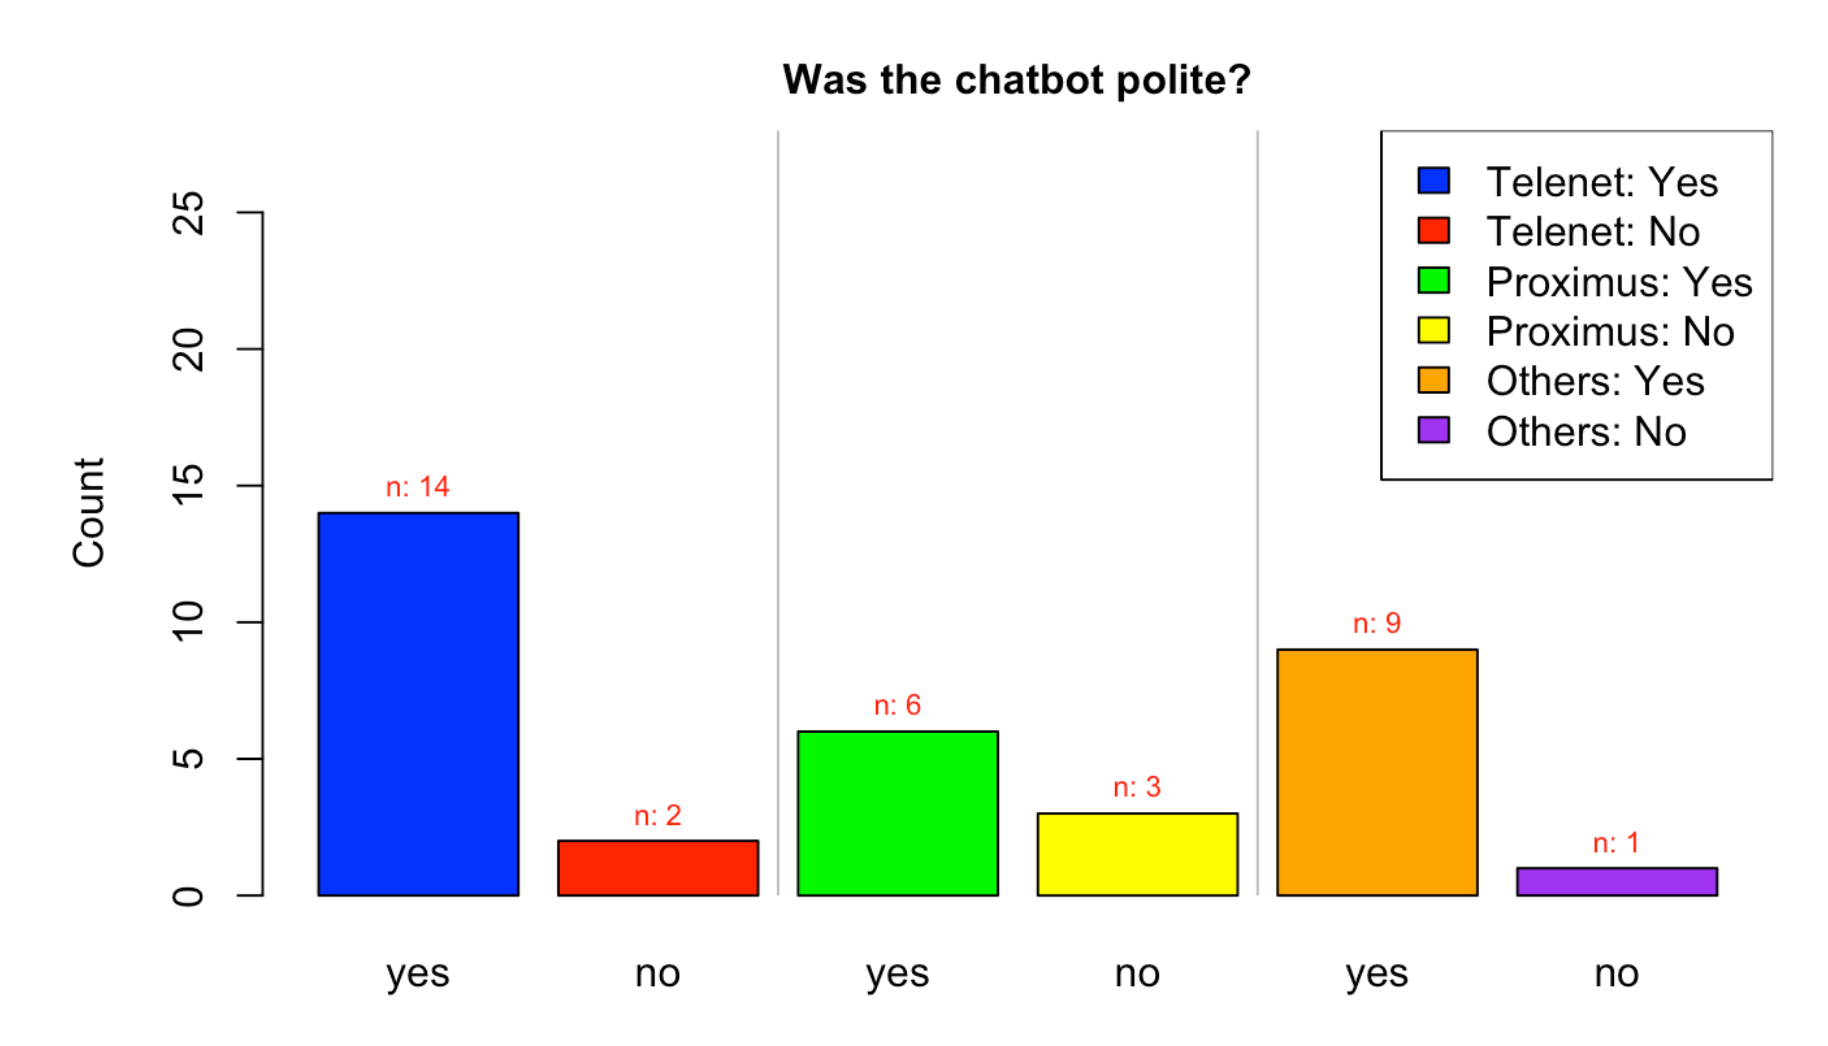
\includegraphics[width=\linewidth, scale=0.5]{../LaTeX/Figures/Comparative/Q5.png}
	\caption{Responses about the functional question for \acrshort{qa} 5, question 1.}\label{fig:Q5}
\end{figure}
\break
When asked if the chatbot interacted in a respectful way, the answers for Telenet were mostly positive, Proximus is once again divided around the 50\% mark and the others scored 100\%.\\
\begin{figure}[!htb]
	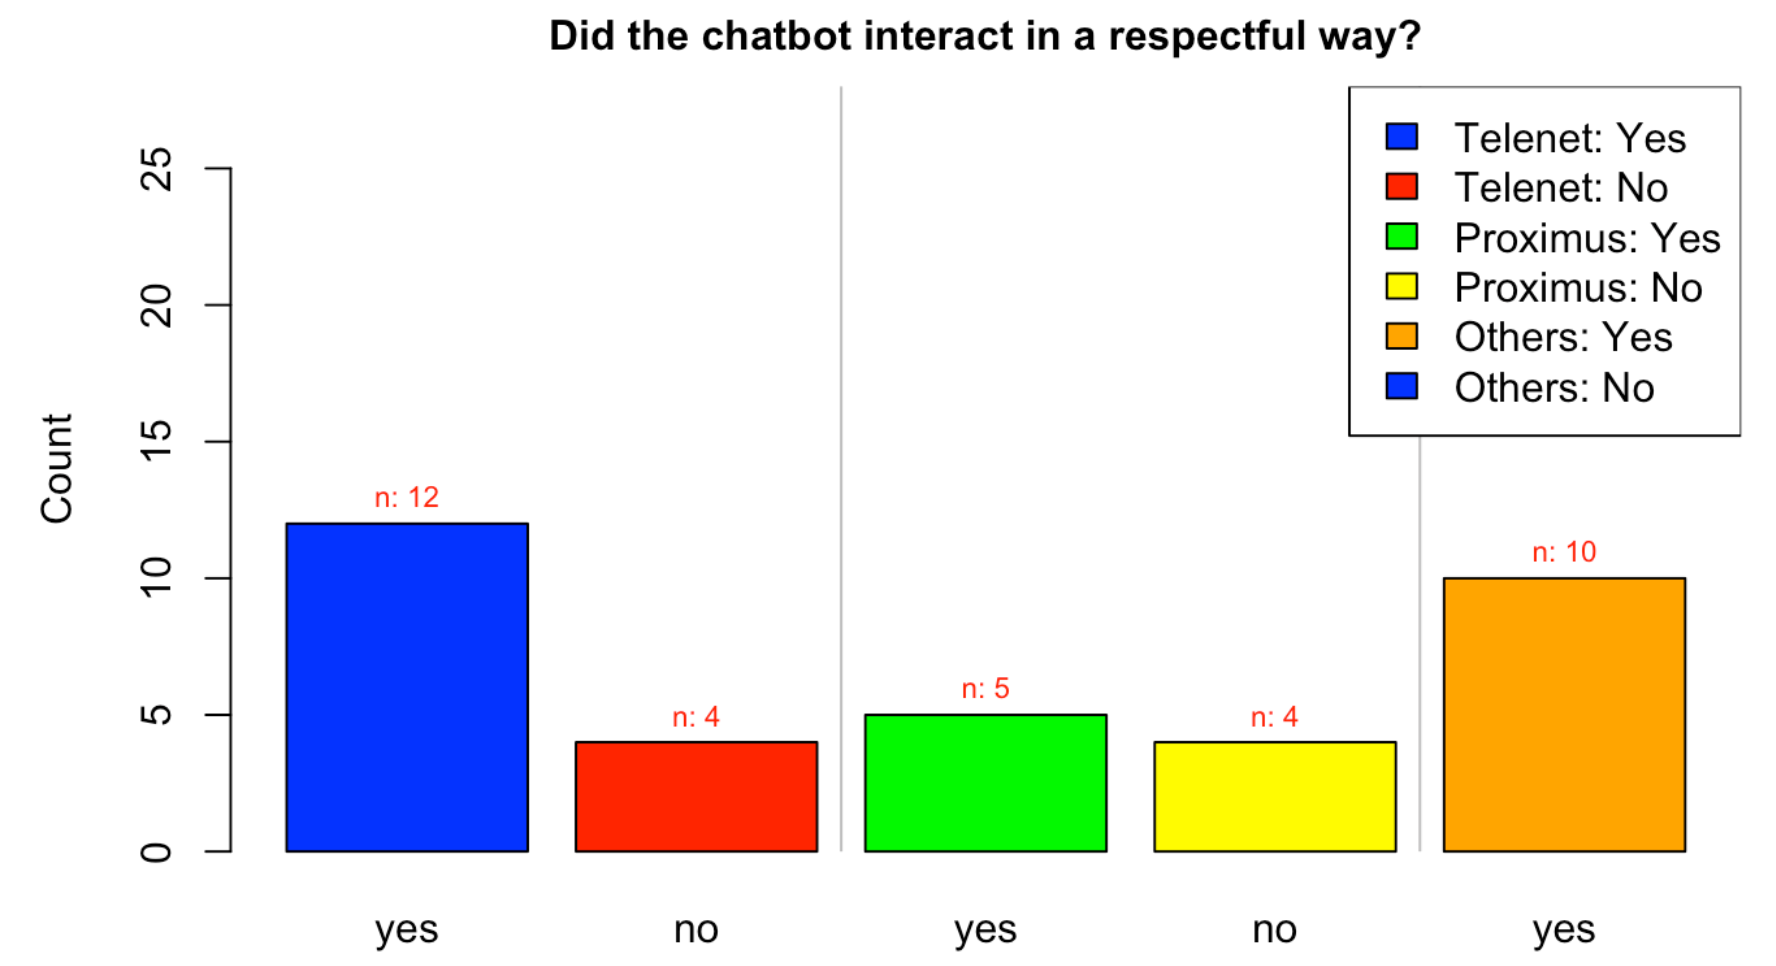
\includegraphics[width=\linewidth, scale=0.5]{../LaTeX/Figures/Comparative/DQ5.png}
	\caption{Responses about the dysfunctional question for \acrshort{qa} 5, question 1.}\label{fig:DQ5}
\end{figure}
\break
The second question asks if the user liked interacting with the chatbot. Telenet is evenly split and both Proximus and the others are mostly positive.\\
\begin{figure}[!htb]
	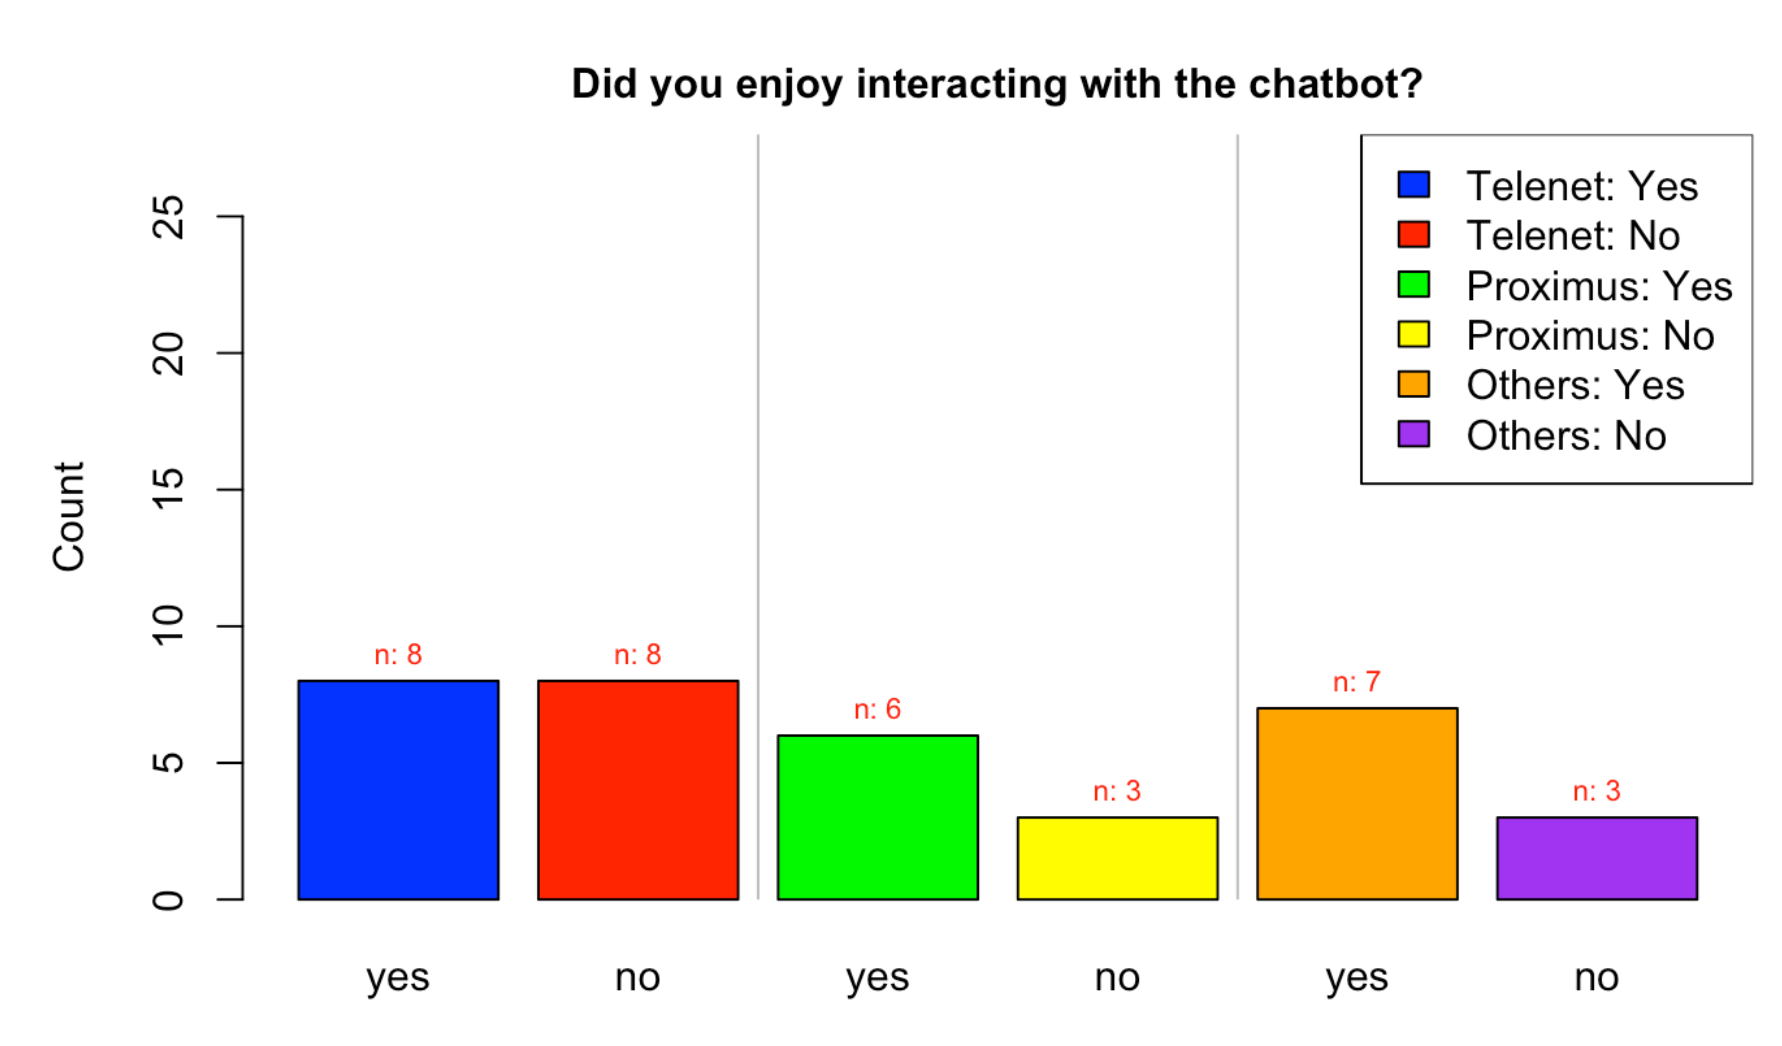
\includegraphics[width=\linewidth, scale=0.5]{../LaTeX/Figures/Comparative/Q5b.png}
	\caption{Responses about the functional question for \acrshort{qa} 5, question 2.}\label{fig:Q5b}
\end{figure}
When asked the reverse, both Telenet and the others are divided evenly. Proximus has more negative than positive responses meaning, it wasn't a task to interact with their chatbot.\\
\begin{figure}[!htb]
	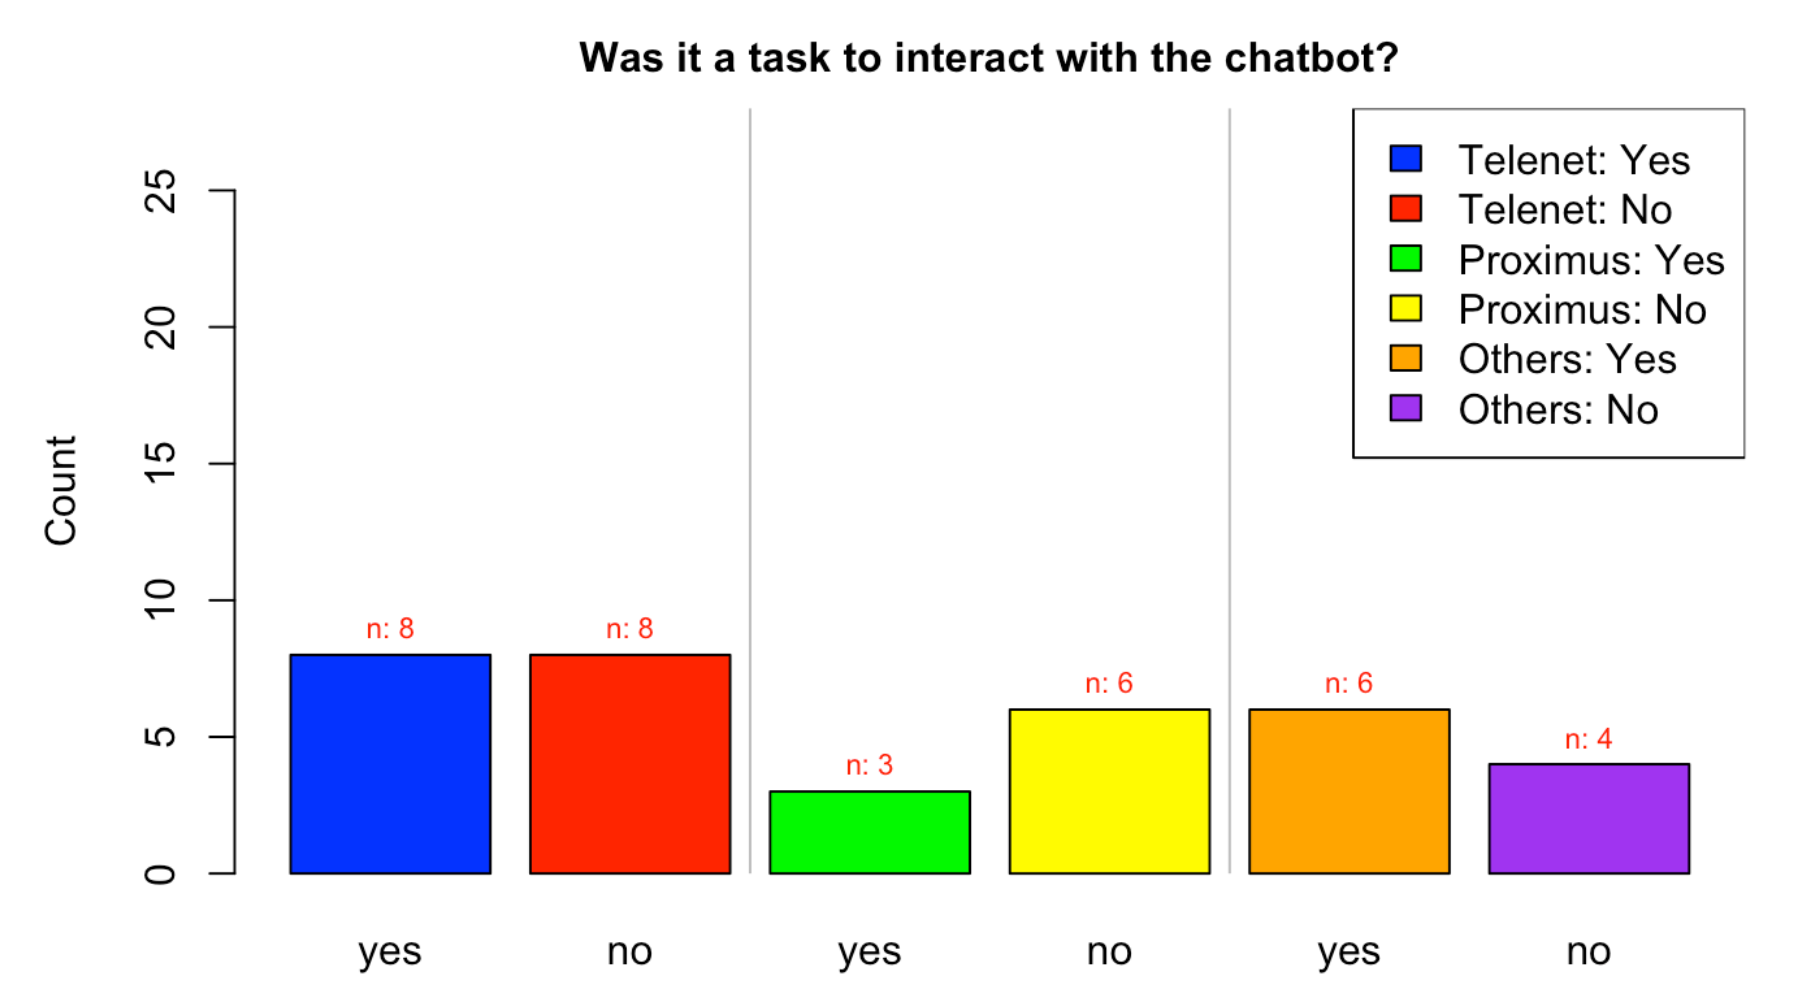
\includegraphics[width=\linewidth, scale=0.5]{../LaTeX/Figures/Comparative/DQ5b.png}
	\caption{Responses about the dysfunctional question for \acrshort{qa} 5, question 2.}\label{fig:DQ5b}
\end{figure}
\FloatBarrier
\subsection{Importance Study - Kano}
\subsubsection{Discrete analysis}
To start with the KANO analysis, there first had to be made a clear mapping between the functional and dysfunctional question and which label of KANO would be assigned to the outcome of this mapping (see Figure \ref{fig:kanoOverview}).
\begin{figure}[htb!]
	\centering
	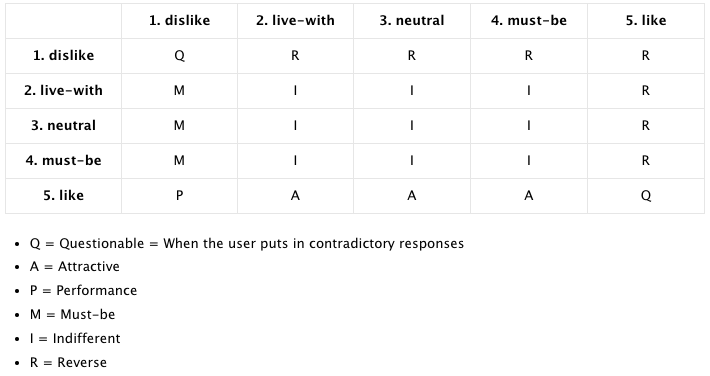
\includegraphics[width=\linewidth]{../LaTeX/Figures/Kano/KANOOverview.png}
	\caption{The mapping between the functional and dysfunctional question and the KANO label associated.}
	\label{fig:kanoOverview}
\end{figure}
\break
Afterwards, for each scenario (section 3.3.3) as well as the general questions of the survey, the answers were counted and added per label. The highest label was assigned. If there was an overlap between two or more labels, the label with the most impact was chosen (see 3.3.2 - Data Evaluation Method).\\
An overview of the label assigned to each entry can be found in Figure \ref{fig:kanoTable}. S1, S2 and S3 refer to the 3 different scenarios.
\begin{figure}[!htb]
	\centering
	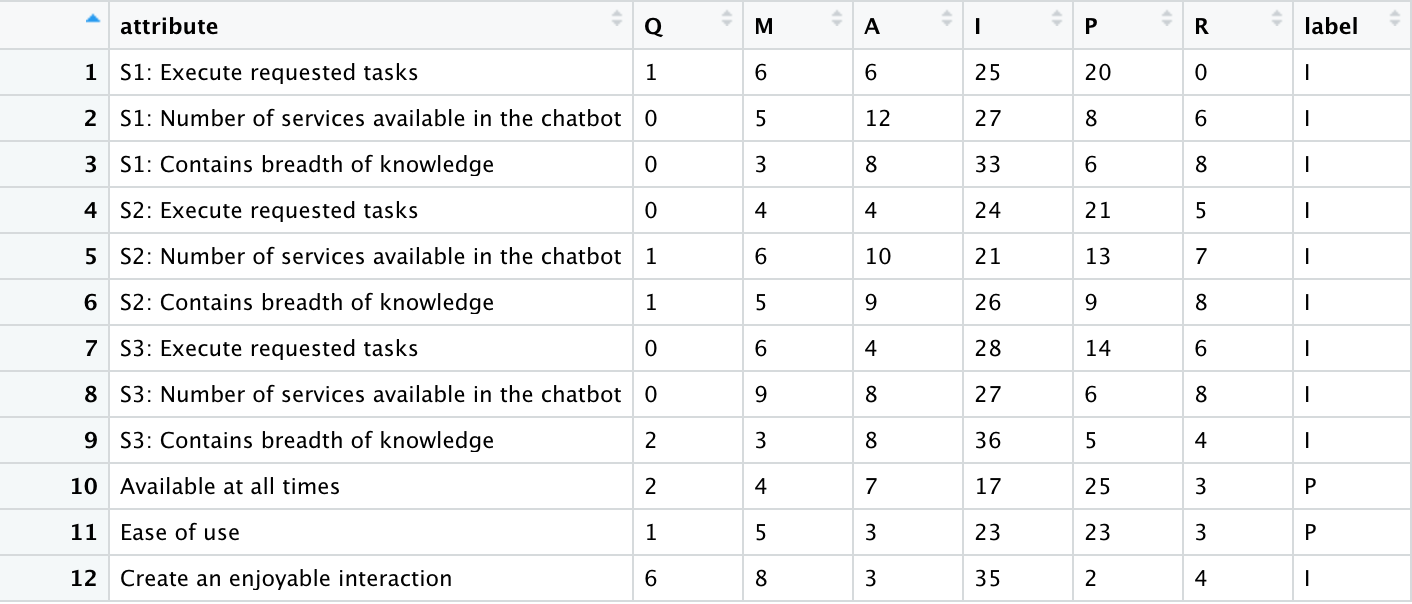
\includegraphics[width=\linewidth]{../LaTeX/Figures/Kano/KanoTable.png}
	\caption{Each entry with it's assigned KANO label.}
	\label{fig:kanoTable}
\end{figure}
\subsubsection{Continuous analysis}
Now, each entry has a label assigned to it and for every entry, the different categories are counted. Based on this, both the satisfaction as well as the dissatisfaction coefficient can be calculated. The calculations can be seen in Figure \ref{fig:satisfactionCoef} and Figure \ref{fig:dissatisfactionCoef}.
\begin{figure}[!htb]
	\centering
	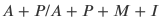
\includegraphics{../LaTeX/Figures/Kano/SatisfactionCoef.png}
	\caption{The satisfaction coefficient.}
	\label{fig:satisfactionCoef}
\end{figure}
\begin{figure}[!htb]
	\centering
	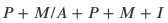
\includegraphics{../LaTeX/Figures/Kano/DissatisfactionCoef.png}
	\caption{The dissatisfaction coefficient.}
	\label{fig:dissatisfactionCoef}
\end{figure}
\break
After calculating both these scores for each entry, they were plotted in  a scatter plot, dividing them up into one of the four main categories of KANO. The categorisation can be found in Figure \ref{fig:satisfactionPlot}
\begin{figure}[!htb]
	\centering
	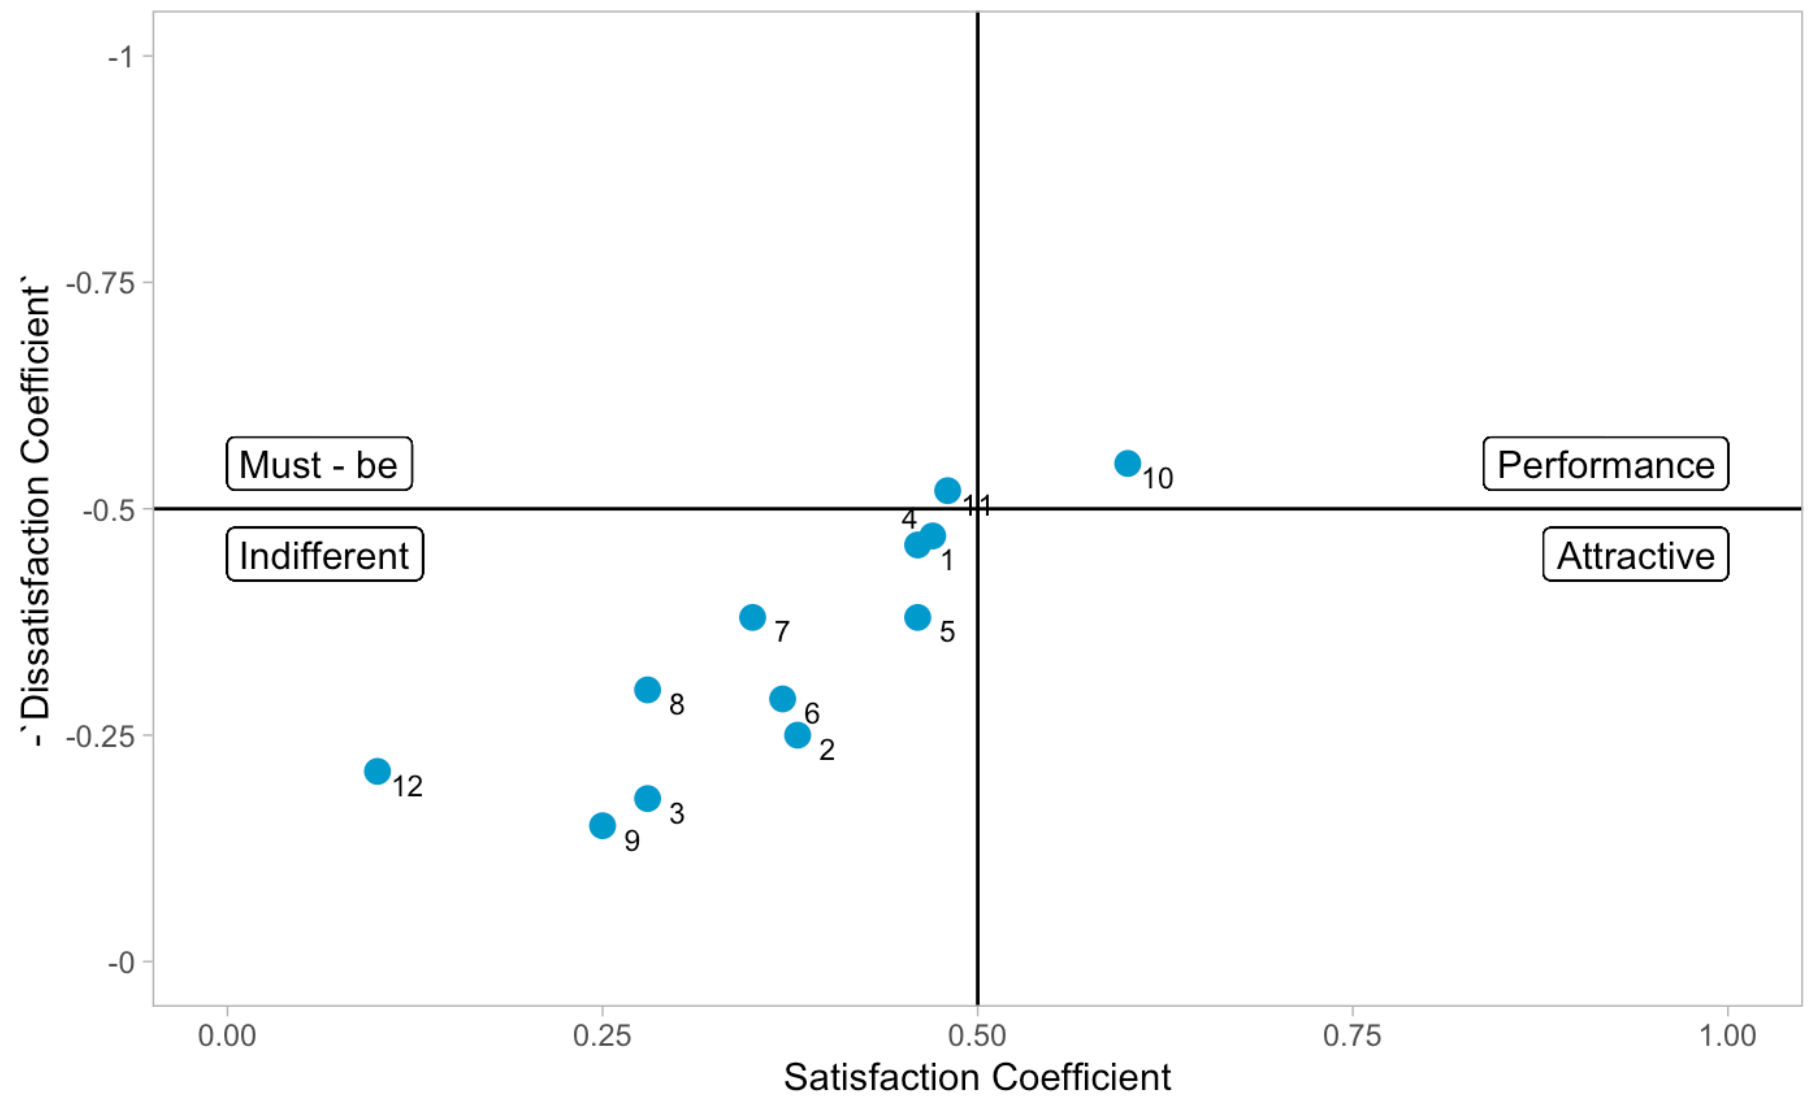
\includegraphics[width=\linewidth]{../LaTeX/Figures/Kano/SatisfactionPlot.png}
	\caption{The satisfaction/dissatisfaction plot.}
	\label{fig:satisfactionPlot}
\end{figure}

\begin{longtable}{|c|l|}
	\hline
	\textbf{Item} & \multicolumn{1}{c|}{\textbf{Attribute}}         \\ \hline
	\endfirsthead
	\endhead
	\textbf{1}    & S1: Execute requested tasks                     \\ \hline
	\textbf{2}    & S1: Number of services available in the chatbot \\ \hline
	\textbf{3}    & S1: Contains breadth of knowledge               \\ \hline
	\textbf{4}    & S2: Execute requested tasks                     \\ \hline
	\textbf{5}    & S2: Number of services available in the chatbot \\ \hline
	\textbf{6}    & S2: Contains breadth of knowledge               \\ \hline
	\textbf{7}    & S3: Execute requested tasks                     \\ \hline
	\textbf{8}    & S3: Number of services available in the chatbot \\ \hline
	\textbf{9}    & S3: Contains breadth of knowledge               \\ \hline
	\textbf{10}   & Available at all times                          \\ \hline
	\textbf{11}   & Ease of use                                     \\ \hline
	\textbf{12}   & Create an enjoyable interaction                 \\ \hline
	\caption{An Overview of the plotted entries in the satisfaction/dissatisfaction plot.}
	\label{tab:kanoSatisfactionDissatisfactionTable}
\end{longtable}

\section{Discussion}
\subsubsection{RQ1: Are current chatbots effective in helping people and
	solving their problems?}
\ul{H1: Current chatbots execute requested tasks correctly.}\\
At this point, there seems to be a split customer base about the delivered service by the chatbot. Some are happy with the execution of their task where others were not. They also indicate that the chatbot needs help from an agent but this seemed to match their expectations. In the end, most could solve their problem with the help of the chatbot.\\
\break
\ul{H2: Current chatbots can deliver the same services as a human
	agent.}\\
The data clearly shows that people do not think chatbots can deliver the same services as a human agent to the same quality.\\
\break
\ul{H3: Current chatbots contain enough knowledge to provide good
	assistance.}\\
There seems to be a big split between the customers. Depending on the provider, around 50\% think the chatbot is knowledgeable enough to help with their problem. When the chatbot did not have enough context to solve a question, depending on the situation, around 50\% think the chatbot did not ask the right questions to gather the needed information.\\
\break
\textbf{RQ1:} The opinions are divided. In some cases they are effective, in others they are not but they perform up to expectations from the customer.\\
\subsubsection{RQ2: Are current chatbots easy to use and accessible?}
\ul{H4: Current chatbots are easy to use.}\\
In general, there does not seem to be a problem when using the chatbot.\\
\break
\ul{H5: Current chatbots are available at all times (24/7).}\\
Each provider provides a chatbot that is available 24/7.\\
\break
\textbf{RQ2:} Yes, chatbots are easy to use and accessible.\\
\subsubsection{RQ3: Do current chatbots create a pleasant customer experience?}
\ul{H6: Current chatbots create an enjoyable interaction.}\\
Chatbots are generally perceived to be polite to interact with and most didn't mind interacting with a chatbot.\\
\break
\textbf{RQ3:} It is not yet perceived as enjoyable but it is not a task either.
\subsubsection{Main question}
The influence on the customer experience can be found in the ease of answering simple questions via the chatbot. On the other hand, more complex questions that cannot be solved might lead to frustrations.\\
For the business value, the influence is found in reducing costs for the help desk. The company is 24/7 available for support. The negative aspects force the providers to improve their chatbot with new technologies are more advanced \acrshort{ai} techniques.

\subsection{Quality attributes for telecom chatbots}
\ul{Difference between the scenarios}\\
Looking at the labels assigned to each category in each scenario, it is clear that there is not much difference in importance between the different scenarios. Looking at Figure \ref{fig:satisfactionPlot}, the same attributes for different scenarios are quite close together as well.\\
\break
\ul{General attributes}\\
Ease of use turns out to be a must-be. Compared to the comparative study, this matches the found conclusion and corresponding responses.\\
Availability is a performance attribute. If not/less present, the valued perception of the chatbot would diminish.\\
Customers are indifferent about the experience created by the chatbot. Comparing this to the comparative study, this matches the found answer to RQ3.

\subsection{The future vision of telecom chatbots}
The interviews revealed how chatbots will evolve within the telecom sector and what the most important improvement points are. First and foremost, telecom providers are trying to optimise their services by applying data analysis and fine-tuning algorithms. Additionally, they are looking into sentiment analysis to map out the mood of the customer and to make the bots more language-compatible by means of \acrshort{api}s. As discussed earlier, chatbots are offered on different platforms, one thing  that was discussed several times was harmonising these different platforms so that the chatbot is aware of when the customer is communicating via another platform. In the long term, it can be expected that voice bots will also become more prevalent with possible integrations to smart speakers such as Google home and Alexa.
	\mainmatter
\pagestyle{headings}
\chapter{Conclusion}
\label{ch:conclusion}
Chatbots are increasingly being used to take over repetitive tasks from human agents; the telecom industry is one of those sectors where they are already prominently present. Through a qualitative chatbot, a company can create value that can provide a potential competitive advantage. To create this advantage, it is therefore necessary that this chatbot delivers quality work. In order to uncover the definition of quality in this context, interviews were conducted to investigate how telecom providers address this in their current strategy and how they want to achieve this in the future. To get a better idea of what the customer expects from such a chatbot, a survey was conducted to which the KANO method was applied to categorise the various quality attributes.\\
\break
The results showed that the current quality of chatbots is not yet optimal. The tasks are not always carried out correctly and they still need help from agents, although this is in the same direction as what customers expect. Users are convinced that chatbots are not yet able to handle services in the same qualitative manner as an agent would. They do confirm that chatbots are easy to use and that they are accessible. The opinion of whether a chatbot is enjoyable to use cannot be generalised; this would require more extensive research. From KANO, it can be stated that it is explicitly necessary for a chatbot to be easy to use. It is also important for customers that the chatbot is available 24/7. The weaknesses of current chatbots are also visible in the future objectives of telecom providers; they are trying to improve the chatbots by applying data analysis and adding extra features (sentiment analysis, etc.) in order to close the gap between the current quality and the customer expectations.\\
\break
The results of the research can be used by telecom providers to gain better insight into what aspects they need to focus on to make their chatbot more qualitative. The research has to be seen from a sober perspective, chatbots change very fast and this goes together with customer expectations. If this research is conducted in a few months or years, the results may be different.
	\input{../LaTeX/Summary.tex}
	
	%Appendices
	\begin{appendices}
	\chapter{Business Interviews}
	\label{ch:appendices}
	The write-out of these interview are a streamlined version. It's not a literal transcription to increase readability and because most of these interview had to be translated from Dutch to English.
	
	\section{Interview with Proximus}
	\label{in:Proximus}
	\subsection{The current state of the customer service chatbot.}
	\subsubsection{For what purposes is the conversational agent mainly used? Is it for \acrshort{faq}, to assist the help desk, deal with complaints, helping with sales or other functionalities?}
	At Proximus it was designed for support questions for residential people. That means you, me, your family, …. It’s not developed for small businesses. The goal is to help the small customers who can’t find an answer on the \acrshort{faq} pages or help centre. It also offers a new way to get requests solved in a new, innovative, fast and personalised way. That is really the first goal. Then we saw that people were also using this to ask questions about specific products or specific subscriptions. So, at some point we also had to include more sales topics. Today we really have support and sales. Our goal is to go towards the next best action, promotion, etc. But that is for the future. It’s mainly used for support.
	
	\subsubsection{And complaints?}
	People come to the bot and complain but we don’t want to offer an automatic response “okay then you go to this page and do that”. When they complain, we capture the complaint and send it to an agent. An agent is a live person.
	
	\subsubsection{What about the platform with which the customers can interact with the chatbot? Is it solely on the website or can you use it via social media, the Proximus platform or any other media?}
	We have 3 channels today. Our website, the app and Facebook Messenger. The goal is to have the chatbot at some point available through the telephone.
	
	\subsubsection{As a stand-alone application or?}
	Mainly to replace the call centers. So today, if you for example don’t have internet, you call a live agent. The goal is in the future to have intent detection directly there and have a more conversational experience rather than “press 1” or “press 2”.
	
	\subsubsection{In which languages can the chatbot be used? Dutch? French? English? Any others?}
	Dutch, French and English are available for all conversations. With our artificial intelligence, we can detect if you are talking in German or Italian and say “that’s not a language we are covering” and then propose English.
	
	\subsubsection{Why specifically these languages?}
	We live in Belgium, those are the most important languages. We also don’t have any German speaking colleagues for example, and we don’t want to Google Translate our bot. It’s also a legal requirement to have this.
	
	\subsubsection{Since Proximus is a Belgium based company, do you feel that there isn’t a need to support other languages?}
	It’s not that there is no need. It’s quite marginal. We do have expat coming to Belgium. They speak English. Our bot is really big so if we want to translate everything in another language, it means rebuilding everything and we just decided to tackle the long tale, not the short tale.
	
	\subsubsection{Do you have a rough estimate of what the \% is of different age groups that interact with the chatbot?}
	We don’t know that today. It’s not that I don’t want to provide this to you, it’s that we don’t know. I can say from manually checking conversations that is it widely spread. We have customers that are super easy with technology and that know how to use a bot. When the bot says, “can you please repeat your sentence”, that they try in an easy way to rephrase their question. We have people that don’t click on buttons and keep saying that it isn’t working. We have all of the different kind of people.
	
	\subsubsection{Do you have any idea as to why there is such a big spread?}
	Because our clients are a large group. Proximus has a position on the market to fill student needs, family needs, individual needs. We have Scarlet and Mobile Vikings. We have subscription packs for different types of families. Packs for adults, packs for students? We have pre-paid cards. It’s super broad. Our scope handles more than 450 questions a day because there are so many different questions that you can ask. It’s super broad.
	
	\subsubsection{That directly brings me to my next question. Because there are a lot of different questions, which types of questions can it answer? Only yes/no question or also open questions, very specific questions? Do we have to ask very specific questions, or can we be more vague?}
	Yes, and yes. If the question is vague, we can detect that we are missing some information and tell the customer: “okay we understand you have a question about x, here is what I can do” and then redirect. But if you say something super specific like “I forgot my pin code”, we can also provide help. Both approaches are used to not miss a conversation.
	
	\subsection{The benefits that the chatbot brings to Proximus.}
	\subsubsection{What type of services does the chatbot provide? Can it for example extend a membership or replace a pin code as you said. Or is it mainly used to redirect to the correct pages and not per se execute a task.}
	I get your question. What you must know is, once we want to be transactional, so get your pin code and not give a general answer, it needs a lot of development, and it has a impact on a lot of different teams. There is an ambition to have more transactional conversations, it’s just not feasible in the short term. So, what we can do is retrieve your pin code based on your phone number and client number, we can retrieve your bill balance to know how much you still have to pay. You can do promise of payment. It’s for people who pay later and promise to pay, we then have his promise of payment, and their service won’t be deactivated. You can ask for payment deferrals when you want to pay your bill one week later. That’s all what the bot will do in the backend as transactional conversations. We can verify the state of your subscriptions and services. I don’t know if you know but in telco, if you don’t pay your bill, you get lower speed for internet. So, when people complain about it, we can say “that’s because you didn’t pay your bill”. We can reset pin codes. You have a pin code for your phone, one for your tv. That’s something we can all reset in the backend. That’s our big bucket for now what we can do.\\
	Our strategy is of course to provide solutions, not instructions. With instructions I mean “for that task, you can go to this page where we have an explanation for you. This is your problem, here is your solution.”
	
	\subsubsection{Since you described the whole transactional conversation. Which conversation type right now is the most occurring? Transactional or informational?}
	There is less transactional conversation because we are covering more than 450 topics, we need to decide from a strategy point of view, what do we want to ‘transactionalise’, what is best for the customer depending on the channel. With a chat on the website, it is easier to say “for that you need to order that” via a webform because it was made for that interface. For some questions, we know that the website cannot help, that the \acrshort{faq} nor helpdesk can help, the self-service is not available, so we need an agent. Either we do a transaction or guide them to the best place to do it or we explain as best we can how to do it. That’s sometimes also the case.
	
	\subsubsection{My next question is about the customer service employees and their workload. As you said the chatbot will not be perfect and some questions have to be answered by agents. Do you have a rough estimate how much percent of questions a chatbot cannot answer?}
	That, I’m not sure I can really share. What I can share is that we decided that some topics we are not covering. So, that’s also part of how you design the chatbot. If you have a lot of questions about something that is not your scope, that we know we decide not to cover. The thing is, today as said, 450 questions is already a lot, but you can imagine to get there, there were a lot of analyses done. Of course, there is still a lot that we are not covering but that’s also because it doesn’t make sense to putting our focus on that.
	
	\subsubsection{What about the willingness of the customers? Today there is still a lot of pushback towards the usage of chatbots from the general masses. The feeling that they can’t help you or that they never will be able to replace a real human is real. How many of your customers are willing to use the chatbot?}
	It’s a difficult number to get because you need to ask the people “would you like to use the chatbot?” and then they would say this or that. From the analysis and benchmarking we’re doing, and from my personal story, I’m working with chatbots for over five years now, and I still ask another chatbot “Can I talk to a human”. At the end of the conversation, you can rate the conversation and sometimes you can leave open feedback. We see that people are super happy when the bot was super accurate with its response. Since it is transactional, the answer is personalised. Or when the bot is really fast. For example, with a small question, then the user got his answer very quickly. Or it is an easy step process. Say you want to do something and it’s only three steps, then the bot can say do this, this and this. Redirection to the right place, so we really help the customer so that they are really happy. Those customers will be eager to retry to use the bot.\\
	\break
	What really doesn’t work is when the bot doesn’t understand. So, an infinite loop with the bot saying: “sorry I don’t understand”. We try to be as human as possible, so we don’t repeat the phrase “sorry I don’t understand” twice but we vary. It depends on the state of mind of the person. If he’s in a nice state of mind, he will be patient and he will repeat his question. If he’s super angry because e.g., he didn’t pay his bills or he has a lot of trouble with paying his bills, he won’t have the patient. Also, here, the bot is not relevant to help.\\
	\break
	People that are patient and okay with technology they will use and reuse the bot. People that are not comfortable with technology or people who have a really big problem, and the bot doesn’t understand won’t reuse the bot. A bot is there to help easy and short questions. So, for everything that’s not in there, people won’t be eager to retry.
	
	\subsubsection{Since you said that people can leave rating after a certain conversation. Do you have an estimate whether they are mostly positive or negative ratings?}
	We have both. It’s either super positive or super negative but never in between. It’s human behaviour. If you are super happy you say ‘okay, that was great’. If you are super unhappy, you will take the time to say it. The thing is, the question is randomly triggered. It’s not triggered at the end of each conversation to have open feedback. That way we don’t want to overload our systems. So, you might fall on the person that would love to leave a comment but wasn’t offered the possibility.
	If the bot doesn’t understand, we will always take that feedback. If the user is super unhappy about Proximus in general, not only about the conversation, we also filter on that.
	
	\subsubsection{This perfectly bring us to the next question. I wanted to ask you if there are any negatives linked to the usage of a chatbot. For example, is there more user frustration right now or are there more complaints or is it the other way?}
	There were different steps. We first started with the live chat. So, when you were on the Proximus website you would directly have an agent. People were super happy because when they had a question, they almost immediately had an answer. Then we introduced the bot with \acrshort{nlp} that wasn’t great and super large. For example, when you said, “I want to cancel my Netflix account”, the bot understood: “Ah, okay, you have a question about Netflix. What do you want to do?” It was really not friendly. The difference between those 2 solutions was quite frustrating for the user. Today we have both super happy and super unhappy customers. In the super unhappy customer group, we have frustrated customers because the bot did not do well. That’s our fault. We also have unhappy customers because their internet is not working, they try to contact the bot and it doesn’t work and they feel like “I pay so much money for this and the service doesn’t work”. In the middle it’s difficult to say. But we also see, because now we are also experimenting with voice, that people are not yet ready to communicate with voice. It’s another interface. In the United States, they communicate with Siri and Alexa all the time but here, managing how to answer, what to answer, the length of the answer, … It’s really complicated so it will be even more frustration for the customer in the future.
	
	\subsubsection{Do you think that during the time where the bot wasn’t as fluent and as well put together as it is now the company a lot of customers? Was there a lot of customer churn because of the chatbot or do you think that having a bad chatbot did not impact the customer churn much at all?}
	To be honest, no, because today, unofficial number show that 10\% of interactions are done by the bot, 90\% are done via call. If out of the 10\% done by the bot, you have 50\% not happy about the bot then you need also to split between was it really the bot or Proximus in general etc. It’s difficult to say.\\
	\break
	You cannot push people away with the bot. Maybe a small percentage but they are mostly already leaving and use a bad customer service as another attribute to justify why they left. I’m convinced that the bot is not the element that made them decide “now I’m leaving Proximus”.
	
	\subsection{The business value of the chatbot.}
	\subsubsection{Can you give us a rough estimate of the increase in revenue that comes along with implementing a chatbot?}
	I can’t give you an estimate because there isn’t one today. A bot product is super expensive, and the \acrfull{roi} is not present yet. The \acrshort{roi} can be calculated if you look at the \gls{nps}. If we check customer experience, we could have some good revenue. But it’s not really revenue it’s an indirect impact. Putting a chatbot on a website, means that you open new channels, but they need an agent to take those conversations, so you need to spend money on call centers. In the beginning, to set it up, you will first lose money before you make money. So, the business value is really in the conversational and customer experience because when you see that people ask for their pin code and they get it, they think it’s magic and that’s what we want to reach from a customer experience point of view. 
	
	\subsubsection{Do you then know if it’s still in the negatives or if it has at least broke-even?}
	I can’t tell. Not that I don’t want to but it’s just too complicated to calculate and we need to take into account that the general market is not really eager to talk to bots. It’s an investment into the mid-future.
	
	\subsubsection{We assume that the chatbot is available 24/7. What happens can’t solve a question after working hours? For example, you ask a question in the weekend and the bot can’t solve it. Is the question then answered the next working day or how does it work?}
	That depends on a lot of elements. So, in general, if you’re on a Monday and its midnight and you ask a question that the bot cannot answer, we say: “okay our agents aren’t working right now, but they are back at their desk at 8:00 tomorrow”. If you are authenticated in the app and notifications are turned on, we say: “our agents are not working right now but one of our agents will pick up your question as soon as possible. Be sure to turn on notifications”. So, for that one we have a follow up. On messenger, there is also follow up because of the conversation history and notifications. On the website and you’re not logged in, we cannot retrieve your conversation when you leave the website. Then we cannot answer your question. There is no real ticket created in the backend to call you back. There is a law that if you call a service company and they don’t answer you in X minutes, they have to call you back. It’s difficult for us but good for the customer.
	
	\subsubsection{The chatbot was initially introduced because you wanted to create business value with it. Where there also other purposes? Did you want to create something unique, for marketing purposes or …?}
	No to be honest, we are a company. We need to either make money or avoid losing money. If you want to create a chatbot, you need to have money \acrshort{kpi}s. The goal is to avoid customers contacting us and that an agent needs to take the call or chat. It costs a lot to pay an agent. The business value is really for short and easy requests to have it automated. For longer or complex requests, we still want an agent to be available and we always want an agent to be available but for questions such as “what is my puck code?”, it’s trivial to automate this and an agent is not needed. That was the goal.
	
	\subsubsection{So, it clearly wasn’t just to jump on the hype train? Because there are a lot of companies who basically did that and jumped on the hype train and implemented a very poor customer experience chatbot. But you didn’t do that at the start?}
	I wasn’t there at the start. But you can say, what is the next trend and implement it. But if it’s just to experiment, you need to have a lot of money. Of course, our goal is to propose something nice and innovative to the customer but if you really ask from the business side, no the goal is to avoid losing money. From the customer experience side, it’s to delight our customer to offer a new channel, to be connected with the customer. But if you want to be real, at some point, it needs to bring value to the company.
	
	\subsubsection{Next to randomly asking customers about their experience, do you have another manner of knowing whether they were happy or not?}
	We do manual conversation screening. When we ask, “did this answer help you?”, the customer can already be gone but we still want to know how the bot did and if he is well functioning. Next to that we also capture the star rating at the end of each conversation. We sometimes do user tests with live users. Mostly a lot of different tests. That’s how we check if the bot is really helping the customer.
	
	\subsubsection{And with that live testing of users, are they mostly positive or rather negative?}
	It’s a bit biased because if you launch a post “please help us with our chatbot”, it’s usually people that are eager to play with technology that respond. They will be happy to test our technology. It will never be said officially, but in my opinion it’s biased. The live test is more focused on the \acrfull{ui} and fronted rather than the conversation.
	
	\subsubsection{Because it is not known how much revenue the bot created next question might be a bit tricky.}
	But you need to think in reverse. The chatbot doesn’t bring you money, it will help you spend less money. It helps saves money because you don’t have to pay an agent to solve easy questions. I’m not sure that we will ever get a bot that delivers money, or if you leave that to the website that they can order and pay via the bot. But in the end, if you want to have a correct bot, a live agent will need to be there as backup. The bot will always cost money. So if you automate and have a really nice experience, you will spend less.
	
	\subsubsection{Since it’s difficult to estimate the revenue that chatbots can bring by e.g., saving on wages. Do you think that other factors are more important to increase revenue above the chatbot or do you think that the chatbot will have a significant impact in the long run?}
	You need to check both directions. First the deflation, meaning you save costs. This will have an impact short-, mid- and long term. On the positive side where you really gain something, you have to look at the \gls{nps}. But that’s difficult to estimate what kind of gain you make. That is also if you provide a nice experience. Happy people will come back and stay.
	
	\subsubsection{The current growth that Proximus knows, how much \% of that growth can be traced back to the implementation of the chatbot. Or do you think that at this point, the chatbot doesn’t bring growth with it.}
	No, today it’s too difficult to tell. For Proximus, we launched our bot in June 2020. It was when Corona was starting. We wanted to assess the impact on the calls, to have a call deflation. But with Corona, everybody was calling because suddenly everyone was on the internet at the same time, and it wasn’t working. We couldn’t see the impact there. Today, teleworking is still a trend. We also had operational issues which had an impact on multiple departments for which people called as well. We haven’t had a calm period yet with which we can compare to before. And as said before, the 10\% vs 90\%. It’s not really comparable. Today, it doesn’t really make a huge impact. But that leaves the possibility to test and play with it and a lot of freedom compared to the call centre. It’s negative in that sense that it doesn’t have a huge impact but it’s positive in the sense that we can play around with it.
	
	\subsubsection{You told us quite a few times already that developing a chatbot costs a lot of money. We were wondering if you could give us a range of the costs.}
	I will not answer that question with figures. I will tell you what you need to take into account. You need a platform. You will pay a monthly or annual cost. Depending on the platform, it can go from thousands of euros to millions of euros a year. It depends on the platform, their name, etc. It depends on the size of the bot. If you have a super small bot that only answers 2 questions, you can get around with 500/year. If you have one like ours which answers 450 questions, it’s quite a lot. Then comes the \acrshort{nlp} layer. It can be integrated as part of the cost of the platform, or it can be a standalone cost. It’s about one cent per interaction. So, every time the \acrshort{nlp} is triggered. If you have one conversation where the user asks 5 different questions, you need to pay up 5 times. Then you have a team behind the chatbot. The brain of the bot, the frontend, the backend. The frontend can be in-house or via an agency. Configuration and conversation design is quite a rare resource. That means it’s usually consultancy. When I was a junior, it was around €400/day. Then the \acrshort{nlp} trainer and engineer that needs to work on the \acrshort{nlp}, train the \acrshort{nlp} and correct the \acrshort{nlp}. Then configuration for the brain. Backend and IT, that’s usually in-house. All these people need to be paid as well. That are most factors you have to keep in mind.\\
	\break
	It's also really hard to give you a figure because it depends on a so many different factors.
	
	\subsubsection{We can assume that it takes a big portion of the costs.}
	I forgot the contact centers. Every time the need to get contacted, it takes around €10/call.
	
	\subsubsection{We talked a bit about the workforce and about how many questions the chatbot can’t answer.
		Now we want to know the opposite. How much \% of the workforce can be replaced by a chatbot?}
	We don’t really cut our agents work because they just focus on more complex and more valuable resources. So that the backlog is not overloaded. Of course, you will need less agents but I have no idea how much. 
	
	\subsection{The future vision of the chatbot.}
	\subsubsection{We already spoke about the current focal points. What are the focal points for the (near) future? Is it about incorporating more languages or is it about the adaptability with other user groups or ...?}
	It’s a little bit confidential. What I can say is that we follow the latest trends and the evolution of the technology so at some point voice will take over. Voice is the next channel. We are looking into this. Functionality such as sentiment analysis is also hype. This is something we want to play with and check if it can improve our bot. Of course, at the end is to have a lot of deflation and automate more and more, be more powerful in our conversation from a functionality point of view. My focus is to take out buttons. For example, we have a yes/no-questions. That you can simply type ‘yes’ and we understand it and move on. This will smooth out the conversation. The goal is really to be as conversational as possible to really feel like you are not talking to a robot. We don’t want to fake it that you’re talking with a person. No more languages, that’s not something we will focus on. We also want to look into computer vision. For example, you send a picture of the bill and the bot can highlight and explain what’s on the bill. Every technology that you can integrate with a chatbot. Integration with Alexa, Google Home etc. Playing around with everything that’s coming up and connecting it to the bot.
	
	\subsubsection{Your expectations for the future. Do you want to start focussing more and the maintainability for example or adaptive learning and deep learning from previous conversations?}
	To be honest, it’s something I hear a lot from different platforms that they try to sell their platform with. A bot that does self-learning but I never saw it in reality. So, if that’s possible, everything that can be automated in terms of analysis and recommendations for improvement that would be amazing. Today it’s not the case yet. Sentiment analysis, we’ve been talking to our provider about if for about three years. Everything is in beta phase and if you try it out, it’s not working. It would be great to be able to not put human focus on that because it’s automated but I’m really questioning the availability of the technology and the added value if it’s not working properly.
	
	\subsubsection{Say, the self-learning works and is integrated with the chatbot. Aren’t you scared that some internet trolls might steer the conversation in a bad direction? Previous self-learning chatbots have had this issue that after a coordinated troll, that the chatbot started insulting and swearing. Aren’t you scared that that might happen if self-learning is applied?}
	No because today there is a huge difference between what the media and the internet say about chatbots and the reality when we are working on it is. We had an anecdote where the user asked something, and we said something completely random. But there is always human supervision and the fact that it is not self-learning today and it has a rule-based brain. So, if you tell him this is what he has to do, he will do it. He won’t deviate from the path. Today, 2022, I’m not afraid of it. There is a split to be made between what is demonstrated and talked about it the media and what is really the case.
	
	\subsubsection{I quickly wanted to pick in on what you said about the brain. You said that it is a rule-based brain. There are differences between pure \acrshort{ai}-based and rule-based brains. How does the brain work?}
	Today the \acrshort{ai} is on the \acrshort{nlp}, not on the conversation design. It’s not a decision tree but it’s not far from it either. It is not \acrshort{ai}-driven. The \acrshort{nlp} detects what the customer wants, then takes a decision and the rules will take over. This is simplified of course.
	
	\subsubsection{If I understood correctly, your bot works with Microsoft?}
	No, no. I just had the prices for Microsoft, we are not running on Microsoft.
	
	\subsubsection{How did the chatbot gain the knowledge and expertise? Was it via a domain expert, marketing studies, data analytics, etc.?}
	The thing is, chatbot resources and chatbots are quite new on the market. Especially in Belgium and Europe. So, everything that we used to take our decision includes benchmarking, marketing studies, check in with other companies, we read a lot of papers, a lot of conferences to exchange information. But it’s really new and every conference I’m going, we come in with new questions and new problems to solve. Luckily the impact is small so we can play and test around to get the answers we are looking for by ourselves. We learn a lot from our customers as well.
	
	\section{Interview with T-Mobile and Tele2}
	\label{in:T-Mobile}
	\subsection{The current state of the customer service chatbot.}
	\subsection{The benefits that the chatbot brings to T-Mobile/Tele2.}
	\subsection{The business value of the chatbot.}
	\subsection{The future vision of the chatbot.}
	
	\section{Interview with Telenet}
	\label{in:Telenet}
	\subsection{The current state of the customer service chatbot.}
	\subsection{The benefits that the chatbot brings to Telenet.}
	\subsection{The business value of the chatbot.}
	\subsection{The future vision of the chatbot.}
	
	\section{Interview with KPN}
	\label{in:KPN}
	\subsection{The current state of the customer service chatbot.}
	\subsection{The benefits that the chatbot brings to KPN.}
	\subsection{The business value of the chatbot.}
	\subsection{The future vision of the chatbot.}
	
	
\end{appendices}


	
	%Bibiografie
	\clearpage
\bibliographystyle{agsm}

\bibliography{../LaTeX/bibliografie} 
\addcontentsline{toc}{chapter}{Bibliography}

\vfill
	
	
	%Eind
	\newpage
\thispagestyle{empty}
\newgeometry{textwidth=540pt,textheight=780pt,top=20pt,left=20pt,right=20pt}
\begin{figure}[ht]
\begin{flushright}

\includegraphics[width=0.5\textwidth]{../LaTeX/Layout/Picture3.png}	
\end{flushright}
\end{figure}
\vfill
\begin{picture}(550,40)
\put(0,0){\colorbox{kuleuven}{\makebox(520,52){}}}
\end{picture}
	
\end{document}